
\chapter{ಬಿತ್ತಿದಂತೆ ಬೆಳೆ ಸುಳ್ಳಲ್ಲ}

\indentsecionsintoc

\begin{itemize}
\item ಯತ್ಕರೋತ್ಯಶುಭಂ ಕರ್ಮ ಶುಭಂ ವಾ ಯದಿ ಸತ್ತಮ~।\\ಅವಶ್ಯಂ ತತ್ಸಮಾಪ್ನೋತಿ ಪುರುಷೋ ನಾತ್ರ ಸಂಶಯಃ~॥~\hfill–ಮಹಾಭಾರತ (ವನಪರ್ವ)

 \item ನಾವು ಸದ್ಯ ಏನಾಗಿರುವೆವೋ ಅದು ನಮ್ಮ ಯೋಚನೆಯ ಫಲ. ಯೋಚನೆಗಳೇ ಈಗಿನ ನಮ್ಮ ಸ್ಥಿತಿಗೆ ತಳಹದಿ. ನಡೆನುಡಿಯಲ್ಲಿ ನಮ್ಮ ಯೋಚನೆ ಒಳ್ಳೆಯದಾಗಿದ್ದರೆ ನೆರಳಿನಂತೆ ಸುಖವು ಹಿಂಬಾಲಿಸುತ್ತದೆ; ನಮ್ಮ ಯೋಚನೆ ಕೆಟ್ಟದ್ದಾದರೆ ದುಃಖವು ಬೆಂಬತ್ತಿ ಬರುತ್ತದೆ.~\hfill–ಗೌತಮ ಬುದ್ಧ

 \item ಕರ್ಮವು ವ್ಯಕ್ತಿಯ ಮಾನಸಿಕ ಸ್ತರದಲ್ಲಷ್ಟೇ ಮೊದಲು ಕೆಲಸ ಮಾಡಲಾರಂಭಿಸುತ್ತದೆ. ವ್ಯಕ್ತಿಯ ದೈಹಿಕ ಹಾಗೂ ಭೌತಿಕ ಸನ್ನಿವೇಶಗಳೂ ಈ ನಿಟ್ಟಿನಲ್ಲಿ ನೆರವಾಗಿ, ಆತನ ವ್ಯಕ್ತಿತ್ವದ ಪರಿಪೂರ್ಣತೆಗೆ ಅನುವು ಮಾಡಿಕೊಡುತ್ತವೆ.~\hfill–ಎಡ್ಗರ್ ಕೇಸೀ

 \item ಪ್ರತಿಯೊಂದು ಕಾರ್ಯಕ್ಕೂ ಕಾರಣವಿರುವಂತೆ, ನಮ್ಮ ಸದ್ಯದ ಸ್ಥಿತಿಗೆ ನಮ್ಮ ಹಿಂದಿನ ಕರ್ಮಗಳೇ ಕಾರಣವಾದರೆ, ನಮ್ಮ ಇಂದಿನ ಕರ್ಮಗಳೇ ನಾಳಿನ ಸ್ಥಿತಿಯ ರೂವಾರಿಗಳು. ರೇಶ್ಮೆ ಹುಳು ತಾನೇ ತನ್ನ ಸುತ್ತ ಕೋಶವನ್ನು ನಿರ್ಮಿಸಿಕೊಂಡು ಬಂಧಿಯಾದಂತೆ, ನಮ್ಮ ಸಂಸ್ಕಾರಗಳ ಜಾಲವನ್ನು ನಾವೇ ನಮ್ಮ ಸುತ್ತ ಹೆಣೆದು ಅದರಿಂದ ಪಾರಾಗಲು ಸಾಧ್ಯವಾಗದೆ ಹೆಣಗಾಡುತ್ತಿದ್ದೇವೆ. ಕರ್ಮದ ಚಕ್ರ ಚಾಲನೆ ಮಾಡಿದ ನಾವೇ ಅದರಡಿ ಬಿದ್ದು ವಿಲಿವಿಲಿ ಒದ್ದಾಡುತ್ತಿದ್ದೇವೆ. ಆದರೆ ಒಂದು ಮಾತು: ನಮ್ಮ ಅಧೋಗತಿ ಮಾತ್ರವಲ್ಲ, ಉನ್ನತಿಯೂ ಕರ್ಮದಿಂದಲೇ ಸಾಧ್ಯ. ಹೌದು, ಮಾನವನ ಸ್ವಾತಂತ್ರ್ಯದ ಸಮರ್ಥ ಅಭಿವ್ಯಕ್ತಿಯೇ ಕರ್ಮ.~\hfill–ಸ್ವಾಮಿ ವಿವೇಕಾನಂದ

 \item \enginline{Whatsoever a man soweth, that shall he reap.\general{~\hfill}–Jesus Christ}

 \item \enginline{Karma is psychological law and acts primarily in the psychological realm. The physical circumstances being merely means whereby the psychological purpose is fulfilled. What the entity is today is the result of what it has been in days and experiences ages and aeons past. For life is continuous, and whether it is manifested in materiality or in other realms of consciousness, it is necessary for its unfoldment.\general{~\hfill}–Edgar Cayce}

\end{itemize}


\section*{ಅಕ್ಷರಶಃ ನಿಜ}

\addsectiontoTOC{ಅಕ್ಷರಶಃ ನಿಜ}

ಮುಳ್ಳಿನ ಗಿಡದ ಬೀಜವನ್ನು ಬಿತ್ತಿ ಗುಲಾಬಿಹೂವನ್ನು ನಿರೀಕ್ಷಿಸುವುದು ಎಂದಾದರೂ ಸಾಧುವೇ? ಖಂಡಿತ ಅಲ್ಲ. ಆಲದ ಮರದ ಬೀಜದಿಂದ ಆಲದ ಮರವೇ ಮೊಳಕೆಯೊಡೆದೀತೇ ಹೊರತು ಮಾವಿನ ಗಿಡವಲ್ಲ. ಪ್ರಕೃತಿಯ ಈ ನಿಯಮವೇ ನಮ್ಮೀ ಬದುಕಿಗೂ ಅನ್ವಯವಾಗುತ್ತದೆ. ನಮ್ಮ ಜೀವನ ನಮ್ಮ ಜನ್ಮದ ಇತಿಹಾಸದಲ್ಲಿ ಒಂದು ಘಟ್ಟ ಅಷ್ಟೇ. ದೂರದ ಪ್ರಯಾಣದಲ್ಲಿರುವಾಗ ಊಟತಿಂಡಿಗೆಂದು ಕೆಲಕಾಲ ಅನುಕೂಲವಿರುವ ಊರಿನಲ್ಲಿ ಬಸ್ಸು ನಿಲ್ಲುವುದಿಲ್ಲವೇ? ಅದೇ ರೀತಿಯಲ್ಲಿ ನಮ್ಮ ಆತ್ಮದ ಯಾತ್ರೆಯಲ್ಲಿ ಈ ಪ್ರಸ್ತುತ ಜನ್ಮದ ವಿಚಾರ. ಹಿಂದಿನ ಜನ್ಮಗಳಲ್ಲಿ ಮಾಡಿದ ಕರ್ಮಕ್ಕನುಗುಣವಾಗಿ ನಾವು ಈ ಜನ್ಮದಲ್ಲಿ ಫಲ ಉಣ್ಣಲೇಬೇಕು ಎನ್ನುವುದು ಸನಾತನ ಹಿಂದೂಧರ್ಮದ ಕರ್ಮ ನಿಯಮ ಸಾರುವ ಸತ್ಯ. ಇತರ ಧರ್ಮೀಯರು ಈ ಕರ್ಮನಿಯಮವನ್ನು ಒಪ್ಪುವುದಿಲ್ಲ. ಅವರ ಪ್ರಕಾರ ಮನುಷ್ಯನ ಹುಟ್ಟು ಸಾವುಗಳ ನಡುವಣ ಈ ಬದುಕು ಪೂರ್ವಯೋಜಿತ ಅಲ್ಲ. ಕೇವಲ ಆಕಸ್ಮಿಕ. ಆದರೆ ಪ್ರತಿ ಯೊಂದು ಕಾರ್ಯಕ್ಕೆ ಹೇಗೆ ಕಾರಣವೊಂದು ಇರಲೇಬೇಕೋ, ಇರುವುದೋ, ಅದೇ ರೀತಿ, ನಮ್ಮೀ ಬದುಕಿಗೂ ನಿರ್ದಿಷ್ಟ ಕಾರಣವೊಂದು ಇದ್ದೇ ತೀರಬೇಕು–ಇದೆ. ಈ ನಿಟ್ಟಿನಲ್ಲಿ ಹತ್ತು ಹಲವು ಸಾಕ್ಷ್ಯಾಧಾರಗಳನ್ನು ಒದಗಿಸಬಹುದಾದರೂ, ಪುನರ್ಜನ್ಮವನ್ನು ಒಪ್ಪದ ಕ್ರೈಸ್ತಮತದಲ್ಲಿ ಜನಿಸಿ, ಜನ್ಮಜನ್ಮಾಂತರದ ಹಿನ್ನೆಲೆಯ ವಿವರಗಳನ್ನೆಲ್ಲ ಬಿತ್ತರಿಸಿದ, ಇದೇ ವಿಜ್ಞಾನಯುಗದಲ್ಲಿ ಅಮೇರಿಕದಲ್ಲಿ ಬಾಳಿ ಬದುಕಿದ ಎಡ್ಗರ್ ಕೇಸೀಯ ಬಗ್ಗೆ ಮಾತ್ರವೇ ನಾನಿಲ್ಲಿ ಪ್ರಸ್ತಾಪಿಸಿದ್ದೇನೆ.


\section*{ಸದ್ದಿಲ್ಲದೆ ಸಿಡಿದ ಸುದ್ದಿ}

\addsectiontoTOC{ಸದ್ದಿಲ್ಲದೆ ಸಿಡಿದ ಸುದ್ದಿ}

‘ಅತೀಂದ್ರಿಯಾನುಭವಗಳ ಅದ್ಭುತ ದಾಖಲೆಗಳು!’

‘ಎಕ್ಸ್​-ರೇ ದೃಷ್ಟಿಯ ಎಡ್ಗರ್​ಕೇಸೀ!’

‘ವರ್ಜೀನಿಯಾ ಬೀಚಿನ ಸುಪ್ತನಿದ್ರೆಯ ಪ್ರವಾದಿ ಡಾಕ್ಟರ್​!’

‘ಪುರಾತನ ತತ್ತ್ವಗಳು ನೂತನ ದ್ರಷ್ಟಾರನ ಅನುಭವದ ಮೂಸೆಯಲ್ಲಿ!’

‘ ಜಗತ್ತಿನ ಬದುಕನ್ನೇ ಬದಲಿಸುವಂಥ ದಿವ್ಯದೃಷ್ಟಿ!’

‘ಸಂಸ್ಕೃತ ಭಾಷೆಯನ್ನು ಕೇಳಿಯೇ ಅರಿಯದ ವ್ಯಕ್ತಿ ಸುಪ್ತನಿದ್ರೆಯಲ್ಲಿ ಸಂಸ್ಕೃತ ಶಬ್ದವನ್ನು ಉಪಯೋಗಿಸಿದ!’

‘ ಜನ್ಮಾಂತರ ಮತ್ತು ಕರ್ಮಗಳನ್ನು ಕುರಿತು ಪಶ್ಚಿಮದ ಕ್ರೈಸ್ತ ದ್ರಷ್ಟಾರನ ಅಭೂತಪೂರ್ವ ಅನುಭವಗಳು!’

ಮೇಲಿನ ವಿವಿಧ ಹೇಳಿಕೆಗಳು ಎಡ್ಗರ್ ಕೇಸೀಯ ಅತೀಂದ್ರಿಯ ಶಕ್ತಿಯನ್ನು ಪರಿಚಯ ಮಾಡಿ ಕೊಡಲು ಅಮೇರಿಕದ ವಿವಿಧ ನಿಯತಕಾಲಿಕೆಗಳಲ್ಲಿ ಆಗಿಂದಾಗ್ಗೆ ಪ್ರಕಟವಾದ ಕೆಲವು ಲೇಖನಗಳ ಶಿರೋನಾಮೆಗಳು.

೧೯೧೦ ಅಕ್ಟೋಬರ್ ೧೯ರ ‘ನ್ಯೂಯಾರ್ಕ್ ಟೈಮ್ಸ್’ ತನ್ನ ಭಾನುವಾರದ ಸಾಹಿತ್ಯ ವಿಭಾಗದಲ್ಲಿ ಒಂದು ವಿಸ್ಮಯಕಾರಕ ವರದಿಯನ್ನು ಪ್ರಕಟಿಸಿತು–

‘ಸುಪ್ತನಿದ್ರೆಗೆ ಒಳಪಟ್ಟಾಗ ಡಾಕ್ಟರ್ ಆಗುವ ಎಡ್ಗರ್ ಕೇಸೀಯ ಸಾಮರ್ಥ್ಯ, ದೇಶದ ವೈದ್ಯರುಗಳನ್ನು ವಿಸ್ಮಯಗೊಳಿಸಿದ ಅಪೂರ್ವಶಕ್ತಿ.’ ಮುಂದಿನ ವಿವರಣೆ ಹೀಗಿತ್ತು: ‘ದೇಶದ ಪ್ರಖ್ಯಾತ ಡಾಕ್ಟರುಗಳು ಎಡ್ಗರ್ ಕೇಸೀಗೆ ಸಿದ್ಧಿಸಿದೆ ಎಂದು ಹೇಳಲಾದ ಅದ್ಭುತ ಶಕ್ತಿಯ ಬಗೆಗೆ ಆಸಕ್ತರಾಗಿದ್ದಾರೆ. ವೈದ್ಯಕೀಯ ಶಾಸ್ತ್ರದ ಅಲ್ಪ ಸ್ವಲ್ಪ ತಿಳಿವಳಿಕೆಯೂ ಇಲ್ಲದಿದ್ದರೂ, ಸುಪ್ತನಿದ್ರಾ ಸ್ಥಿತಿಯಲ್ಲಿ ಆತ ಅತ್ಯಂತ ಭೀಕರ ಮಾರಕ ರೋಗಗಳ ಕಾರಣವನ್ನೂ ಕಂಡುಹಿಡಿದು ಔಷಧಗಳನ್ನು ಸೂಚಿಸುತ್ತಿದ್ದಾನೆ!’

ವ್ಯಕ್ತಿಯ ಹೆಸರು, ಊರು, ವಿಳಾಸಗಳನ್ನು ಕೊಟ್ಟರೆ ಸಾಕು; ಸಂಬಂಧಪಟ್ಟ ವ್ಯಕ್ತಿ ನೆರೆಯ ಕೋಣೆಯಲ್ಲೇ ಇರಬಹುದು ಅಥವಾ ಸಹಸ್ರಾರು ಮೈಲು ದೂರದ ಯಾವುದೋ ರಾಷ್ಟ್ರದಲ್ಲಿರ\-ಬಹುದು–ಸುಪ್ತನಿದ್ರೆಯ ಆಳದ ಸ್ತರಗಳಿಂದ ಕೇಸೀಯ ಅತೀಂದ್ರಿಯ ದೃಷ್ಟಿಗೆ ಎಲ್ಲವೂ ಗೋಚರ\-ವಾಗುತ್ತಿತ್ತು. ಸುಪ್ತನಿದ್ರೆಯಲ್ಲಿದ್ದುಕೊಂಡೇ ಆತ ಮಾತನಾಡಲು ತೊಡಗುತ್ತಿದ್ದ. ಕೇಳಿದ ಪ್ರಶ್ನೆಗಳಿಗೆ ಉತ್ತರ ಕೊಡುತ್ತಿದ್ದ. ತಾನು ಕೇಳಿ ಕಂಡರಿಯದ ಊರಿನ ಪ್ರಾಕೃತಿಕ ಸೌಂದರ್ಯ, ತತ್ಕಾಲದ ಹವೆ, ಸೂಚಿಸಲ್ಪಟ್ಟ ವ್ಯಕ್ತಿಯ ವೇಷಭೂಷಣ, ಒಳಹೊರಗುಗಳನ್ನು ಪ್ರತ್ಯಕ್ಷವಾಗಿ ಕಂಡಂತೆ ವಿವರಿಸುತ್ತಿದ್ದ.


\section*{ಯೇಸುಭಕ್ತ ಕೇಸೀ}

\addsectiontoTOC{ಯೇಸುಭಕ್ತ ಕೇಸೀ}

ಕೇಸೀ ಹುಟ್ಟಿದ್ದು ೧೮೭೭ನೇ ಇಸವಿಯ ಮಾರ್ಚ್ ೧೮ರಂದು, ಸಂಯುಕ್ತ ಸಂಸ್ಥಾನದ ಕೆಂಟುಕಿಯ ಹಾಫ್​ಕಿನ್ಸ್​ವಿಲ್ಲೆಯಲ್ಲಿ. ಅವನ ತಂದೆತಾಯಿಗಳಾದರೋ ನಿರಕ್ಷರಿಗಳಾದ ರೈತರು. ಕೇಸೀ ಹಳ್ಳಿಯ ಶಾಲೆಯಲ್ಲಿ ಒಂಬತ್ತನೇ ತರಗತಿಯವರೆಗೆ ಓದಿದ್ದನಷ್ಟೆ. ಬೈಬಲ್ಲನ್ನು ಹಲವು ಬಾರಿ ಓದಿದ ಆತ ಕೇವಲ ಕ್ರೈಸ್ತಮತೀಯ ಮಾತ್ರವಲ್ಲ, ಯೇಸುಕ್ರಿಸ್ತನ ಭಕ್ತನೂ ಆಗಿದ್ದ. ಅವನಿಗೆ ತಾನೊಬ್ಬ ಧರ್ಮೋಪದೇಶಕನಾಗಬೇಕೆಂಬ ಹಂಬಲವಿತ್ತು. ರೋಗದಿಂದ ನರಳುತ್ತಿದ್ದ ದುಃಖತಪ್ತರಾದ ಜನರಿಗೆ ಸಹಾಯ ಮಾಡಬೇಕೆಂಬ ತೀವ್ರ ಆಕಾಂಕ್ಷೆಯೂ ಇತ್ತು. ಅವನಿಗೆ ಹೆಚ್ಚು ಓದಲು ಅವಕಾಶವಾಗದೆ, ಧರ್ಮೋಪದೇಶಕನಾಗುವ ಹಂಬಲವನ್ನು ಆತ ಕೈಬಿಡಬೇಕಾಯಿತು. ಆದರೆ ಆತನಿಗೆ ಹಳ್ಳಿಯ ಹೊಲದ ಬದುಕು ಹಿಡಿಸಲಿಲ್ಲ. ಹಾಗಾಗಿ ಪಟ್ಟಣ ಸೇರಿದ. ಪುಸ್ತಕದ ಅಂಗಡಿಯಲ್ಲಿ ಕೆಲಸಗಾರನಾದ.

ಅವನ ಇಪ್ಪತ್ತೊಂದನೇ ವರ್ಷ ವಯಸ್ಸಿನಲ್ಲಿ ಅವನ ಬದುಕಿನ ದಿಕ್ಕನ್ನೇ ಬದಲಿಸಿದ ಒಂದು ವಿಚಿತ್ರ ಘಟನೆ ನಡೆಯಿತು. ಲೆರಿಂಜೈಟಿಸ್ ಎನ್ನುವ ಒಂದು ಜಾತಿಯ ಗಂಟಲುಬೇನೆಗೆ ತುತ್ತಾಗಿ ಆತ ಸಂಪೂರ್ಣವಾಗಿ ತನ್ನ ಧ್ವನಿಯನ್ನು ಕಳೆದುಕೊಂಡ. ಎಲ್ಲ ವಿಧವಾದ ವೈದ್ಯಕೀಯ ಚಿಕಿತ್ಸೆಗಳೂ ವ್ಯರ್ಥವಾದವು. ಮಾತೇ ಹೊರಡದ ತನ್ನ ದುಃಸ್ಥಿತಿಯಿಂದ ವ್ಯಥಿತನಾಗಿ ಕೇಸೀ ಊರಿಗೇ ಮರಳಿದ. ಜೀವನೋಪಾಯಕ್ಕಾಗಿ ಉದ್ಯೋಗದ ಬೇಟೆಯಲ್ಲಿ ಒಂದು ವರುಷವನ್ನು ಕಳೆದ. ಕಟ್ಟ ಕಡೆಗೆ ಕಂಠಶೋಷಣೆ ಇರದ ಫೋಟೋಗ್ರಾಫರ್ ಆಗಲು ನಿಶ್ಚಯಿಸಿದ.

ಅದೇ ವೇಳೆಗೆ ಹಾರ್ಟ್ ಎಂಬ ಯಕ್ಷಿಣಿಗಾರ ಆ ಊರಿಗೆ ಬಂದ. ಆತ ಸುಪ್ತ್ಯಾವಾಹನೆಯಲ್ಲಿ ಪಳಗಿದ್ದು ಕೆಲವು ರೋಗನಿದಾನಕ್ಕೂ ಅದನ್ನು ಬಳಸಿ ಹೆಸರುವಾಸಿಯಾಗಿದ್ದ. ಕೇಸೀಯ ದುಃಸ್ಥಿತಿ ಆತನ ಕಿವಿಗೂ ಮುಟ್ಟಿತು. ಕೇಸೀಯನ್ನು ಸುಪ್ತನಿದ್ರೆಗೆ ಒಳಪಡಿಸಿ, ಸೂಚನೆಗಳನ್ನಿತ್ತು ಪರೀಕ್ಷಿಸಿದ. ಏನಾಶ್ಚರ್ಯ! ಸುಪ್ತನಿದ್ರೆಯಲ್ಲಿರುವಾಗ ಕೇಸೀ ಸಲೀಸಾಗಿ ಮಾತನಾಡಿದ. ಆದರೆ ಸುಪ್ತ ನಿದ್ರೆಯಿಂದ ಎಚ್ಚೆತ್ತ ಮೇಲೆ ಪುನಃ ಯಥಾಸ್ಥಿತಿ. ಕಾರ್ಯಕ್ರಮಗಳ ಒತ್ತಡದಿಂದಾಗಿ ಹಾರ್ಟ್​ಗೆ ಇನ್ನೂ ಹೆಚ್ಚು ಪ್ರಯೋಗ ಪರೀಕ್ಷೆಗಳನ್ನು ಮಾಡಲು ಸಾಧ್ಯವಾಗಲಿಲ್ಲ. ಆದರೆ ಲೈನ್ ಎಂಬ ‘ಅಸ್ಟಿಯೋಪಥಿ’ಜ್ಞ ಸಂಮೋಹಿನೀ ವಿದ್ಯೆಯಿಂದ ಈ ಬಗ್ಗೆ ಇನ್ನಷ್ಟು ತಿಳಿಯಲು ಮುಂದಾದ. ಅದರಿಂದಾಗಿ ಕೇಸೀಯ ರೋಗ ನಿವಾರಣೆಯಾಗುವುದರ ಜೊತೆಗೆ ಆತನ ಮಹಿಮೆಯ ಹೊಸ ಅಧ್ಯಾಯಕ್ಕೇ ನಾಂದಿಯಾಯಿತು.


\section*{ವೈದ್ಯನಾಗಿ ವರ ನೀಡಿದ}

\addsectiontoTOC{ವೈದ್ಯನಾಗಿ ವರ ನೀಡಿದ}

ರೋಗದ ಕಾರಣವನ್ನೂ, ಅದರ ಚಿಕಿತ್ಸಾವಿಧಾನವನ್ನೂ, ಸುಪ್ತನಿದ್ರೆಯಲ್ಲಿರುವಾಗ ಕೇಸೀಯ ಬಾಯಿಂದಲೇ ಹೇಳಿಸಬೇಕೆಂಬುದು ಲೈನ್ ಮಾಡಿಕೊಂಡ ಪ್ರಯೋಗದ ಯೋಜನೆ. ಅದರಂತೆ ಕೇಸೀಯು ಸುಪ್ತನಿದ್ರೆಗೆ ಹೋದಾಗ ಲೈನ್ ಸೂಚನೆ ಇತ್ತ. ಕೇಸೀಯು ಸೂಚನೆಯನ್ನನುಸರಿಸಿ ಸಹಜ ಧ್ವನಿಯಲ್ಲಿ ಮಾತನಾಡಿದ. ‘ಹೌದು, ದೈಹಿಕ ದೌರ್ಬಲ್ಯದಿಂದಾಗಿ ಧ್ವನಿತಂತುಗಳ ಸ್ನಾಯುಗಳು ತೀರ ಶಕ್ತಿಹೀನವಾಗಿ, ನರಗಳ ಒತ್ತಡಕ್ಕೊಳಗಾಗಿವೆ. ಆದುದರಿಂದ ಮಾತನಾಡ ಲಾಗುತ್ತಿಲ್ಲ. ತೊಂದರೆಗೊಳಗಾದ ಭಾಗಕ್ಕೆ ರಕ್ತಪ್ರವಾಹ ಹೆಚ್ಚುವಂತೆ ಸೂಚನೆಕೊಡಿ’ ಎಂದು ಸುಪ್ತನಿದ್ರೆಯಲ್ಲಿರುವಾಗಲೇ ಕೇಸೀ ಹೇಳಿದ. ಕೇಸೀ ಆ ಸ್ಥಿತಿಯಲ್ಲಿದ್ದಾಗ ತಿಳಿಸಿದಂತೆಯೇ, ಲೈನ್ ಸೂಚನೆಗಳನ್ನು ಕೊಟ್ಟ. ಲೈನ್ ಸೂಚನೆಗಳನ್ನು ಕೊಡುತ್ತಿದ್ದಂತೆ ರಕ್ತವು ಕೇಸೀಯ ದೇಹದ ಮೇಲ್ಭಾಗಕ್ಕೆ ಪ್ರವಹಿಸಲಾರಂಭಿಸಿ, ಕೇಸೀಯ ಎದೆ ಮತ್ತು ಕಂಠ ಪ್ರದೇಶ ಕ್ರಮವಾಗಿ ನೇರಳೆ, ಗುಲಾಬಿ, ಬಳಿಕ ಅಚ್ಚ ಕೆಂಪು ಬಣ್ಣಕ್ಕೆ ತಿರುಗಿತು. ಇಪ್ಪತ್ತು ನಿಮಿಷಗಳ ನಂತರ ಮಲಗಿದ್ದ ಕೇಸೀ ತನ್ನ ಕಂಠವನ್ನು ಸರಿಪಡಿಸಿಕೊಂಡು ‘ಈಗ ಸರಿಹೋಗಿದೆ, ಧ್ವನಿ ಸಹಜವಾಗಿದೆ. ಈಗ ರಕ್ತ ಪ್ರವಾಹ ಮೊದಲಿನಂತಾಗಲಿ ಮತ್ತು ಸುಪ್ರನಿದ್ರೆಯಿಂದ ಏಳುವಂತಾಗಲಿ ಎಂಬ ಸಲಹೆಯನ್ನು ನೀಡು’ ಎಂದ. ಲೈನ್ ಕೇಸೀಯ ನಿರ್ದೇಶನದಂತೆಯೇ ನಡೆದುಕೊಂಡ. ಕೇಸೀ ಎದ್ದು, ಒಂದು ವರ್ಷದ ನರಳಾಟದ ನಂತರ ಮೊಟ್ಟ ಮೊದಲು ಸಹಜವಾಗಿ ಮಾತನಾಡಿದ. ಮುಂದಿನ ಕೆಲವು ತಿಂಗಳುಗಳಲ್ಲೆ ರೋಗ ಮರುಕಳಿಸಿದರೂ, ಲೈನ್ ಹಿಂದಿನಂತೆ ಸಲಹೆಗಳನ್ನಿತ್ತು ಅವನ ಧ್ವನಿ ಪೂರ್ವಸ್ಥಿತಿಗೇ ಬರುವಂತೆ ಮಾಡಿದ.

\newpage


\section*{ಸಮರ್ಥ ಪತ್ತೇದಾರ}

\addsectiontoTOC{ಸಮರ್ಥ ಪತ್ತೇದಾರ}

ಕೇಸೀ ಸುಪ್ತನಿದ್ರೆಯಲ್ಲಿ ತನ್ನ ದೇಹವನ್ನು ತಾನೇ ಕಂಡು ಅದರ ಸ್ಥಿತಿಯನ್ನು ಅಷ್ಟೊಂದು ಸ್ಪಷ್ಟವಾಗಿ ಹೇಳಬಲ್ಲನಾದರೆ ಇತರರ ದೇಹದ ರಚನೆಯ ಬಗೆಗೂ ಹೇಳಬಲ್ಲನೇ? ಎಂಬುದು ಲೈನ್​ನ ಕುತೂಹಲವಾಗಿತ್ತು. ಸಂಮೋಹಿನಿವಿದ್ಯೆಯ ಇತಿಹಾಸವನ್ನೆಲ್ಲ ಬಲ್ಲ ಲೈನ್, ಫ್ರಾನ್ಸಿನಲ್ಲಿ ಮೆಸ್ಮರನ ಉತ್ತರಾಧಿಕಾರಿಯೊಬ್ಬನ ಈ ತೆರನ ಪ್ರಯೋಗಗಳನ್ನು ಕುರಿತು ಓದಿದ್ದ. ಹಾಗಾಗಿ ಈ ವಿಷಯದ ಬಗ್ಗೆ ಪ್ರಯೋಗ ಮಾಡಲು ಆತ ಮುಂದಾದ. ಬಹಳ ದಿವಸಗಳಿಂದ ಹೊಟ್ಟೆನೋವಿನಿಂದ ನರಳುತ್ತಿದ್ದ ಆತ ತನ್ನ ಚಿಕಿತ್ಸೆಯ ವಿಚಾರವಾಗಿಯೇ ತಿಳಿಯಲು ಪ್ರಯತ್ನಿ ಸಿದ. ಅಲ್ಲೂ ಆಶ್ಚರ್ಯ ಕಾದಿತ್ತು! ಕೇಸೀಯು ಸುಪ್ತಸ್ಥಿತಿಯಲ್ಲಿ ಲೈನ್​ನ ದೇಹದ ಒಳರಚನೆಯನ್ನು ವಿಶದವಾಗಿ ನಿರೂಪಿಸಿದ್ದಲ್ಲದೆ, ಹಿಂದೆ ಯಾವ ವೈದ್ಯರೂ ಹೇಳಿರದ ಔಷಧ, ಆಹಾರ ಮತ್ತು ವ್ಯಾಯಾಮದ ಚಿಕಿತ್ಸಾ ವಿಧಾನಗಳನ್ನು ಸುಪ್ತನಿದ್ರೆಯಲ್ಲಿದ್ದುಕೊಂಡೇ ಸ್ಪಷ್ಟವಾಗಿ ತಿಳಿ ಸಿದ. ಕೇಸೀ ಸೂಚಿಸಿದ ವಿಧಿವಿಧಾನಗಳನ್ನು ಅನುಸರಿಸಿ ಮೂರು ವಾರಗಳಲ್ಲೇ ಲೈನ್​ನ ಆರೋಗ್ಯ ಸುಧಾರಿಸಿತು. ರೋಗ ನಿವಾರಣೆಯ ಕೇಸೀಯ ಈ ಅದ್ಭುತ ಶಕ್ತಿ ಬೇಗ ಬೆಳಕಿಗೆ ಬಂತು.

ಅಲ್ಲಿಯೇ ಸಮೀಪದ ಸೆಲ್ಮ ಎಂಬಲ್ಲಿನ ಅಲ್​ಬಾಮಾ ಎಂಬಾಕೆ ಒಮ್ಮಿಂದೊಮ್ಮೆಗೇ ಬುದ್ಧಿ ಭ್ರಮಣೆಗೊಂಡವಳಂತೆ ವರ್ತಿಸತೊಡಗಿದಳು. ವೈದ್ಯರ ಚಿಕಿತ್ಸೆ ಫಲಕಾರಿಯಾಗದಾಗ, ಸುದ್ದಿ ಕೇಸೀಗೆ ತಲುಪಿತು. ಆತ ಎಂದಿನಂತೆ ಉತ್ತರ ದಿಕ್ಕಿನ ಕಡೆ ತಲೆ ಇರಿಸಿ ಮಂಚದ ಮೇಲೆ ಮಲಗಿಕೊಂಡ. ದೀರ್ಘ ಶ್ವಾಸೋಚ್ಛ್ವಾಸಗೈಯುತ್ತಾ ಸುಪ್ತನಿದ್ರೆಗೊಳಗಾದ. ಆಗ ಅಲ್​ಬಾಮಾಳ ದಾರುಣಸ್ಥಿತಿಯ ಬಗ್ಗೆ ಕೇಳಲಾಯಿತು. ಆಗ ಕೇಸಿಯ ಎಕ್ಸ್​-ರೇ ದೃಷ್ಟಿಗೆ ‘ಜ್ಞಾನದಂತವೊಂದು ಬೆಳೆದು ಮೆದುಳಿಗೆ ಹೋಗುತ್ತಿರುವ ನರದ ಮೇಲೆ ಒತ್ತಡ ಬೀರುತ್ತಿರುವುದು’ ಗೋಚರಿಸಿತು. ‘ಅದನ್ನು ಕಿತ್ತು ಹಾಕಿದರೆ ಅವಳು ಸರಿಯಾಗುವಳು’ ಎಂದ. ಅವನ ಮಾತು ದಿಟವಾಯಿತು. ಶಸ್ತ್ರಚಿಕಿತ್ಸೆ ನಡೆಸಿ ಆ ಹಲ್ಲನ್ನು ಕಿತ್ತುಹಾಕಿದ ನಂತರ ಆಕೆ ಸುಧಾರಿಸಿದಳು. ಇದರಿಂದ ಕೇಸೀಯ ಮಹಿಮೆಯ ಸುದ್ದಿ ದಿಕ್ಕೆಲ್ಲ ಹರಡಿತು.


\section*{ಆಕಸ್ಮಿಕದ ಆಲಾಪವಲ್ಲ!}

\addsectiontoTOC{ಆಕಸ್ಮಿಕದ ಆಲಾಪವಲ್ಲ!}

ಕೇಸೀಗೆ ವೈದ್ಯಕೀಯ ಶಾಸ್ತ್ರದ ಗಂಧ ಗಾಳಿ ಇರದಿದ್ದರೂ, ಸುಪ್ತನಿದ್ರೆಯಲ್ಲಿ ಆತ ವೈದ್ಯಕೀಯ ಭಾಷೆಯಲ್ಲೇ ಸುಲಲಿತವಾಗಿ ಮಾತನಾಡುತ್ತಿದ್ದ. ಎಚ್ಚೆತ್ತ ಮೇಲೆ ಕೇಸೀಯೇ ‘ನಾನು ಹೀಗೆಂ ದೆನೇ?’ ಎಂದು ಅಚ್ಚರಿಪಡುತ್ತಿದ್ದ! ವಿಶೇಷವೆಂದರೆ, ಅನೇಕ ವರ್ಷಗಳಿಂದ ರೋಗಪೀಡಿತರಾದ ವರೂ ಅವನು ಸೂಚಿಸಿದ ಔಷಧೋಪಚಾರಗಳನ್ನು ಮಾಡಿ ಹೆಚ್ಚೆಂದರೆ ಎರಡು ಮೂರು ತಿಂಗಳುಗಳಲ್ಲಿಯೇ ಗುಣಮುಖರಾಗುತ್ತಿದ್ದರು. ತಮಗೆ ಏನೂ ಪ್ರಯೋಜನವಾಗಲಿಲ್ಲ ಎನ್ನುವವರು ಅವನ ಸೂಚನೆಗಳನ್ನು ಸರಿಯಾಗಿ ಅನುಸರಿಸದವರೇ ಆಗಿದ್ದರು.

ಇಂಥ ಆಶ್ಚರ್ಯಕರವಾದ ಒಂದೆರಡು ಘಟನೆಗಳು ನಡೆದಿದ್ದರೆ ಅವನ್ನು ಆಕಸ್ಮಿಕ ಎನ್ನಬಹು ದಿತ್ತು. ಆದರೆ ಕೇಸೀ ನಲವತ್ಮೂರು ವರ್ಷಗಳ ಕಾಲ ಅಸಂಖ್ಯ ಜನರಿಗೆ ತನ್ನ ಅತೀಂದ್ರಿಯ ಶಕ್ತಿಯ ನೆರವಿನಿಂದ ಸಲಹೆಗಳನ್ನು ನೀಡಿದ. ವಿವಿಧ ಸಂದರ್ಭಗಳಲ್ಲಿ ಆತ ವಿಭಿನ್ನ ವ್ಯಕ್ತಿಗಳಿಗೆ ನೀಡಿದ ಸುಮಾರು ಮೂವತ್ತು ಸಾವಿರ ಸಲಹೆಗಳನ್ನು ಸಂಗ್ರಹಿಸಿಟ್ಟಿದ್ದಾರೆ. ಸುಮಾರು ತೊಂಬತ್ತುಸಾವಿರ ಪುಟಗಳಷ್ಟು ಟೈಪ್ ಮಾಡಲ್ಪಟ್ಟ ಸಾಮಗ್ರಿಗಳಿವೆ. ಅಮೇರಿಕದ ಇಪ್ಪತ್ತೊಂದು ನಗರಗಳಿಂದ ಸುಮಾರು ಮೂವತ್ತೇಳು ಅಧ್ಯಯನ ತಂಡಗಳು ಆತನ ಹೇಳಿಕೆಗಳನ್ನು ಪರಿಶೀಲನೆ ಮಾಡಿ ಸಂಶೋಧನೆ ನಡೆಯಿಸುತ್ತಿವೆ. ಅವನ ಸಲಹೆಗಳನ್ನೂ, ಅವುಗಳಿಂದ ಉಪಕೃತರಾದವರ ಅಭಿಪ್ರಾಯಗಳನ್ನೂ, ವಿಶದವಾಗಿ ಅಧ್ಯಯನ ಮಾಡಿ ಗೀನಾ ಸೆರ್ಮಿನಾರಾ ಎಂಬ ಪ್ರಸಿದ್ಧ ಮನೋವಿಜ್ಞಾನಿಯೊಬ್ಬರು \enginline{Many Mansions, Many Lives And Many Loves, The World Within} ಎನ್ನುವ ಮೂರು ಸುಂದರ ಗ್ರಂಥಗಳನ್ನು ಬರೆದಿದ್ದಾರೆ. ೧೯೫೧ನೇ ಇಸವಿಯಲ್ಲಿ ನ್ಯೂಯಾರ್ಕ್​ನ ವಿಲಿಯಮ್ ಸ್ಲೋನ್ ಎಂಡ್ ಕಂಪೆನಿಯವರು ಅವುಗಳನ್ನು ಪ್ರಕಟಿಸಿದರು. ಅಲ್ಲಿಂದೀಚೆಗೆ ಅದು ಅನೇಕ ಮುದ್ರಣಗಳನ್ನು ಕಂಡಿದೆ. ಭಾರತದಲ್ಲಿ ಈ ಪುಸ್ತಕ ಸಾಕಷ್ಟು ಪ್ರಚಾರ ಹೊಂದದಿರುವುದು ಆಶ್ಚರ್ಯ! ಮಾತ್ರವಲ್ಲ, ‘ರೀಡರ್ಸ್ ಡೈಜೆಸ್ಟ್​’ನಂಥ ಮಾಸಪತ್ರಿಕೆಯಲ್ಲೂ ಈ ಕುರಿತು ಒಂದೇ ಒಂದು ಲೇಖನ ಬಂದಿಲ್ಲ. ಇದರ ಹಿನ್ನೆಲೆಯಲ್ಲಿನ ರಾಜಕೀಯವೇನು? ಬಲ್ಲವರೇ ಬಲ್ಲರು!


\section*{ಬದುಕು ಸೇವೆಗಾಗಿ}

\addsectiontoTOC{ಬದುಕು ಸೇವೆಗಾಗಿ}

ಕೇಸೀಯಲ್ಲಿ ಪ್ರಕಟವಾದ ಅತೀಂದ್ರಿಯ ಶಕ್ತಿಯನ್ನು ನಂಬಬಹುದು ಎನ್ನುವುದಕ್ಕೆ ಸಹಸ್ರಾರು ನಿದರ್ಶನಗಳು ಎರಡು ದಶಕಗಳಲ್ಲಿ ದೊರೆತವು. ನರಳುತ್ತಿರುವ, ದುಃಖಿತರಾದ ಜನರಿಗೆ\break ತನ್ನಿಂದಾದ ಸಹಾಯವನ್ನು ಮಾಡಬೇಕೆಂಬ ಹಂಬಲವಿರಿಸಿಕೊಂಡಿದ್ದ ಆತ ತನ್ನ ಶಕ್ತಿಯನ್ನು ಎಂದೂ ದುರುಪಯೋಗ ಮಾಡಿದವನಲ್ಲ. ರಂಗಸ್ಥಳದಲ್ಲಿಯೂ, ನಾಟಕಗೃಹಗಳಲ್ಲಿಯೂ ಪ್ರದರ್ಶನ\-ಗಳನ್ನೇರ್ಪಡಿಸಿ ಹೇರಳ ಹಣಗಳಿಸಲು ಹಲವು ಸಂಸ್ಥೆಗಳು ಅವನಿಗೆ ಆಕರ್ಷಕ ಆಹ್ವಾನಗಳನ್ನಿತ್ತರೂ, ಅವನು ಅವನ್ನೆಲ್ಲ ಕಿವಿಗೆ ಹಾಕಿಕೊಂಡವನಲ್ಲ. ಜೂಜಿನ ಕುದುರೆಗಳ ಭವಿಷ್ಯವನ್ನು ಹೇಳಬೇಕೆಂದು ಅವನನ್ನು ಪೀಡಿಸಿದವರಿದ್ದರು. ಭೂಮಿಯ ಆಳ ಪ್ರದೇಶದಲ್ಲಿ ದೊರಕುವ ಎಣ್ಣೆಯ ಗಣಿಗಳ ಸ್ಥಾನ ನಿರ್ದೇಶನಕ್ಕೆ ಅವನ ಅದ್ಭುತಶಕ್ತಿಯ ಲಾಭ ಪಡೆಯಲು ಹವಣಿಸಿದವರೂ ಇದ್ದರು. ಒಂದೆರಡು ಬಾರಿ ಅಂಥ ಪ್ರಯತ್ನ ಮಾಡಲು ಯತ್ನಿಸಿ, ವಿಪರೀತ ತಲೆನೋವು ಉಂಟಾಗಿ ಆಯಾಸಗೊಂಡು, ಅದು ತನಗೆ ಒಗ್ಗದ, ತಾನು ಮಾಡಬಾರದ ಕೆಲಸ ವೆಂದೆಣಿಸಿದ ಆತ ಮತ್ತೆ ಅವುಗಳ ಗೋಜಿಗೇ ಹೋದವನಲ್ಲ. ಸರಳ ಶ್ರದ್ಧೆಯ, ಪ್ರಾಮಾಣಿಕ ವ್ಯಕ್ತಿಯಾದ ಆತ ತನ್ನ ಅತೀಂದ್ರಿಯ ಶಕ್ತಿಯು ದೆವ್ವದ ಕಾಟವಾಗಿರಬಹುದೇ ಎಂದೂ ಸಂದೇಹ ಪಟ್ಟಿದ್ದ! ಆದರೆ ಪ್ರತಿಯೊಂದು ಸಂದರ್ಭದಲ್ಲೂ, ಸುಪ್ತಸ್ಥಿತಿಯಲ್ಲಿ ತಾನು ಕೊಟ್ಟ ಸೂಚನೆಗಳು, ನರಳುತ್ತಿರುವ ದುಃಖತಪ್ತರಾದ ಜನರಿಗೆ ತಾರಕವಾಗುತ್ತಿದ್ದುದನ್ನು ಕಂಡ ಆತ, ದೇವರು ತನಗೆ ಕೊಟ್ಟ ಶಕ್ತಿಯನ್ನು ಮನುಕುಲದ ಸೇವೆಗಾಗಿ ಉಪಯೋಗಿಸಬೇಕೆಂದು ದೃಢನಿಶ್ಚಯ ಮಾಡಿದ್ದ. ರೋಗರುಜಿನಗಳ ಮೂಲಕಾರಣವನ್ನು ಕಂಡುಹಿಡಿದು ಔಷಧಪಥ್ಯಗಳನ್ನು ಹೇಳು ವುದರಲ್ಲೇ ಅವನ ಆಸಕ್ತಿ ಇತ್ತೇ ಹೊರತು, ಜೀವನದ ತಾತ್ತ್ವಿಕ ಪ್ರಶ್ನೆಗಳನ್ನು ಬಿಡಿಸುವತ್ತ ಆತನ ದೃಷ್ಟಿ ಹಾಯ್ದಿರಲಿಲ್ಲ. ಆದರೆ ಆ ದಿನವೂ ಬಂತು.


\section*{ಜನ್ಮಾಂತರದ ದ್ರಷ್ಟಾರ}

\addsectiontoTOC{ಜನ್ಮಾಂತರದ ದ್ರಷ್ಟಾರ}

ಕೇಸೀಯ ಸಂಬಂಧವಾಗಿ ಹಬ್ಬಿದ ವಾರ್ತೆಗಳನ್ನು ಕೂಲಂಕಷವಾಗಿ ಅಧ್ಯಯನ ಮಾಡಿ ಸತ್ಯಾಂಶ\-ವೇನೆಂದು ತಿಳಿಯಲು ಯತ್ನಿಸಿದವರಲ್ಲಿ ಒಹೈಯೋ ರಾಜ್ಯದ ಡೇಟನ್ನಿನ ಹಿರಿಯ\break ಮುದ್ರಣೋದ್ಯಮಿ ಆರ್ಥರ್ ಲ್ಯಾಮರ್ಸ್ ಪ್ರಮುಖ. ತತ್ತ್ವಶಾಸ್ತ್ರ, ಜ್ಯೋತಿಷ್ಯ, ಸುಪ್ತ್ಯಾವಾಹನೆ ಮೊದಲಾದ ವಿಷಯಗಳಲ್ಲಿ ಅಭಿರುಚಿಯನ್ನು ಹೊಂದಿದ್ದ ಆತ, ಕೇಸೀ ನೆಲೆಸಿದ್ದ ಸೆಲ್ಮಾಕ್ಕೆ ಬಂದು ಕೇಸೀಯು ಸುಪ್ತಸ್ಥಿತಿಯಲ್ಲಿ ‘ಹೇಳಿಕೆ’ ನೀಡುವುದನ್ನು ಎಚ್ಚರಿಕೆಯಿಂದ ಬಹುದಿನ ಪರಿಶೀಲಿಸಿ, ಕೇಸೀ ಪ್ರಾಮಾಣಿಕ ವ್ಯಕ್ತಿ ಎಂಬುದನ್ನು ಕಂಡುಕೊಂಡ. ಲ್ಯಾಮರ್ಸ್​ಗೆ ಆರೋಗ್ಯ ಸಂಬಂಧವಾದ ವೈಯಕ್ತಿಕ ತೊಂದರೆಗಳಾವುವೂ ಇರಲಿಲ್ಲ. ಹಾಗಾಗಿ ಈ ನಿಟ್ಟಿನಲ್ಲಿ ಕೇಸೀಯ ನೆರವು ಬೇಕಿರಲಿಲ್ಲ. ಬದಲಿಗೆ ಮನುಷ್ಯನ ಬದುಕಿಗೇನು ಅರ್ಥ? ಸುಖ ದುಃಖಗಳಿಗೇನು ಅರ್ಥ? ವ್ಯಕ್ತಿವ್ಯಕ್ತಿಗಳಲ್ಲಿ ಕಂಡು ಬರುವ ವೈವಿಧ್ಯಕ್ಕೇನು ಅರ್ಥ? ಸಾವಿನ ಆಚೆಗೆ ಏನು? ಸಾವಿನೊಂದಿಗೆ ಜೀವಿಯ ಸರ್ವನಾಶವಾಗುವುದೆ? ಅಮರತ್ವ ನಿಜವೆ? ಅಥವಾ ಕೇವಲ ಕಲ್ಪನೆಯ ಕೂಸೆ? ಬದುಕುವ ಹಂಬಲಕ್ಕೊಂದು ಕಾಲ್ಪನಿಕ ಸಾಂತ್ವನವೆ? ಈ ಪ್ರಶ್ನೆಗಳಿಗೆಲ್ಲ ಕೇಸೀಯ ಅತೀಂದ್ರಿಯ ಶಕ್ತಿ ಉತ್ತರ ಕೊಡಬಲ್ಲುದೆ? ಎಂಬುದು ಅವನಿಗೆ ಬೇಕಿತ್ತು.

೧೯೨೩ನೇ ಇಸವಿ ಅಕ್ಟೋಬರ್​ನಲ್ಲಿ ಲ್ಯಾಮರ್ಸ್, ಕೇಸೀ ಮತ್ತು ಅವನ ಕುಟುಂಬದವರನ್ನು ತನ್ನ ಊರಿಗೆ ಆಮಂತ್ರಿಸಿದ. ಆಗ ಕೆಲವು ಹೇಳಿಕೆಗಳನ್ನು ಕೊಡಬೇಕೆಂದು ಆತ ಕೇಸೀಯೊಡನೆ ಕೇಳಿಕೊಂಡ. ಕೇಸೀ ಸುಪ್ತಸ್ಥಿತಿಗೆ ತೆರಳಿದಾಗ ಲ್ಯಾಮರ್ಸ್ ತನ್ನ ದೇಹದ ರಚನೆಯ ಬಗ್ಗೆ ಹೇಳುವ ಅಗತ್ಯವಿಲ್ಲವೆಂದೂ, ಬದಲಾಗಿ ತನ್ನ ಜಾತಕವನ್ನು ಹೇಳಬೇಕೆಂದೂ ಕೇಳಿಕೊಂಡ. ಯಾವ ಸಲಹೆಯನ್ನಾದರೂ ಸ್ವೀಕರಿಸಿ, ಸಮಂಜಸವಾದ ಉತ್ತರವನ್ನು ಕೊಡುತ್ತಿದ್ದ ಕೇಸೀ ಸಂಕ್ಷೇಪವಾಗಿ ಲ್ಯಾಮರ್ಸ್​ನ ಜಾತಕವನ್ನು ಹೇಳಿದ ಬಳಿಕ ಗಂಭೀರವಾಗಿ ‘ನೀನು ಹಿಂದೊಮ್ಮೆ ಸಂನ್ಯಾಸಿಯಾಗಿದ್ದೆ’ ಎಂದ.

ಜನ್ಮಾಂತರದ ಬಗೆಗೆ ಯಾವ ಸೂಚನೆಯಾಗಲಿ, ಕೇಳಿಕೆಯಾಗಲಿ ಇರದಿದ್ದರೂ ತಾನೇ\break ತಾನಾಗಿ ಹೊರಹೊಮ್ಮಿದ ಆ ನುಡಿಯನ್ನು ಕೇಳಿ ಲ್ಯಾಮರ್ಸ್ ರೋಮಾಂಚನಗೊಂಡ. ಇಲ್ಲಿ ಗಮನಿಸಬೇಕಾದ ಮುಖ್ಯಸಂಗತಿ ಇದು: ಲ್ಯಾಮರ್ಸ್ ಜಾತಕದ ವಿಚಾರ ಮಾತ್ರ ಕೇಳಿದ್ದು. ಕೇಸೀಯ ಸುಪ್ತಪ್ರಜ್ಞೆಯ ಆಳದಿಂದ ತಾನೇ ತಾನಾಗಿ ಬಂದುದು ಜನ್ಮಾಂತರಕ್ಕೆ ಸಂಬಂಧಿಸಿದ ವಿಚಾರ. ಹಾಗಾಗಿ ಪುನರ್ಜನ್ಮ ಸತ್ಯವೆ? ಸತ್ಯವೆಂದು ಸಾಧಿಸಲು ಸಾಧ್ಯವಾದರೆ ಈಗಿರುವ ದರ್ಶನ, ಧರ್ಮ ಮತ್ತು ಮನೋವಿಜ್ಞಾನ–ಇವುಗಳ ರೂಪವೇ ಬದಲಾಗುವುದೆಂಬ ಕುತೂಹಲದಿಂದ ಅವುಗಳ ಸಂಬಂಧವಾಗಿ ಇನ್ನೂ ಅನ್ವೇಷಣೆ ಮಾಡಬೇಕೆಂದು ಲ್ಯಾಮರ್ಸ್ ಸಂಕಲ್ಪಿಸಿದ. ಕೇಸೀ ಒಲ್ಲದ ಮನಸ್ಸಿನಿಂದ ಒಪ್ಪಿಗೆ ಇತ್ತ.

ಕೇಸೀಯ ಪತ್ನಿ, ಅವನ ಇಬ್ಬರು ಮಕ್ಕಳು, ಅವನ ಸಂಸಾರದಲ್ಲೇ ಒಬ್ಬಳಾಗಿ ಹೋಗಿದ್ದ ಶೀಘ್ರಲಿಪಿಕಾರ್ತಿ ಗ್ಲೇಡಿಸ್ ಡೇವಿಸ್​–ಎಲ್ಲರೂ ತಮ್ಮತಮ್ಮ ಜನ್ಮಾಂತರದ ಕುರಿತು ಕೇಳಿದರು. ಒಬ್ಬ ಮಗನ ಬಗ್ಗೆ ಕೇಸೀ ಹೀಗೆಂದು ಹೇಳಿದ: ‘ನೀನು ನಿನ್ನ ಹಿಂದಿನ ನಾಲ್ಕು ಜನ್ಮಗಳನ್ನು ಸಂಶೋಧಕ ವಿಜ್ಞಾನಿಯಾಗಿ ಕಳೆದಿರುವಿ. ಆದರೆ ಈಗ ನೀನು ತೀರಾ ಪ್ರಾಪಂಚಿಕನಾಗಿ ಸ್ವಾರ್ಥಿಯಾಗುತ್ತಿದ್ದೀಯೆ.’ ಮತ್ತೊಬ್ಬ ಮಗನ ಬಗ್ಗೆ ಹೇಳುತ್ತ ‘ನೀನು ಅತಿ ಕೋಪಿಷ್ಠ. ನಿನ್ನ ವರ್ತನೆ ಸರಿಯಾದುದಲ್ಲ. ಆದುದರಿಂದಲೇ ಈಜಿಪ್ಟ್ ಮತ್ತು ಇಂಗ್ಲೆಂಡ್ ಎರಡು ಕಡೆಗಳಲ್ಲೂ ನೀನು ದುಃಖವನ್ನು\break ಅನುಭವಿಸಿದೆ. ಇನ್ನಾದರೂ ಸಂಯಮದಿಂದಿರಲು ಕಲಿ’ ಎಂದ.


\section*{ಮಹಿಮೆಯ ಮೂಲ}

\addsectiontoTOC{ಮಹಿಮೆಯ ಮೂಲ}

ಕೇಸೀಯ ಹಿಂದಿನ ಅಸ್ತಿತ್ವದ ಬಗೆಗೇ ಸುಪ್ತಸ್ಥಿತಿಯಲ್ಲಿ ಅವನನ್ನು ಪ್ರಶ್ನಿಸಲಾಯಿತು. ಹಲವು ಶತಮಾನಗಳ ಹಿಂದೆ ಆತ ಈಜಿಪ್ಟ್​ನಲ್ಲಿ ಧರ್ಮೋಪದೇಶಕನಾಗಿದ್ದ. ಕೆಲವೊಂದು ಸಿದ್ಧಿಗಳನ್ನೂ ಪಡೆದಿದ್ದ. ಆದರೆ ಅಹಂಕಾರ, ಹಠಮಾರಿತನ, ಸ್ವೈರತೆ ಮತ್ತು ವಿಷಯಲಂಪಟತ್ವ–ಇವುಗಳ ದೆಸೆಯಿಂದ ತನ್ನ ಶಕ್ತಿಯ ದುರುಪಯೋಗ ಮಾಡಿ ಸಿದ್ಧಿಗಳನ್ನೆಲ್ಲ ಕಳೆದುಕೊಂಡ. ಮುಂದಿನ ಒಂದು ಜನ್ಮದಲ್ಲಿ ವೈದ್ಯನಾಗಿದ್ದ. ಆಗ ಯುದ್ಧವೊಂದರಲ್ಲಿ ಗಾಯಗೊಂಡು ಏಕಾಂಗಿಯಾಗಿ ಮರುಭೂಮಿಯಲ್ಲಿ ಅಸಹಾಯಕನಾಗಿ ಬಿದ್ದುಕೊಂಡು ಆಹಾರನೀರುಗಳಿಲ್ಲದೆ ಮೂರು ದಿನಗಳ ಕಾಲ ತಡೆಯಲಾರದ ಸಂಕಷ್ಟಗಳಿಂದ ನರಳಿದ. ತನ್ನ ಇಚ್ಛಾಶಕ್ತಿಯಿಂದಲೇ ಕೊನೆಗೂ ಆತ ದೇಹತ್ಯಾಗ ಮಾಡಿದ. ಆದುದರಿಂದ ತನ್ನ ದೈಹಿಕ ಮಿತಿಗಳಿಂದ ಮನಸ್ಸನ್ನು ಬಿಡುಗಡೆಗೊಳಿಸುವ ಈಗಿನ ಅಸಾಮಾನ್ಯ ಸಾಮರ್ಥ್ಯಕ್ಕೆ ಆ ಜನ್ಮದ ದೇಣಿಗೆಯೂ ಇದೆ. ಈ ಜನ್ಮದ ಸುಗುಣ, ದುರ್ಗುಣಗಳೆಲ್ಲವೂ ಹಿಂದಿನ ಒಂದಲ್ಲೊಂದು ಜನ್ಮದ ಅನುಭವಗಳ ಸಂಸ್ಕಾರದಿಂದ ಉಂಟಾ ದುದು ಎಂದು ಆತ ಖಚಿತವಾಗಿ ತಿಳಿಸಿದ. ಈಗಿನ ಅವನ ಬದುಕು ಹಿಂದಿನ ಜನ್ಮಗಳ ಅವಶೇಷಗಳಾದ ಒಣಜಂಭ, ಸ್ವೈರವೃತ್ತಿ ಮುಂತಾದ ಪರಿಮಿತಿಗಳಿಂದ ಪಾರಾಗಲು ಅದೃಷ್ಟ ನಿರ್ಮಿಸಿದ ನೂತನ ಸನ್ನಿವೇಶವಾಗಿತ್ತು;\break ದೇವರು ಕೊಟ್ಟ ಶಕ್ತಿಯನ್ನು ಆತ ತನ್ನ ಸ್ವಾರ್ಥಕ್ಕಾಗಿ ಬಳಸುವನೆ ಅಥವಾ ಮಾನವ ಸೇವೆಯನ್ನು ನಿಃಸ್ವಾರ್ಥ ದೃಷ್ಟಿಯಿಂದ ಗೈಯಲು ಉಪಯೋಗಿಸುವನೆ ಎಂಬ ಪರೀಕ್ಷೆ ಅದಾಗಿತ್ತು.


\section*{ಪುನರ್ಜನ್ಮವೆಂದರೆ ವಿಕಾಸವೇ}

\addsectiontoTOC{ಪುನರ್ಜನ್ಮವೆಂದರೆ ವಿಕಾಸವೇ}

{\parfillskip=0pt ಸುಪ್ತಾವಸ್ಥೆಯ ಈ ಎಲ್ಲ ಅನುಭವಗಳನ್ನು ಕೇಸೀ ಅಲ್ಲಗಳೆಯಲಾರ ನಿಜ.\ ಆದರೆ ಸಂಪ್ರದಾಯದಲ್ಲಿ\par}\newpage\noindent ನಂಬಿಕೆಯನ್ನಿಟ್ಟಿದ್ದ ಆತ ಪುನರ್ಜನ್ಮವಾದವನ್ನು ಒಪ್ಪಿದರೆ ಕ್ರಿಸ್ತ ಹಾಗೂ ಅವನ ಉಪದೇಶಗಳನ್ನು ಕಡೆಗಣಿಸಿದಂತಾಗದೆ?–ಕೇಸೀ ಗೊಂದಲದಲ್ಲಿ ಸಿಲುಕಿದ. ಲ್ಯಾಮರ್ಸ್ ತನ್ನ ತಿಳಿವಳಿಕೆಯಿಂದ ಅವನನ್ನು ಸಮಾಧಾನಗೊಳಿಸಿದ. ಕ್ರಿಸ್ತನ ಉಪದೇಶದಲ್ಲಿ ಪುನರ್ಜನ್ಮವಾದ ಹುದುಗಿದೆಯೆಂದೂ, ಅನಂತರ ಬಂದ ಧರ್ಮ ಗುರುಗಳು ಆ ವಿಚಾರಕ್ಕೆ ಪ್ರಾಶಸ್ತ್ಯವೀಯಲಿಲ್ಲ ವೆಂದೂ ಉದಾಹರಣೆ\-ಸಹಿತ ವಿವರಿಸಿದ. ‘ಪುನರ್ಜನ್ಮವೆಂದರೆ ಒಂದು ದೃಷ್ಟಿಯಿಂದ ವಿಕಾಸ ವೆಂದೇ ಅರ್ಥವಾಗುವುದು. ಈ ನೆಲದಲ್ಲಿ ಮಾನವಜೀವಿ ಅನೇಕಾನೇಕ ಜನ್ಮ ತಳೆಯುತ್ತಾನೆ. ಒಮ್ಮೆ ಗಂಡಸಾಗಿ, ಒಮ್ಮೆ ಹೆಂಗಸಾಗಿ, ಒಮ್ಮೆ ಒಂದು ಸಂಪ್ರದಾಯದ ಕುಲದಲ್ಲಿ ಹುಟ್ಟಿ ಮತ್ತೊಮ್ಮೆ ಮತ್ತೊಂದು ಮತಾನುಯಾಯಿಯಾಗಿ, ದರಿದ್ರನಾಗಿ, ಶ‍್ರೀಮಂತನಾಗಿ, ಕ್ರಿಸ್ತನು ಬೋಧಿಸಿದಂತಹ\break ಪರಿಪೂರ್ಣತೆಯನ್ನು ಪಡೆಯುವವರೆಗೂ ವಿಕಾಸಪಥದಲ್ಲಿ ಮುಂದುವರಿಯುತ್ತಿರುತ್ತಾನೆ. ಒಮ್ಮೆ ಒಂದು ತೆರನಾದ ಕೈಕವಚವನ್ನು ಹಾಕಿಕೊಂಡು, ಅದು ಹರಿದು ಹಾಳಾದ ಮೇಲೆ ಇನ್ನೊಂದನ್ನು ಹಾಕಿಕೊಳ್ಳುವಂತೆ, ಜೀವಿಯೂ ದೇಹವನ್ನು ಬದಲಾಯಿಸುತ್ತದೆ. ಪಶ್ಚಿಮದ ಪ್ರತಿಭಾಶಾಲಿಗಳಲ್ಲಿ ಪ್ರಮುಖರಾದ ಷೋಪೆನ್​ಹಾವರ್, ಎಮರ್ಸನ್, ವಾಲ್ಟ್ ವ್ಹಿಟ್​ಮನ್ ಗಯಟೇ, ಬ್ರೂನೋ, ಪ್ಲಾಟಿನಸ್, ಪ್ಲೇಟೋ ಮುಂತಾದವರು ಈ ವಿಚಾರವನ್ನು ನಂಬಿದವರು’ ಎಂದು ಆತ ಕೇಸೀಯನ್ನು ಸಮಾಧಾನಪಡಿಸಿದ.


\section*{ಪ್ರಳಯಕ್ಕೆ ಹಿಂದಿನ ಪ್ರಪಂಚ–‘ಅಟ್ಲಾಂಟಿಸ್​'}

\addsectiontoTOC{ಪ್ರಳಯಕ್ಕೆ ಹಿಂದಿನ ಪ್ರಪಂಚ–‘ಅಟ್ಲಾಂಟಿಸ್​'}

ಮನುಷ್ಯನು ತಾನು ಮಾಡಿದ ಕರ್ಮಕ್ಕೆ ಪ್ರತಿಕ್ರಿಯೆಯಾಗಿ ಆ ಕರ್ಮಫಲವನ್ನು ಅನುಭವಿಸಲೇಬೇಕು. ಆದರೆ ಆ ಕರ್ಮದ ಫಲವು ಗೋಡೆಗೆ ಬಡಿದು ಹಿಂದಿರುಗುವ ಚೆಂಡಿನಂತೆ ತತ್​ಕ್ಷಣವೇ ವ್ಯಕ್ತವಾಗದು. ಯಾವುದೋ ಕರ್ಮದಿಂದಾದ ಪರಿಣಾಮ–ಪ್ರತಿಕ್ರಿಯೆಗಳು ವ್ಯಕ್ತವಾಗಲು ಕೆಲ ವೊಮ್ಮೆ ಅನೇಕ ಜನ್ಮಗಳೇ ಬೇಕಾಗಬಹುದೆಂಬುದನ್ನು ಕೇಸೀ ಹೇಳುತ್ತಾನೆ. ಕಾರಣವೇನೆಂದರೆ ಸೂಕ್ತವಾದ ಕಾಲ, ಸ್ಥಳ, ಸನ್ನಿವೇಶಗಳು ಬಂದೊದಗದಿದ್ದಲ್ಲಿ ಮಾಡಿದ ಕರ್ಮದ ಫಲ ವ್ಯಕ್ತವಾಗುವುದಿಲ್ಲ. ಇವುಗಳ ಸಂಬಂಧವಾದ ಪ್ರಶ್ನೆಗಳಿಗೆ ಉತ್ತರಿಸುತ್ತಿದ್ದಾಗ ‘ಈ ಯುಗದಲ್ಲಿ, ಎಂದರೆ ಈ ೧೯ ಮತ್ತು ೨೦ನೇ ಶತಮಾನಗಳಲ್ಲಿ ಕಾಣಿಸಿಕೊಂಡ ಅನೇಕ ಹಿರಿಯ ವಿಜ್ಞಾನಿಗಳು ಕ್ರಿ.\ ಪೂ.\ ೯೫೦೦ ವರ್ಷಗಳಷ್ಟು ಹಿಂದೆ, ಈಗ ಅಟ್ಲಾಂಟಿಕ್ ಸಾಗರ ಇರುವ ಪ್ರದೇಶದಲ್ಲಿದ್ದ ಪುರಾತನ ಭೂಖಂಡದಲ್ಲಿನ ಅತ್ಯುನ್ನತ ಸಂಸ್ಕೃತಿಯ ಕಾಲದಲ್ಲಿದ್ದು, ಈಗ ಪುನರ್ಜನ್ಮವೆತ್ತಿ ಬಂದವರು’ ಎಂದು ಹೇಳಿದ.

ಈ ‘ಅಟ್ಲಾಂಟಿಸ್​’ ಸಂಸ್ಕೃತಿಯನ್ನು ಕುರಿತು ವಿಜ್ಞಾನ ಇದುವರೆಗೂ ಸ್ಪಷ್ಟವಾಗಿ ತನ್ನ\break ಅಭಿಪ್ರಾಯ ಹೇಳಿಲ್ಲ. ಆದರೆ ಅಟ್ಲಾಂಟಿಸ್​ನ ಅಸ್ತಿತ್ವವನ್ನು ಪಶ್ಚಿಮದ ಹಿರಿಯ ಲೇಖಕ ತತ್ತ್ವ ಜ್ಞಾನಿ ಪ್ಲೇಟೋ ಅಧಿಕಾರವಾಣಿಯಿಂದ ಸಮರ್ಥಿಸಿದ. ಇದಕ್ಕೆ ಪೂರಕವಾಗಿ ಒಂದು ಭೌಗೋಲಿಕ ಆಧಾರವೂ ದೊರೆಯಿತು. ಒಮ್ಮೆ ಅಟ್ಲಾಂಟಿಕ್ ಸಾಗರದ ಮೂಲಕ ಟೆಲಿಫೋನ್ ಕೇಬಲ್ ಹಾಕುವಾಗ ಅದು ಹತ್ತು ಸಾವಿರ ಅಡಿಗಳ ಆಳದ ಸಾಗರದಲ್ಲಿ ಮುಳುಗಿತು. ಮೇಲಕ್ಕೆಳೆದಾಗ ಅದರಲ್ಲಿ ಲಾವಾ ಪ್ರವಾಹದ ಕೆಲವು ತುಣುಕುಗಳು ಕಂಡು ಬಂದವು. ವಿಜ್ಞಾನಿಗಳು ಅದನ್ನು ಪರೀಕ್ಷಿಸಿದಾಗ, ಭೂಕಂಪನ ಪೂರ್ವದಲ್ಲಿ ಅದು ನೀರಿನ ಮೇಲಿದ್ದ ಘನಪದಾರ್ಥವಾಗಿತ್ತೆಂದು ತಿಳಿದುಬಂತು. ಮಧ್ಯ ಅಮೇರಿಕ ಮತ್ತು ಈಜಿಪ್ಟ್ ದೇಶದ ಶಿಲ್ಪ ಹಾಗೂ ಭಾಷೆಗಳಲ್ಲಿ ಕಂಡುಬರುವ ಸಾಮ್ಯವೂ ಈ ನಾಗರಿಕತೆಯ ಬಗೆಗೆ ಸಾಕ್ಷ್ಯವನ್ನು ನುಡಿಯುತ್ತದೆ. ಇಗ್ನೇಶಿಯಸ್ ಡೊನ್ನೆಲಿ ಬರೆದ ‘ಅಟ್ಲಾಂಟಿಸ್​—ಪ್ರಳಯಕ್ಕೆ ಹಿಂದಿನ ಪ್ರಪಂಚ’ ಎನ್ನುವ ಸಂಶೋಧನಾತ್ಮಕ ಬರಹವನ್ನು ತನ್ನ ಹೇಳಿಕೆಗಳನ್ನು ಕೊಟ್ಟ ಹಲವು ವರುಷಗಳ ಬಳಿಕ ಕೇಸೀ ಓದಿದ. ತನ್ನ ಹೇಳಿಕೆಗಳಿಗೂ, ಅಲ್ಲಿ ಉಕ್ತವಾದ ಹಲವಾರು ಸಂಗತಿಗಳಿಗೂ ಅನ್ಯೋನ್ಯ ಹೋಲಿಕೆ ಇರುವುದನ್ನು ಕಂಡು ಆಶ್ಚರ್ಯ ಚಕಿತನಾದ. ಇತಿಹಾಸ, ವಿಜ್ಞಾನ, ತುಲನಾತ್ಮಕ ಧರ್ಮ, ಪುರಾತನ ಪುರಾಣಗಳು, ಕಲೆ, ಮನೋ ವಿಜ್ಞಾನ ಇವೇ ಮೊದಲಾದ ವಿಚಾರಗಳ ಹೊಸಹೊಸ ಅನ್ವೇಷಣೆಗಳು ತನ್ನ ಹೇಳಿಕೆಗಳೊಂದಿಗೆ ಸಮನ್ವಯಗೊಳ್ಳತೊಡಗಿದಾಗ, ಸುಪ್ತಸ್ಥಿತಿಯಲ್ಲಿ ತಾನು ಹೇಳಿದುದರ ಬಗೆಗೆ ಕೇಸೀ ಸಂಪೂರ್ಣ ಸಂಶಯರಹಿತನಾದ.

ಕೇಸೀಯ ಹೇಳಿಕೆಗಳನ್ನು ನಂಬುವುದಾದರೆ ‘ಅಟ್ಲಾಂಟಿಸ್​’ ನಾಗರಿಕತೆ ಖಂಡಿತವಾಗಿಯೂ ಇದ್ದೇ ಇತ್ತು. ಈಜಿಪ್ಟಿನ ಬೃಹದಾಕಾರದ ಪಿರಮಿಡ್ಡುಗಳಲ್ಲಿರುವ ಕೋಣೆಗಳನ್ನೆಲ್ಲ ತೆರೆದು ಪರಿ ಶೀಲಿಸಿದರೆ ಆ ಸಂಬಂಧವಾದ ಎಲ್ಲ ದಾಖಲೆಗಳು ದೊರಕುವುದರಲ್ಲಿ ಸಂದೇಹವಿಲ್ಲವೆನ್ನುತ್ತಾನೆ ಆತ. ಅದಕ್ಕೆ ಕಾರಣ–ಸುಮಾರು ಕ್ರಿ.ಪೂ. ೯೫೦೦ರಲ್ಲಿ ಪ್ರಳಯವಾಗಿ ಅಟ್ಲಾಂಟಿಸ್ ಮುಳುಗಡೆಯಾದಾಗ ಅಟ್ಲಾಂಟಿಸ್ ನಿವಾಸಿಗಳು ಪ್ರಾಣರಕ್ಷಣೆಗಾಗಿ ತಮ್ಮ ಸ್ವತ್ತು ಸಾಮಗ್ರಿ\-ಗಳೊಂ\-ದಿಗೆ ಈಜಿಪ್ಟಿಗೆ ವಲಸೆಬಂದಿದ್ದುದೇ ಆಗಿದೆ. ಅಷ್ಟು ಮಾತ್ರವಲ್ಲ. ಫ್ಲೋರಿಡಾಕ್ಕಿಂತ ದೂರದಲ್ಲಿರುವ ಬಿಮಿನೀ ದ್ವೀಪವು ಅಟ್ಲಾಂಟಿಸ್ ಭೂಪ್ರದೇಶದ ಅತ್ಯುನ್ನತ ಪರ್ವತಶಿಖರವಾಗಿತ್ತು. ಆ ಕಾಲದಲ್ಲಿ ಸೌರಶಕ್ತಿ ಸಂಚಯನಕ್ಕಾಗಿ ವಿಶೇಷವಾದ ಹರಳುಗಳಿಂದ ನಿರ್ಮಿಸಿದ ಒಂದು ಮಂದಿರ ಅದೇ ಜಾಗದಲ್ಲಿತ್ತು. ಸಮುದ್ರ ತಳದಲ್ಲಿ ಹುಡುಕಿದರೆ ಈಗಲೂ ಅದನ್ನು ಕಾಣಬಹುದು; ಅದು ಅಟ್ಲಾಂಟಿಸ್​ಗೆ ಖಚಿತ ಪುರಾವೆಯಾದೀತು ಎಂದು ಕೇಸೀ ಪಂಥಾಹ್ವಾನ ನೀಡಿದ್ದಾನೆ.


\section*{ವಿಜ್ಞಾನಯುಗದ ಪುನರಾವತಾರ}

\addsectiontoTOC{ವಿಜ್ಞಾನಯುಗದ ಪುನ\-ರಾವತಾರ}

ಕೇಸೀಯ ಹೇಳಿಕೆ ಪ್ರಕಾರ ಅಟ್ಲಾಂಟಿಸ್ ನಿವಾಸಿಗಳು ನಮಗಿಂತಲೂ ವಿಜ್ಞಾನದಲ್ಲಿ ಬಹಳಷ್ಟು ಮುಂದುವರಿದಿದ್ದರು. ‘ವೈಜ್ಞಾನಿಕ ಸಂಶೋಧನೆಗಳಲ್ಲಿ—ವಿದ್ಯುಚ್ಛಕ್ತಿ, ರೇಡಿಯೋ, ಟೆಲಿವಿಷನ್, ಗಗನಯಾನ, ಜಲಾಂತರ್ನೌಕೆ, ಸೌರಶಕ್ತಿ ಬಳಕೆ ಮತ್ತು ಪರಮಾಣುಶಕ್ತಿಯ ಉಪಯೋಗ\break ಮುಂತಾದ ವಿಷಯಗಳಲ್ಲಿ ಮಾತ್ರವಲ್ಲ, ಸಾರಿಗೆ ಸಂಪರ್ಕವೇ ಮೊದಲಾದ ತಂತ್ರಜ್ಞಾನಗಳಲ್ಲಿಯೂ ನಮಗಿಂತಲೂ ಬಹಳಷ್ಟು ಮುಂದುವರಿದ ನಿಷ್ಕೃಷ್ಟ ಜ್ಞಾನಉಳ್ಳವರಾಗಿದ್ದರು ಅವರು’ ಎನ್ನುತ್ತಾನೆ ಆತ. ‘ಆದರೆ ಅವರು ವಿಜ್ಞಾನದ ವಿವಿಧ ಆವಿಷ್ಕಾರಗಳ ಶಕ್ತಿಯಿಂದ ಪ್ರಮತ್ತರಾಗಿ, ವಶೀಕರಣದ ಸಿದ್ಧಿಯಲ್ಲಿ ನಿಪುಣರಾಗಿ, ಅಸಂಖ್ಯ ಜನರ ಜೀವನವನ್ನು ತಮ್ಮ ಸ್ವಾರ್ಥತೆ ಮತ್ತು ಇಂದ್ರಿಯಲೋಲುಪತೆಗಳಿಗಾಗಿ ಬಲಿಪಶುವಾಗಿ ಮಾಡಿ ನೀತಿ ಭ್ರಷ್ಟತೆಯ ಪರಾಕಾಷ್ಠೆಗೇರಿದರು. ಅವರ ಪಾಪಕ್ಕೆ ಭೂಮಿತಾಯಿ ನಡುಗಿದಳು. ಸಾಗರ ಉಕ್ಕಿಬಂತು. ಈ ಮಹಾನಾಗರಿಕತೆಯೇ ಸಾಗರದ ತಳಕ್ಕೆ ಇಳಿಯಿತು’– ಎನ್ನುತ್ತಾನೆ ಕೇಸೀ.

ಕೇಸೀಯ ಹೇಳಿಕೆಗಳನ್ನೇ ಸಂಪೂರ್ಣವಾಗಿ ಸ್ವೀಕರಿಸಿದರೆ ಆ ಪುರಾತನ ಸಂಸ್ಕೃತಿಯಲ್ಲಿ ಬಾಳಿ ಬದುಕಿದ ಜನರು ತಮ್ಮ ದುಷ್ಟ ಪ್ರವೃತ್ತಿ, ದುರ್ವರ್ತನೆ, ಅನೈತಿಕತ ವ್ಯವಹಾರ ಮುಂತಾದವು\-ಗಳಿಂದುಂಟಾದ ಕರ್ಮದ ಸಂಸ್ಕಾರವನ್ನು ನಾಶಗೊಳಿಸಲು ಯುಗ ಯುಗಗಳಷ್ಟು ಕಾಯಬೇಕಾ ದೀತು. ಈ ಮಾತನ್ನು ಅರ್ಥಮಾಡಿಕೊಳ್ಳಲು ಹಿಂದೆ ಹೇಳಿದ ಕೇಸೀಯ ಹೇಳಿಕೆ–‘ಅಟ್ಲಾಂಟಿಸ್​’ನ ಕಾಲದ ಬಹು ಮಂದಿ ಈ ಯುಗದಲ್ಲಿ ಮತ್ತೆ ಅವತರಿಸಿದ್ದಾರೆ ಎಂಬುದು ತುಂಬ ಸಹಕಾರಿ.

ಮನುಷ್ಯ ತನ್ನ ನಾಲಗೆಯ ರುಚಿಯನ್ನು ನಿಯಂತ್ರಿಸಿದ್ದಾನೆಂದು ತಿಳಿಯುವುದು ಯಾವಾಗ? ಅವನಿಗೆ ಸುತ್ತಮುತ್ತಲೂ ಅವನಿಗೆ ಪ್ರಿಯವಾದ ಭಕ್ಷ್ಯಭೋಜ್ಯಗಳನ್ನಿಟ್ಟಾಗ, ಆರೋಗ್ಯವಂತನಾದ ಆತ, ಆ ಕಡೆಗೆ ಯಾವ ಚಾಪಲ್ಯವನ್ನೂ ತೋರದಿದ್ದಾಗ ಅಲ್ಲವೇ? ಅದೇ ರೀತಿ ‘ಅಟ್ಲಾಂಟಿಸ್​​’ ಕಾಲದ ವ್ಯಕ್ತಿಗಳು ತಮ್ಮ ಕಾಲದಲ್ಲಿ ವೈಜ್ಞಾನಿಕ ಜ್ಞಾನದಲ್ಲಿ ಪರಮಾವಧಿ ಉನ್ನತಿಗೇರಿ ತಾವು ಕಂಡುಹಿಡಿದ ಶಕ್ತಿಗಳನ್ನೆಲ್ಲಾ ದುರುಪಯೋಗಪಡಿಸಿಕೊಂಡರು. ಮತ್ತೆ ಅಂತಹುದೇ ಸುವರ್ಣಾವ\-ಕಾಶ ದೊರೆತಾಗ ಆ ಶಕ್ತಿಯನ್ನು ರಚನಾತ್ಮಕವಾಗಿ, ಮನುಷ್ಯಕುಲದ ಮಂಗಲಕ್ಕಾಗಿ ಉಪಯೋಗಿಸು\-ವರೆ ಹೇಗೆ ಎಂಬುದನ್ನು ಕಾಣಬೇಕಾದರೆ, ಅವರಿಗೆ ಅಂಥ ಸೌಲಭ್ಯಗಳಿರುವ ಅವಕಾಶ ದೊರಕ\-ಬೇಕಲ್ಲವೆ? ಈಗ ಅನ್ವೇಷಣೆಗಳಿಗೆ ದೊರೆತ ಅವಕಾಶ ಆ ತೆರನದು. ಈ ದೃಷ್ಟಿಯಿಂದ ಕರ್ಮಫಲ ವ್ಯಕ್ತವಾಗಲು ಹಲವಾರು ಶತಮಾನಗಳೇ ಏಕೆ ಬೇಕೆಂಬುದನ್ನು ಕೇಸೀ ಸ್ಪಷ್ಟವಾಗಿ ವಿವರಿಸುತ್ತಾನೆ.


\section*{ದಾಖಲೆಗಳ ಆಗರ–ಆಕಾಶ}

\addsectiontoTOC{ದಾಖಲೆಗಳ ಆಗರ–ಆಕಾಶ}

ಇನ್ನೊಂದು ಸಮಸ್ಯೆ ಉದ್ಭವಿಸಿತು. ಇಷ್ಟೊಂದು ವಿಚಾರಗಳು ಕೇಸೀಗೆ ಎಲ್ಲಿಂದ ದೊರಕುತ್ತವೆ? ತಾನು ಸುಪ್ತಸ್ಥಿತಿಯಲ್ಲಿದ್ದಾಗ ಕೊಟ್ಟ ಹೇಳಿಕೆಗಳಿಗೆ ಆಧಾರವಾಗಿ ಎರಡು ವಿಧದ ಮೂಲಗಳಿವೆ ಎಂದು ಕೇಸೀ ಹೇಳುತ್ತಾನೆ. ಅವುಗಳಲ್ಲೊಂದು ವ್ಯಕ್ತಿಯ ಸುಪ್ತಮನಸ್ಸು. ತಮ್ಮ ಜನ್ಮಾಂತರಗಳ ಬಗ್ಗೆ ಯಾರಾದರೂ ಕೇಳಿದಾಗ ಕೇಸೀ, ತನ್ನ ಸಾಮರ್ಥ್ಯದಿಂದ ಆ ವ್ಯಕ್ತಿಯ ಸುಪ್ತ ಮನಸ್ಸನ್ನು ಸಂಪೂರ್ಣ ನೋಡಬಲ್ಲವನಾಗಿದ್ದ. ಜಾಗ್ರತ ಮನಸ್ಸಿನ ಮೂಲಕ ನಾವು ಪಡೆದ ಅನುಭವಗಳು, ನಡೆಯಿಸಿದ ವಿಚಾರಗಳು ಮರವೆಯಾದರೂ, ನಾಶವಾಗದೇ ಸುಪ್ತ ಮನಸ್ಸಿನ ಆಳದಲ್ಲಿ ಉಳಿದುಕೊಂಡಿರುತ್ತವೆ. ಒಂದು ಜೀವನದ ಅನುಭವಗಳು ಮಾತ್ರವಲ್ಲ; ಹಿಂದೆ ಬದುಕಿದ್ದ ಎಲ್ಲ ಜೀವನದ ಅನುಭವಗಳೂ ಈ ಸುಪ್ತ ಮನಸ್ಸಿನ \enginline{(unconscious mind)} ಬಹಳ ಆಳದಲ್ಲಿ ಸಂಸ್ಕಾರ ರೂಪವಾಗಿ ಹುದುಗಿರುತ್ತವೆ—ಆಳವಾದ ನೆಲಮಾಳಿಗೆಯ ಅರೆಗಳಲ್ಲಿ ರುವ ವಸ್ತು ಒಡವೆಗಳಂತೆ. ಅವು ಈಗಿನ ಮನೋವಿಜ್ಞಾನಿಗಳು ಚೇತನಗೊಳಿಸಲಾರದಷ್ಟು ಆಳದಲ್ಲಿ ಅಡಗಿರುತ್ತವೆ. ನ್ಯೂಯಾರ್ಕ್ ನಗರದ ಒಂದು ಕಡೆಯಿಂದ ಮತ್ತೊಂದು ಕಡೆಗೆ ಭೂ ಮಾರ್ಗದಲ್ಲಿ ಸುತ್ತಿ ಬಳಸಿ ಹೋಗುವುದಕ್ಕಿಂತ, ಭೂಗರ್ಭದ ಸುರಂಗ ಮಾರ್ಗದಲ್ಲಿ ನೇರವಾಗಿ ತಡೆಯಿಲ್ಲದೇ ಸುಲಭದಲ್ಲಿ ಪ್ರಯಾಣಮಾಡುವಂತೆ, ಜಾಗ್ರತ ಮನಸ್ಸು ಸುಪ್ತಮನಸ್ಸನ್ನು ಪ್ರವೇಶಿಸುವುದಕ್ಕಿಂತ, ಸುಪ್ತಮನಸ್ಸು ಸುಪ್ತಮನಸ್ಸನ್ನು ಪ್ರವೇಶಿಸುವುದು ಸುಲಭವೆನ್ನುತ್ತಾನೆ ಕೇಸೀ.

ಈ ವಿವರಣೆಯಾದರೋ ನಂಬಲು ಕಷ್ಟವಲ್ಲ. ಆಧುನಿಕ ಮನೋವಿಜ್ಞಾನಿಗಳು ಸುಪ್ತನಿದ್ರೆಯಲ್ಲಿ ವ್ಯಕ್ತಿಯೊಬ್ಬನ ಜಾಗ್ರತಾವಸ್ಥೆಗೆ ಸರ್ವಥಾ ಬಾರದ ಹಲವಾರು ಸಂಗತಿಗಳನ್ನು ಪ್ರಶ್ನಿಸಿ ತಿಳಿದುಕೊಳ್ಳಬಲ್ಲರು. ನಲವತ್ತು ವರ್ಷದ ವ್ಯಕ್ತಿ ನಾಲ್ಕು ವರ್ಷದ ಹುಡುಗನಾಗಿದ್ದಾಗಿನ ಅನುಭವಗಳನ್ನು ಸಾಮಾನ್ಯವಾಗಿ ಹೇಳಲಾರನಾದರೂ, ಸುಪ್ತಸ್ಥಿತಿಯಲ್ಲಿ ವಿಜ್ಞಾನಿಯ ಆದೇಶಕ್ಕೊಳಪಟ್ಟು ಬಾಲಕನಂತೆ, ಆಗಿನ ತನ್ನ ಅನುಭವಗಳನ್ನು ತನ್ನ ಪರಿಮಿತ ಶಬ್ದಗಳಲ್ಲೇ ತಿಳಿಸಬಲ್ಲ ಎಂದಾಗ, ಅವನ ಅನುಭವಗಳೆಲ್ಲ ಮನಸ್ಸಿನ ಆಳದಲ್ಲಿ ಹುದುಗಿವೆ ಎಂದಂತಾಯ್ತು. ಆದರೆ ಕೇಸೀ ಹೇಳುತ್ತಿದ್ದ ಇನ್ನೊಂದು ವಿಷಯಮೂಲ ವಿಚಿತ್ರವೂ, ವಿಲಕ್ಷಣವೂ ಆದದ್ದು. ಸುಪ್ತಸ್ಥಿತಿಯಲ್ಲಿದ್ದ ಕೇಸೀ ತನಗೆ ಜಾಗ್ರತಾವಸ್ಥೆಯಲ್ಲಿ ಪರಿಚಯವಿಲ್ಲದ ಅನೇಕ ಪದಗಳನ್ನು ಉಪ ಯೋಗಿಸುತ್ತಿದ್ದಂತೆ ‘ಆಕಾಶದ ದಾಖಲೆಗಳು\enginline{’ (Akasic Records)} ಎಂಬ ಮಾತನ್ನೂ ಉಪ ಯೋಗಿಸಿದ; ಅದರ ವಿವರಣೆಯನ್ನೂ ಕೊಟ್ಟ. ‘ಆಕಾಶ’ ಎನ್ನುವುದು ಸಂಸ್ಕೃತದ ಪದ. ವಿಶ್ವ ಸೃಷ್ಟಿಯಲ್ಲಿರುವ ಮೂಲಧಾತು ಅದು. ವಿದ್ಯುತ್ ಚಿನ್ಮಯ \enginline{(Electro Spiritual)} ರೂಪದ್ದು ಅದು. ವಿಶ್ವಸೃಷ್ಟಿಯಾದಂದಿ\-ನಿಂದಲೂ ಅದರಲ್ಲುಂಟಾಗಿರುವ ಧ್ವನಿ, ಬೆಳಕು, ಚಲನೆ, ಚಿಂತನೆಗಳ ಸಂಸ್ಕಾರಗಳೆಲ್ಲ ಅಮೂರ್ತ\-ರೂಪದಲ್ಲಿ, ಆಕಾಶದಲ್ಲಿ ಅಚ್ಚೊತ್ತಿ ನಿಂತಿವೆ. ಛಾಯಾಚಿತ್ರ ಗ್ರಾಹಕಫಲಕದಂತೆ ಆಕಾಶ ಅವನ್ನೆಲ್ಲ ಹಿಡಿದಿಟ್ಟಿರುತ್ತದೆ. ಆದುದರಿಂದ ಅದನ್ನು ವಿಶ್ವದ ಯಥಾರ್ಥಬಿಂಬಗ್ರಾಹಿ ಎನ್ನಬಹುದು. ವಿಶಾಲ ಆಕಾಶದಲ್ಲಿ ಈ ರೀತಿ ಎಲ್ಲವೂ ದಾಖಲಾಗಿರುವುದರಿಂದಲೇ ಅತೀಂದ್ರಿಯ ದೃಷ್ಟಿ–ಶಕ್ತಿಯುಳ್ಳವರಿಗೆ ಹಿಂದೆ ನಡೆದುದನ್ನು ನೋಡುವ ಅವಕಾಶವಾಗುತ್ತದೆ. ಆಕಾಶದಲ್ಲಿ ಸೂಕ್ಷ್ಮಸ್ಪಂದನ ಸ್ಥಿತಿಯಲ್ಲಿರುವ ದಾಖಲೆಗಳನ್ನು ನೋಡುವ ಮತ್ತು ಹೇಳುವ ಸಾಮರ್ಥ್ಯ ಪ್ರತಿಯೊಬ್ಬರಲ್ಲೂ ಅಡಗಿದೆ. ರೇಡಿಯೋವನ್ನು ಬೇಕಾದ ತರಂಗದೂರಕ್ಕೆ ಶ್ರುತಿಗೊಳಿಸುವಂತೆ ನಮ್ಮ ಇಂದ್ರಿಯಗಳನ್ನೂ, ಮನಸ್ಸನ್ನೂ ವಿಶ್ವದಲ್ಲಿರುವ ಪ್ರಜ್ಞೆಯ ವಿಭಿನ್ನ ಸ್ತರಗಳಿಗೆ ಶ್ರುತಿಗೊಳಿಸಬಹುದಾದರೆ ನಾವು ಎಲ್ಲವನ್ನೂ ತಿಳಿಯಬಹುದು. ಸುಪ್ತಾವಸ್ಥೆಯಲ್ಲಿ ಮಾತ್ರ ಕೇಸೀ ತನ್ನ ದೈಹಿಕ ಪ್ರಜ್ಞೆಯನ್ನು ಅದುಮಿಟ್ಟು, ವಿಶ್ವಪ್ರಜ್ಞೆಯಲ್ಲಿ ಹೀಗೆ ತನ್ನ ಸುಪ್ತಪ್ರಜ್ಞೆಯನ್ನು ಶ್ರುತಿಗೂಡಿಸುವುದರಲ್ಲಿ ಸಮರ್ಥನಾಗಿದ್ದ. ಆದುದರಿಂದಲೇ ಸಾಕಷ್ಟು ಸೂಕ್ಷ್ಮವಿಷಯಗಳನ್ನು ಗ್ರಹಿಸಿ, ಅರುಹುತ್ತಿದ್ದ.


\section*{ಕಾರ್ಯ–ಕಾರಣಗಳ ಸಾಂಗತ್ಯ}

\addsectiontoTOC{ಕಾರ್ಯ–ಕಾರಣ\-ಗಳ ಸಾಂಗತ್ಯ}

ಒಟ್ಟಿನಲ್ಲಿ ಮೂಲ ಹೇಗೇ ಇರಲಿ, ಕೇಸೀಯಿಂದ ಹೇಳಲ್ಪಟ್ಟ ಜನ್ಮಾಂತರ ವಿಷಯದ ಹೇಳಿಕೆಗಳನ್ನು ಇಂದಿಗೂ ಕೂಡ ಪರೀಕ್ಷಿಸಿ ನಾವೊಂದು ನಿರ್ಧಾರಕ್ಕೆ ಬರಬಹುದಾಗಿದೆ. ೧೯೨೩ರಲ್ಲಿ ಜನ್ಮಾಂತರದ ಕುರಿತು ಹೇಳಲು ಆರಂಭಿಸಿದ ಆತ ತನ್ನ ಅಂತ್ಯದವರೆಗೂ ಎಂದರೆ ೧೯೪೫ನೇ ಇಸವಿಯವರೆಗೂ ಸುಮಾರು ೨೫೦೦ ಜನ್ಮಾಂತರ ವಿಷಯದ ಹೇಳಿಕೆಗಳನ್ನು ಕೊಟ್ಟಿದ್ದ. ಅವು ಸತ್ಯವಾಗಿವೆ. ದೈಹಿಕ ಆರೋಗ್ಯ ಮತ್ತು ಇತರ ಸ್ಥಿತಿಗಳನ್ನು ಕುರಿತು ಕೊಟ್ಟ ಹೇಳಿಕೆಗಳನ್ನು ಸಂಗ್ರಹಿಸಿದಂತೆಯೇ ಅಷ್ಟೇ ಜಾಗರೂಕತೆಯಿಂದ ಇವುಗಳನ್ನೂ ಸಂಗ್ರಹಿಸಿಟ್ಟಿದ್ದಾರೆ. ಅದಕ್ಕೆ ಸಂಬಂಧಿಸಿದ ಪತ್ರಗಳೂ, ಪ್ರಮಾಣಪತ್ರಗಳೂ ಅವನ ಮಾತಿಗೆ ಸಾಕ್ಷಿಯಾಗಿ ನಿಂತಿವೆ. ಕುತೂ ಹಲವುಳ್ಳ ವ್ಯಕ್ತಿಗಳು ಇಂದಿಗೂ ಅವನ್ನು ವರ್ಜೀನಿಯಾ ಬೀಚಿನ ಸಂಬಂಧಪಟ್ಟ ಸಂಸ್ಥೆಯಲ್ಲಿ ನೋಡಬಹುದಾಗಿದೆ.

ಕೊನೆಯ ವರ್ಷಗಳಲ್ಲಿ ಅವನ ಹೆಸರು ಪ್ರಸಿದ್ಧಿಗೆ ಬಂದಂತೆಲ್ಲ ತಮ್ಮ ಹೃದಯವಿದ್ರಾವಕ ಸಂಕಟಗಳನ್ನು ಪರಿಹರಿಸಿಕೊಳ್ಳಲು ಅಸಂಖ್ಯ ಜನರು ಕೇಸೀಯ ಸಲಹೆಗಾಗಿ ಹಾತೊರೆದರು. ಒಂದೂವರೆ ವರ್ಷಕ್ಕೆ ಮೊದಲೇ ‘ಹೇಳಿಕೆ’ಗಳಿಗಾಗಿ ತಮ್ಮ ಹೆಸರುಗಳನ್ನು ರಿಸರ್ವ್ ಮಾಡಿಸು ತ್ತಿದ್ದರು! ದುಃಖಿತ ಜನರ ತೀವ್ರವಾದ ಬೇಡಿಕೆಗಳಿಗೆ ಒಲ್ಲೆನೆನ್ನದೆ, ಕೇಸೀ ತೀವ್ರ ಅನುಕಂಪದಿಂದ ದಿನ ಒಂದಕ್ಕೆ ಹೆಚ್ಚು ಕಡಿಮೆ ಎಂಟುಬಾರಿ ಸುಪ್ತಸ್ಥತಿಗೆ ಹೋಗಿ ಹೇಳಿಕೆಗಳನ್ನು ನೀಡುತ್ತಿದ್ದ. ಸುಪ್ತನಿದ್ರೆಯಲ್ಲಿದ್ದುಕೊಂಡು ಕೆಲಸ ಮಾಡುವುದು ಸುಲಭವೆಂದು ಕಾಣಬಹುದಾದರೂ, ಅದು ಅವನ ನರಗಳ ಶಕ್ತಿಯನ್ನು ವಿಶೇಷವಾಗಿ ಹ್ರಾಸಗೊಳಿಸುತ್ತಿತ್ತು. ನಿರಂತರ ಸೇವೆಯ ಈ ಶ್ರಮ ಅವನನ್ನು ದುರ್ಬಲಗೊಳಿಸಿತ್ತು. ೧೯೪೫ನೇ ಇಸವಿ, ಜನವರಿ ತಿಂಗಳ ೩ರಂದು ತನ್ನ ೬೭ನೇ ವಯಸ್ಸಿನಲ್ಲಿ ಆತ ಈ ಲೋಕದಿಂದ ಕಣ್ಮರೆಯಾದ. ‘ಬಿತ್ತಿದಂತೆ ಬೆಳೆ ಸುಳ್ಳಲ್ಲ’ ಎಂಬುದೇ ಆತನ ಜೀವನದ ಸಂದೇಶವಾಯಿತು.

ಕೇಸೀ ಹೇಳಿಕೆಗಳು ಒಂದು ಸಂಗತಿಯನ್ನಂತೂ ತಮ್ಮ ಅಪೂರ್ವ ಸಾಕ್ಷ್ಯಾಧಾರಗಳೊಂದಿಗೆ ಸ್ಪಷ್ಟಪಡಿಸುತ್ತವೆ: ಕಾರ್ಯ–ಕಾರಣ ಸಂಬಂಧವೆಂಬುದು ಭೌತಜಗತ್ತಿಗೆ ಸೀಮಿತವಾದುದಲ್ಲ; ನೈತಿಕ ಜಗತ್ತಿನಲ್ಲೂ ತಪ್ಪಿಸಿಕೊಳ್ಳಲಾಗದ ಒಂದು ಸುವ್ಯವಸ್ಥಿತವೂ ಜಟಿಲವೂ ಆದ ಅನಿವಾರ್ಯ ನಿಯಮವಾಗಿದೆ. ಮಾನವನ ಜೀವಿತದಲ್ಲಿ ಕಾಣುವ ದುಃಖ, ದೌರ್ಬಲ್ಯಗಳು ಆಕಸ್ಮಿಕವಾದ ಪ್ರಾಪಂಚಿಕ ಅನಾಹುತದಿಂದಷ್ಟೇ ಆಗುವಂಥವುಗಳಲ್ಲ. ಮನುಷ್ಯನ ಜನ್ಮ ಮತ್ತು ಅವನ\break ಸಾಮರ್ಥ್ಯದಲ್ಲಿ ಕಂಡುಬರುವ ವೈವಿಧ್ಯವು, ಸೃಷ್ಟಿಕರ್ತನ ನಿಷ್ಕರುಣೆಯ ಚಂಚಲ ಚಪಲತೆ\-ಯಿಂದಾ\-ಗಲೀ, ವಂಶಪಾರಂಪರ್ಯವೆಂಬ ಮಾರ್ಪಾಡಿನ ಮೋಡಿಯಿಂದಾಗಲೀ ಉದ್ಭವಿಸಿದುದಲ್ಲ. ಅದು ಹುಟ್ಟುವುದು ವ್ಯಕ್ತಿಯ ಪೂರ್ವಜನ್ಮಗಳ ವರ್ತನೆಯ ಗುಣಾವಗುಣಗಳಿಂದಾಗಿ– ಕರ್ಮಗಳಿಂ\-ದಾಗಿಯೆ. ಸುಖದುಃಖಗಳಾಗಲಿ, ಇತರ ಪರಿಮಿತಿಗಳಾಗಲಿ ಮನುಷ್ಯನಿಗೆ ಸುಸಂಸ್ಕೃತ ಸಂಸ್ಕಾರ\-ವನ್ನುಂಟು ಮಾಡಿ ಅವನನ್ನು ಪರಿಪೂರ್ಣತೆಯೆಡೆಗೆ ಕೊಂಡೊಯ್ಯುವ ಉದ್ದೇಶದಿಂದ ಕೂಡಿವೆ–ಎಂಬುದು ಕೇಸೀಯ ಮತ.


\section*{ಕರ್ಮದ ನೆಲೆ, ಬೆಲೆ}

\addsectiontoTOC{ಕರ್ಮದ ನೆಲೆ, ಬೆಲೆ}

{\parfillskip=0pt ಮನುಷ್ಯರು ಕಷ್ಟ ಸಂಕಟಗಳ ಕೋಟಲೆಯಲ್ಲಿ ಸಿಕ್ಕಾಗ ‘ಅಯ್ಯೋ, ನಾನೇನು ತಪ್ಪು ಮಾಡಿದ್ದೆ?\par}\newpage\noindent ನನಗೇಕೆ ಹೀಗಾಯಿತು?’ ಎನ್ನುವುದುಂಟು. ಮನುಷ್ಯರಿಗೆ ಬರುವ ದುಃಖಸಂಕಟಗಳೂ, ನೋವು ನರಳಾಟಗಳೂ ಅವರು ಮಾಡಿದ್ದ ತಪ್ಪುಗಳಿಂದ ಅಥವಾ ಪಾಪಕೃತ್ಯಗಳಿಂದ ಉಂಟಾಗುವಂಥದು ಎನ್ನುವ ನಂಬಿಕೆಯು, ವೈಜ್ಞಾನಿಕ ವಿಚಾರಧಾರೆಯ ಬೆಳಕಿನಲ್ಲಿ ಬೆಳೆದವರಿಗೆ ‘ಗತಿಸಿಹೋದ ಗೊಡ್ಡು ಧರ್ಮದ ಮೂಢನಂಬಿಕೆ’ ಎಂದೆಲ್ಲ ಅನಿಸಬಹುದು. ಆದರೆ ಕೇಸೀಯ ಅಸಂಖ್ಯ ಹೇಳಿಕೆಗಳಲ್ಲಿ ದುಃಖಕ್ಕೂ, ಪಾಪಕೃತ್ಯಗಳಿಗೂ ಕಾರ್ಯಕಾರಣ ಸಂಬಂಧವಿದೆ. ಮಾಡಿದ ಪಾಪದ ಮೂಲವಾದರೋ ಸಾಮಾನ್ಯ ದೃಷ್ಟಿಗೆ ಅಥವಾ ಸಾಮಾನ್ಯ ಮನಸ್ಸಿನ ಜಾಗ್ರತ ಪರಿಧಿಗೆ ನಿಲುಕ\-ದಂಥದ್ದು, ಅಗೋಚರವಾದುದು ಅಷ್ಟೇ.

ಪಾಪ ಮತ್ತು ದುಃಖಗಳ ಕಾರ್ಯಕಾರಣಗಳನ್ನು ತಿಳಿಸುವ ಏಕೈಕ ಪದವೇ ಕರ್ಮ. ಕೇಸೀಯ ಹೇಳಿಕೆಯಲ್ಲಿ ಕರ್ಮ, ಕಾರ್ಮಿಕ್ \enginline{(Karmic)} ಮುಂತಾದ ಶಬ್ದಗಳು ಮತ್ತೆ ಮತ್ತೆ ಬರುತ್ತವೆ. ಕರ್ಮ ಎಂಬುದು ಸಂಸ್ಕೃತ ಶಬ್ದ. ಅದರ ಸಾಮಾನ್ಯ ಅರ್ಥ ಕ್ರಿಯೆ ಎಂದು. ಆದರೆ ಭಾರತೀಯ ತತ್ತ್ವಶಾಸ್ತ್ರದಲ್ಲಿ ಕಾರ್ಯ–ಕಾರಣ ತತ್ತ್ವ ಅಥವಾ ಕ್ರಿಯೆ–ಪ್ರತಿಕ್ರಿಯೆಯ ತತ್ತ್ವವೆಂದೂ ಅರ್ಥವಾಗುವುದು. ಪ್ರತಿಯೊಂದು ಜೀವಿಯೂ ಈ ತತ್ತ್ವಕ್ಕೆ ಬದ್ಧವಾಗಿರುವುದೆಂಬುದೇ ಕರ್ಮ ನಿಯಮ. ಹಿಂದೂ ದರ್ಶನಶಾಸ್ತ್ರವನ್ನು ಆಳವಾಗಿ ಅಧ್ಯಯನ ಮಾಡಿದ ಅಮೇರಿಕದ ಹಿರಿಯ ಬರಹಗಾರ ಎಮರ್ಸನ್ ಈ ತತ್ತ್ವವನ್ನು ‘ಲಾ ಆಫ್ ಕಾಂಪೆನ್ಸೇಷನ್​\enginline{’ (Law of Compensation)} ಎಂದು ಕರೆದ. ‘ಬಿತ್ತಿದಂತೆ ಬೆಳೆ’ ಅಥವಾ ‘ಮನುಷ್ಯನು ಏನನ್ನು ಬಿತ್ತುತ್ತಾನೋ ಅದನ್ನು ಪಡೆಯುತ್ತಾನೆ’ ಎನ್ನುವ ಏಸುಕ್ರಿಸ್ತನ ದಿವ್ಯವಾಣಿಯಲ್ಲಿ ಈ ತತ್ತ್ವದ ಸಾರವೆಲ್ಲ ಅಡ ಗಿದೆ. ನ್ಯೂಟನ್​ನ ಚಲನೆಯ ಮೂರನೆಯ ನಿಯಮ ‘ಪ್ರತಿಯೊಂದು ಕ್ರಿಯೆಗೂ ಸಮವಾದ ಹಾಗೂ ವಿರುದ್ಧವಾದ ಪ್ರತಿಕ್ರಿಯೆ ಇದ್ದೇ ಇದೆ,’\footnote{\engfoot{For every action there is an equal and opposite reaction.}} ಎನ್ನುವುದು ನೈತಿಕ ಕ್ಷೇತ್ರದಲ್ಲೂ ಸರಿ ಹೊಂದುತ್ತದೆ ಎಂಬುದನ್ನು ಕೇಸೀ ಸಾಕ್ಷ್ಯಾಧಾರಗಳಿಂದ ಸಾಧಿಸುತ್ತಾನೆ.

ಕರ್ಮ ಎಂಬ ಶಬ್ದವನ್ನು ನಾವು ಸಲೀಸಾಗಿ ಬಹಳಷ್ಟು ಸಲ ಉಪಯೋಗಿಸಿದರೂ, ಅದರ ಅಸ್ಪಷ್ಟ ಅಮೂರ್ತಭಾವನೆ ವಿಚಾರವಂತರಿಗೆ ಒಂದು ಸಮಸ್ಯೆಯೇ ಆಗಿ ಪರಿಣಮಿಸುತ್ತದೆ\break ಎಂಬುದು ನಿಜ. ಆದರೆ ಕೇಸೀ ಅದ್ಭುತವೂ, ಸಾಮಂಜಸ್ಯ ಪೂರ್ಣವೂ ಆದ ಘಟನೆಗಳನ್ನು ನಿರೂಪಿಸಿ ಕರ್ಮ ನಿಯಮವು ಕೆಲಸಮಾಡುವ ವಿಧಾನವನ್ನು ನಮಗೆ ಸ್ಪಷ್ಟವಾಗಿ ಯುಕ್ತಿಯುಕ್ತವಾಗಿ ಪರಿಚಯಿಸುತ್ತಾನೆ. ಕರ್ಮ ಸಂಬಂಧವಾದ ಅಸಂಖ್ಯ ಘಟನಾವಳಿಗಳನ್ನು ಅಧ್ಯಯನ ಮಾಡಿದಾಗ ಒಂದು ಮಾತು ನೆನಪಿಗೆ ಬರುತ್ತದೆ. ‘ಕರ್ಮದ ಗತಿ ಅತ್ಯಂತ ಜಟಿಲ ಮತ್ತು ಗಹನ’ ಎನ್ನುವ ಭಗವದ್ಗೀತೆಯ ವಾಣಿ ಅದು. ಅದಕ್ಕೆ ಪೂರಕವಾಗಿ ಕೇಸೀಯ ಹೇಳಿಕೆಗಳಲ್ಲಿ ಕಂಡು ಬರುವ ಕೆಲವು ಕರ್ಮಸಂಬಂಧವಾದ ಘಟನೆಗಳನ್ನು ಹೇಳಿ, ಕರ್ಮ ನಿಯಮದ ಸ್ವಭಾವ ಸ್ವರೂಪವನ್ನು ಕೇಸೀಯ ಮಾತಿನಲ್ಲಿ ಮುಂದೆ ವಿವರಿಸಿದೆ.


\section*{ಬೂಮರ್ಯಾಂಗ್ ಕರ್ಮ}

\vskip -6.5pt\addsectiontoTOC{ಬೂಮರ್ಯಾಂಗ್ ಕರ್ಮ}

ಕೈ ಮತ್ತು ಉಗುರುಗಳ ಶೃಂಗಾರವನ್ನು ಮಾಡುವ ಕೆಲಸದಿಂದ ಜೀವನ ನಡೆಸುತ್ತಿದ್ದ ಒಬ್ಬಾಕೆಯ ಬದುಕಿನ ಘಟನೆ ಕುತೂಹಲಕಾರಿಯಾಗಿದೆ. ಒಂದು ವರ್ಷ ವಯಸ್ಸಿನ ಚಿಕ್ಕ ಮಗುವಾಗಿದ್ದಾಗ ಮಕ್ಕಳಿಗೆ ಸಾಮಾನ್ಯವಾಗಿ ಬರುವಂಥ ಪಾರ್ಶ್ವವಾಯುವಿನಿಂದ ಆಕೆ ಪೀಡಿತಳಾದಳು. ಎರಡು ಕಾಲುಗಳೂ ನಿಶ್ಶಕ್ತವಾದವು. ಪಾದದ ಬೆಳವಣಿಗೆಯು ಕುಂಠಿತವಾಗಿ ನಡೆಯಲಾಗುತ್ತಿರಲಿಲ್ಲ. ಪಟ್ಟಿ ಮತ್ತು ಊರುಗೋಲುಗಳ ಸಹಾಯದಿಂದ ತಿರುಗಾಡಬೇಕಿತ್ತು. ಅವಳ ಬಗೆಗೆ ಕೇಸೀಯನ್ನು ಕೇಳಲಾಯಿತು. ಅದಕ್ಕೆ ಕೇಸೀ ಕರ್ಮದ ಕಾರಣವನ್ನು ಹೇಳಿದ:

‘ಹಿಂದಿನ ಜನ್ಮವೊಂದರಲ್ಲಿ,ಅಟ್ಲಾಂಟಿಸ್ ನಾಗರಿಕತೆಯ ದಿನಗಳಲ್ಲಿ, ಔಷಧಗಳಿಂದಲೋ, ಭಾವಪ್ರೇಷಣೆಯಿಂದಲೋ, ಆಕೆ ಅನೇಕ ಜನರ ಅಂಗಾಂಗಗಳು ದುರ್ಬಲವಾಗುವಂತೆ ಮಾಡಿ\-ದ್ದಳು. ತಾನು ಹೇಳಿದಂತೆ ಕುಣಿಯುವಂತೆ ಅವರನ್ನು ತನ್ನ ಅಧೀನದಲ್ಲಿರಿಸಿಕೊಂಡಿದ್ದಳು.\break ಈಗ ಈ ಜನ್ಮದಲ್ಲಿ ಈ ಜೀವಿ ಬೇರೆಯವರಿಗೆ ಹಿಂದೆ ಏನು ಮಾಡಿತ್ತೋ ಅದನ್ನು ಅನುಭವಿಸುತ್ತಿದೆ,’ ಹೀಗೆ ಇತರರಿಗೆ ಎಸೆದ ಕೇಡು ನಮ್ಮ ಮೇಲೆಯೇ ಹಿಂತಿರುಗಿ ಬರುವ ಕರ್ಮಕ್ಕೆ ಬೂಮರ್ಯಾಂಗ್ ಕರ್ಮ \enginline{(Boomerang Karma)} ಎನ್ನುತ್ತಾನೆ ಕೇಸೀ.

ಬೂಮರ್ಯಾಂಗ್ ಕರ್ಮಕ್ಕೆ ಇನ್ನೊಂದು ಕುತೂಹಲಕಾರಿಯಾದ ಉದಾಹರಣೆ ಕೇಸೀಯ ದಾಖಲೆಗಳಲ್ಲಿ ಸಿಗುತ್ತದೆ. ನಲವತ್ತು ವರ್ಷ ವಯಸ್ಸಿನ ಮಹಿಳೆಯೊಬ್ಬಳು ಬಾಲ್ಯದಿಂದಲೂ ವಿಚಿತ್ರವಾದ ರೋಗದಿಂದ ನರಳುತ್ತಿದ್ದಳು. ಈಗಿನ ದಿನಗಳಲ್ಲಿ ಅದನ್ನು ವೈದ್ಯರು ‘ಅಲರ್ಜಿ’ ಎನ್ನುತ್ತಾರೆ. ರೊಟ್ಟಿ ಮತ್ತು ಬೇಳೆಕಾಳುಗಳ ಆಹಾರವನ್ನು ಸೇವಿಸಿದಾಗ ಗೂರಲು ಲಕ್ಷಣಗಳಿಂದ ಕೂಡಿದ ಜ್ವರ ಬಂದವರಂತೆ ಒಂದೇ ಸಮನೆ ಅವಳು ಸೀನುತ್ತಿದ್ದಳು. ಕೆಲವು ವಸ್ತುಗಳ ಸಾನ್ನಿಧ್ಯಕ್ಕೆ ಹೋದಾಗ ಭಯಂಕರವಾದ ನರಗಳ ಸೆಳೆತದಿಂದ ಯಮಯಾತನೆಯುಂಟಾಗುತ್ತಿತ್ತು. ಅಸಂಖ್ಯ ವೈದ್ಯರ ಸಲಹೆಗಳನ್ನು ಆಕೆ ಪಡೆದರೂ ಪ್ರಯೋಜನವಾಗಲಿಲ್ಲ. ಮುಖ್ಯವಾಗಿ ಬೂಟ್ಸಿನ ಚರ್ಮ, ಕನ್ನಡಕದ ಪ್ಲಾಸ್ಟಿಕ್​ನ ಹೊರ ಆವರಣಗಳ ಸನಿಹಕ್ಕೆ ಬಂದಾಗ, ವಿಪರೀತ ನೋವು ನರಳಾಟ ಆರಂಭವಾಗುತ್ತಿತ್ತು. ಕೇಸೀಯ ಬಳಿಗೆ ಬಂದು ಆಕೆ ತಾನು ಹೇಗೆ ರೋಗಮುಕ್ತಳಾದೇನೆಂದು ಕೇಳಿಕೊಂಡಳು. ಅವಳೇನೂ ತನ್ನ ಹಿಂದಿನ ಜೀವನದ ಬಗ್ಗೆ ಕೇಳಿದವಳಾಗಿರಲಿಲ್ಲ. ಆದರೆ ಕೇಸೀಯ ಅತೀಂದ್ರಿಯ ಶಕ್ತಿ ಆಕೆಯ ಸುದೂರ ಭೂತಕಾಲದ ಘಟನಾವಳಿಗಳನ್ನು ಅಧಿಕಾರವಾಣಿಯ ನಿಶ್ಚಿತತೆಯಿಂದ ಹೊರಗೆಡಹಿತು–‘ಈ ಜೀವಿ ಹಿಂದೊಮ್ಮೆ ರಸಾಯನ ಶಾಸ್ತ್ರಜ್ಞನಾಗಿತ್ತು. ಬೇರೆಯವರಿಗೆ ತುರಿಕೆಯನ್ನುಂಟುಮಾಡುವ ಅನೇಕ ವಸ್ತುಗಳನ್ನು ಉಪಯೋಗಿಸುತ್ತಿತ್ತು. ಆದ್ದರಿಂದ ಅದರ ಪರಿಣಾಮವನ್ನು ಈಗ ಅನುಭವಿಸುತ್ತಿದೆ. ಅಷ್ಟು ಮಾತ್ರವಲ್ಲದೆ ಈಕೆ ಗಾಳಿಯನ್ನು ವಿಷಪ್ರಾಯವಾಗಿ ಮಾಡಲು ಹಲವು ವಸ್ತುಗಳನ್ನು ಪ್ರಯೋಗಿಸಿ ಇತರರಿಗೆ ಉಸಿರಾಡಲು ಸಂಕಟವನ್ನು ತಂದೊಡ್ಡಿದ್ದಳು. ಯಾವ ವಸ್ತುಗಳ ಮೂಲಕ ಇತರರಿಗೆ ತೊಂದರೆ ಕೊಟ್ಟಿದ್ದಳೋ ಆ ವಸ್ತುಗಳು ಸಮೀಪ ಬಂದಾಗ ಆಕೆಗೆ ಈಗ ಮರಣಪ್ರಾಯವಾದ ಸಂಕಟವುಂಟಾಗುತ್ತದೆ.’


\section*{ಜೈವಿಕ ಕರ್ಮ}

\addsectiontoTOC{ಜೈವಿಕ ಕರ್ಮ}

ಕೇಸೀಯ ಹೇಳಿಕೆಯ ಪ್ರಕಾರ ಭೌತಿಕಸ್ತರದಲ್ಲಿ ಕಂಡುಬರುವ ಇನ್ನೊಂದು ವಿಧದ ಕರ್ಮವಿದೆ. ಅದನ್ನು ಆತ ಜೈವಿಕ ಕರ್ಮ \enginline{(Organismic Karma)} ಎಂದು ಕರೆಯುತ್ತಾನೆ. ಮೂವ ತ್ತೈದು ವರ್ಷ ವಯಸ್ಸಿನ ಓರ್ವ ಬಾಲ್ಯದಿಂದಲೇ ಜೀರ್ಣಶಕ್ತಿಯ ದೌರ್ಬಲ್ಯದಿಂದ ನರಳುತ್ತಿದ್ದ. ಅತ್ಯಂತ ನಿಯಮಿತ ರೀತಿಯಲ್ಲಿ, ಪೌಷ್ಟಿಕ ಆಹಾರವನ್ನು ಅಲ್ಪಪ್ರಮಾಣದಲ್ಲಿ ಸೇವಿಸುತ್ತಿದ್ದರೂ, ಅದನ್ನು ಜೀರ್ಣಿಸಿಕೊಳ್ಳಲೂ ಬಹಳಷ್ಟು ಒದ್ದಾಟಪಡುತ್ತಿದ್ದ. ಕೇಸೀಯ ಹೇಳಿಕೆಯ ಪ್ರಕಾರ ಆ ವ್ಯಕ್ತಿ ತನ್ನ ಹಿಂದಣ ಜನ್ಮದಲ್ಲಿ ಹದಿಮೂರನೆ ಲೂಯಿಯ ಆಸ್ಥಾನದಲ್ಲಿ ರಾಜನ ಅಂಗ ರಕ್ಷಕನಾಗಿದ್ದ. ಶ್ರದ್ಧೆಯಿಂದ ಚೆನ್ನಾಗಿ ಕೆಲಸಮಾಡುತ್ತಿದ್ದ. ಆತನಲ್ಲಿದ್ದ ಒಂದು ದೌರ್ಬಲ್ಯವೇ ಹೊಟ್ಟೆ ಬಾಕತನ. ಪರ್ಶಿಯಾ ದೇಶದಲ್ಲಿನ ಒಂದು ಜನ್ಮದಲ್ಲೂ, ರಾಜನ ಆಸ್ಥಾನವೈದ್ಯನಾಗಿದ್ದ. ಮತ್ತೊಂದು ಜನ್ಮದಲ್ಲೂ, ಆತನಿಗೆ ತಿನ್ನುವ ದುರ್ಗುಣ ಅಂಟಿಕೊಂಡಿತ್ತು. ಎರಡು ಜನ್ಮಗಳಲ್ಲೂ ಹೊಟ್ಟೆಬಾಕತನದ ಪ್ರಾಯಶ್ಚಿತ್ತವನ್ನು ಈ ಜನ್ಮದಲ್ಲಿ ಅನುಭವಿಸುತ್ತಿದ್ದಾನೆ. ಆಹಾರ ವಸ್ತುಗಳನ್ನು ಅಸಂಗತವಾಗಿ ನಷ್ಟಮಾಡಿದ್ದ ಪ್ರಯುಕ್ತ ಜೀರ್ಣಾಂಗ ದೌರ್ಬಲ್ಯದಿಂದ ಅದನ್ನು ಈಗ ಭರ್ತಿ ಮಾಡುತ್ತಿದ್ದಾನೆ!


\section*{ಸಾಂಕೇತಿಕ ಕರ್ಮ}

\addsectiontoTOC{ಸಾಂಕೇತಿಕ ಕರ್ಮ}

ತರುಣನೊಬ್ಬ ಬಾಲ್ಯದಿಂದಲೂ ರಕ್ತಹೀನತೆಯಿಂದ ನರಳುತ್ತಿದ್ದ. ಅವನ ತಂದೆ ಪ್ರಖ್ಯಾತ ವೈದ್ಯನಾಗಿದ್ದು ಸಾಕಷ್ಟು ಪ್ರಯತ್ನಮಾಡಿದರೂ ಮಗನನ್ನು ಗುಣಪಡಿಸಲಾಗಲಿಲ್ಲ. ಅವನೊಮ್ಮೆ ಈ ವಿಚಾರವಾಗಿ ಕೇಸೀಯನ್ನು ಕೇಳಿದಾಗ ಈ ಉತ್ತರ ಬಂತು–‘ಆತ ಐದು ಜನ್ಮಗಳ ಹಿಂದೆ ಪೆರು ದೇಶದಲ್ಲಿ ಜನ್ಮವೆತ್ತಿದ್ದು, ಭೂಮಿಯ ತುಣುಕೊಂದಕ್ಕಾಗಿ ರಕ್ತದ ಹೊಳೆ ಹರಿಯಿಸಿ, ತನ್ನ ಜಂಭವನ್ನೂ, ಕ್ರೌರ್ಯವನ್ನೂ ಮೆರೆಸಿದ್ದ. ಈ ಜನ್ಮದಲ್ಲಿ ಹಿಂದೆ ರಕ್ತದ ಹೊಳೆ ಹರಿಯಿಸಿದವನು ರಕ್ತಹೀನತೆಯಿಂದ ಬಳಲಬೇಕಾಗಿತ್ತು. ಈಗ ಶರೀರವೇ ಹಿಂದಣ ಕರ್ಮಗಳ ಯುದ್ಧರಂಗವಾಗಿದೆ.’ ಅವಿವೇಕದಿಂದ ವರ್ತಿಸಿದ ಆತ ಸಾಯುವವರೆಗೂ ನರಳಾಡಿದ. ಹಿಂದಣ ಜನ್ಮದ ಕರ್ಮಗಳ ಸಂಕೇತವಾಗಿ ಕೆಲವೊಮ್ಮೆ ಬರುವ ರೋಗಗಳನ್ನು ಸಾಂಕೇತಿಕ ಕರ್ಮ \enginline{(Symbolic Karma)} ಎನ್ನುತ್ತಾನೆ ಕೇಸೀ.


\section*{ಮೂರು ರಂಗಗಳಲ್ಲಿ ಜೀವಿಯ ಕ್ರಿಯೆ–ಪ್ರತಿಕ್ರಿಯೆಗಳು}

\addsectiontoTOC{ಮೂರು ರಂಗಗಳಲ್ಲಿ ಜೀವಿಯ\break ಕ್ರಿಯೆ–ಪ್ರತಿಕ್ರಿಯೆಗಳು}

ಜೀವಿ ಸಾಮಾನ್ಯವಾಗಿ ತನ್ನ ಇಚ್ಛೆಯನ್ನು ಮೂರು ರಂಗಗಳಲ್ಲಿ ವ್ಯಕ್ತಪಡಿಸುತ್ತದೆ. ಮೊದಲನೆ ಯದಾಗಿ ತನ್ನ ಶರೀರದಲ್ಲಿ–ತಂದೆ, ತಾಯಿಗಳಿಂದ ಪಡೆದು ಮನಸ್ಸು, ಪ್ರಾಣ, ಜ್ಞಾನೇಂದ್ರಿಯ, ಕರ್ಮೇಂದ್ರಿಯಗಳಿಂದ ಕೂಡಿರುವ ಅನ್ನಾಹಾರಗಳಿಂದ ಬೆಳೆಯುವ ಈ ಸಂಕೀರ್ಣಯಂತ್ರದಲ್ಲಿ. ಇದರ ಸೂಕ್ಷ್ಮರೂಪ ಸೂಕ್ಷ್ಮ ಸಂಸ್ಕಾರಗಳಿಂದ ಕೂಡಿದ್ದು ಕೊನೆಗೆ ಆಕಾಶಭಾವದಲ್ಲಿ ಲೀನವಾಗು\-ವಂಥದು (ವೇದಾಂತದ ಪಂಚೀಕರಣವೇ?). ಎರಡನೆಯದೇ ಜೀವಿ ಇರುವ ಸನ್ನಿವೇಶ ಅಥವಾ ಬಾಹ್ಯ ಪ್ರಾಕೃತಿಕ ವಾತಾವರಣ. ಮೂರನೆಯದೇ ಜೀವಿಯು ಪಡೆದ ಸಾಮಾಜಿಕ ಪರಿಸರ ಎಂದರೆ ಕುಟುಂಬ, ಬಂಧುಬಾಂಧವರು ಮೊದಲಾದವರೊಡನೆ ನಡೆದ, ನಡೆಯುವ ಸಂಬಂಧ. ಇವುಗಳನ್ನೆಲ್ಲ ಕೆಳಗಿನ ಚಿತ್ರದ ಮೂಲಕ ಸ್ಪಷ್ಟೀಕರಿಸಲಾಗಿದೆ–ಗಮನಿಸಿ.

\begin{center}
ಮೂರು ರಂಗಗಳಲ್ಲಿ ಜೀವಿಯ ಕ್ರಿಯೆ–ಪ್ರತಿಕ್ರಿಯೆಗಳು\\
 ಅಮರವಾದ ಜೀವಾತ್ಮ \enginline{(IMMORTAL ENTITY)}\\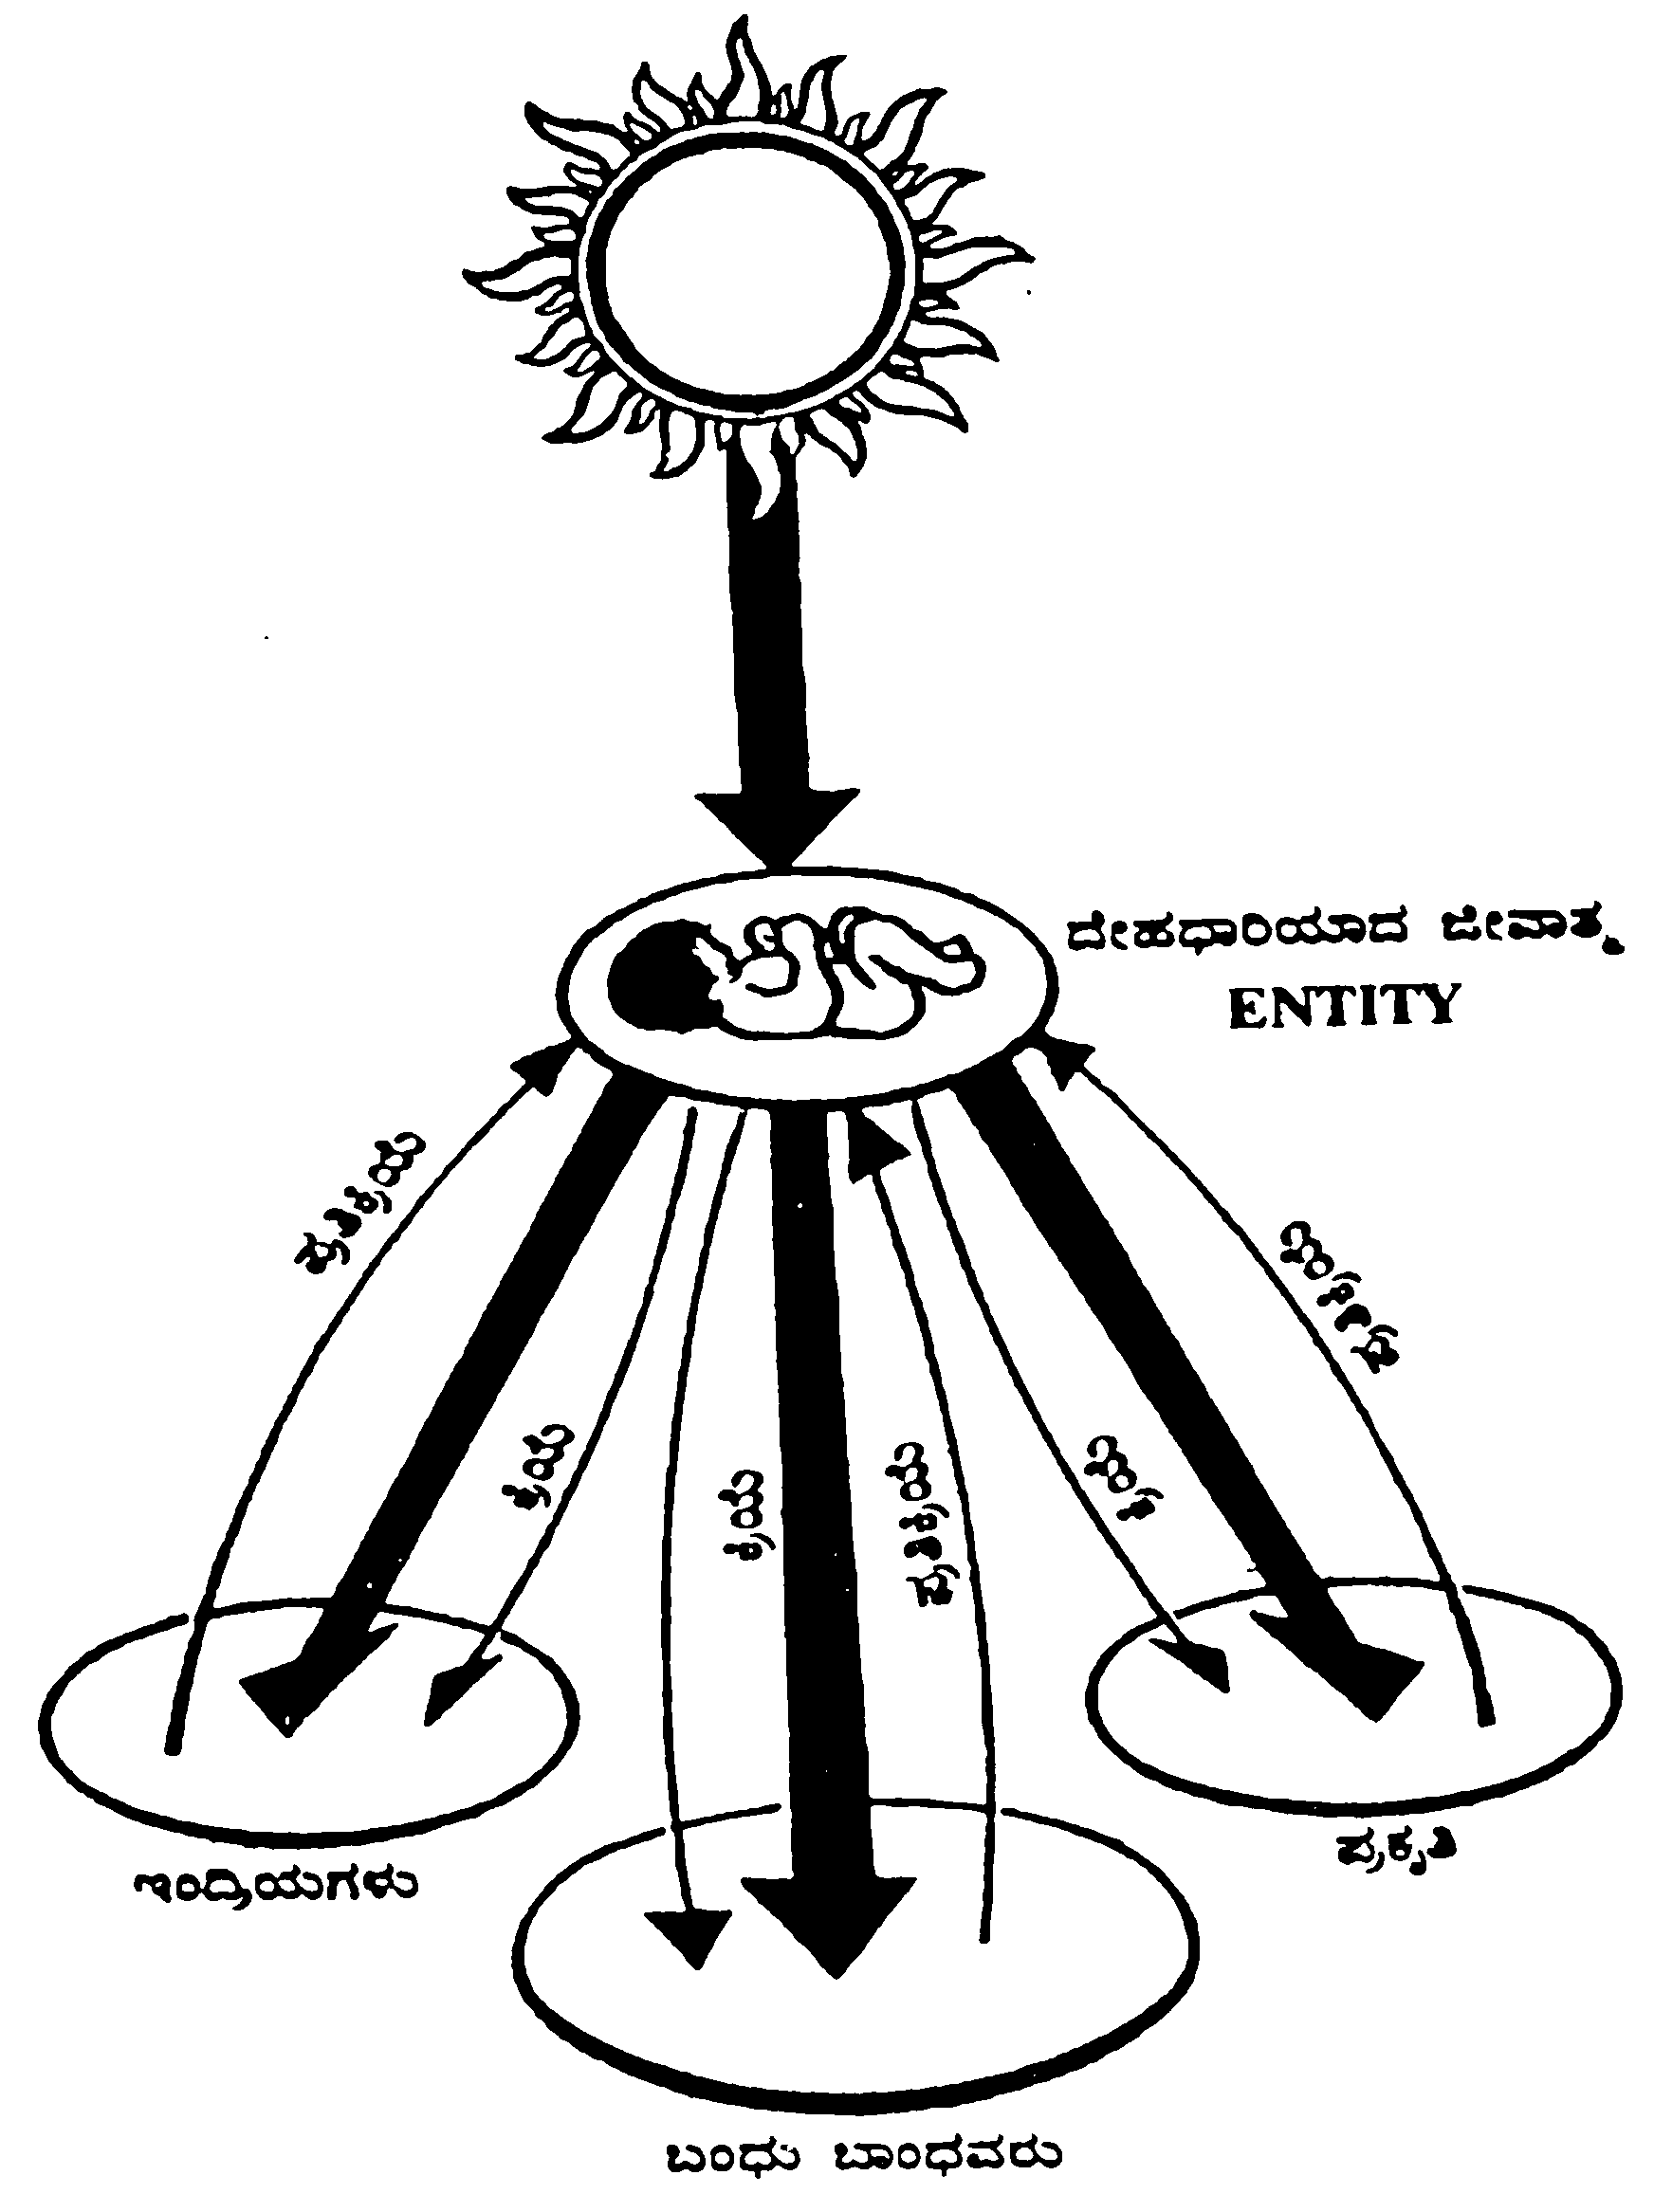
\includegraphics[scale=0.8]{"images/chap6_fig1.png"}
\end{center}

ಇಲ್ಲಿರುವ ಅಮರನಾದ ಜೀವಾತ್ಮನನ್ನು ಕೇಸೀ \enginline{Immortal Entity (}ಇಮ್ಮಾರ್ಟಲ್ ಎಂಟಿಟಿ) ಎಂದು ಕರೆದರೆ, ದೇಹಧಾರಿಯಾದ ಜೀವಾತ್ಮನನ್ನು \enginline{Entity (}ಎಂಟಿಟಿ) ಎಂದು ಕರೆಯುತ್ತಾನೆ. ಇಲ್ಲಿ ಅದನ್ನೇ ಜೀವಿ ಅಥವಾ ಜೀವಾತ್ಮನೆಂದು ಕರೆದಿದೆ. ಚಿತ್ರದಲ್ಲಿ ತೋರಿಸಿದಂತೆ, ಅಮರವಾದ ಜೀವಾತ್ಮ ದೇಹಧಾರಿಯಾದಾಗ, ಆ ಜೀವಿಯ ವ್ಯಕ್ತಿತ್ವ ಮೂರು ಕ್ಷೇತ್ರಗಳ ವ್ಯವಹಾರಗಳಿಂದ ಪುಟಗೊಳ್ಳುತ್ತದೆ. ಇಲ್ಲಿ ಕಾಣುವಂತೆ ಅವೇ ಆ ಜೀವಿಯ ವ್ಯಕ್ತಿತ್ವದ ಆಧಾರಸ್ತಂಭಗಳೆಂದರೂ ತಪ್ಪಾಗದು. ಅವುಗಳಲ್ಲಿ ಮೊದಲನೆಯದು ವ್ಯಕ್ತಿಯ ಶರೀರ ಇಂದ್ರಿಯಗಳು, ಎರಡನೆಯದು ಸುತ್ತುಮುತ್ತಲಿನ ಪ್ರಕೃತಿ ಮತ್ತು ಕೊನೆಯದು, ಬಂಧುಬಾಂಧವರಿರುವ ಸಮಾಜ. ಈ ಮೂರು ಕ್ಷೇತ್ರಗಳಲ್ಲಿಯೂ ಆ ಜೀವಿ ತೋರುವ ಕ್ರಿಯೆಗಳಿಗೆಲ್ಲ ತಕ್ಕ ಪ್ರತಿಕ್ರಿಯೆಗಳು ಆ ಜೀವಿಯ ಆಂತರ್ಯದಲ್ಲಿ ದಾಖಲಾಗುತ್ತಲಿರುತ್ತವೆ.

ಹೀಗೆ, ಹೊಟ್ಟೆಬಾಕತನವೆಂಬ ಕ್ರಿಯೆಗೆ, ಈ ಜನ್ಮದಲ್ಲಾಗಲೀ, ಮುಂದಿನ ಜನ್ಮದಲ್ಲಾಗಲೀ ಜೀರ್ಣಾಂಗವ್ಯೂಹವೇ ಕೆಟ್ಟು, ಅಜೀರ್ಣ ವ್ಯಾಧಿಯ ಪ್ರತಿಕ್ರಿಯೆ ವ್ಯಕ್ತವಾಗುತ್ತದೆ. ಹಾಗಲ್ಲದೆ, ಪ್ರಕೃತಿಯ ಶಕ್ತಿಗಳನ್ನಾತ ಊರ್ಜಿತಗೊಳಿಸಿದರೆ, ಪ್ರಕೃತಿಯ ಪ್ರತಿಕ್ರಿಯೆ ಅವನ ಉನ್ನತಿಗೆ ಸಾಧಕವಾಗುತ್ತದೆ. ಬದಲಿಗೆ, ಪ್ರಕೃತಿಗೇ ಕೇಡು ಬಗೆದರೆ, ಅವನಿಗೆ ಕೇಡುಗಾಲ ತಪ್ಪಿದ್ದಲ್ಲ. ಇನ್ನು ಸಮಾಜದ ಬಂಧು ಬಾಂಧವರೊಳಗಿನ ಕ್ರೂರ ವರ್ತನೆ, ಆ ವ್ಯಕ್ತಿಗೆ ತಿರುಗುಬಾಣವಾಗಿ ಹಿಂಸೆ\break ಕೊಡಬಹುದು. ಕೇಸೀಯ ದಾಖಲೆಗಳಲ್ಲಿ ಈ ಎಲ್ಲ ರೀತಿಗಳ ಬೇಕಷ್ಟು ಉದಾಹರಣೆಗಳು\break ದೊರಕುತ್ತವೆ.

ಟೆನ್ನಿಸ್ ಆಟದ ಒಂದು ಸಾಮಾನ್ಯ ಉದಾಹರಣೆಯನ್ನು ಹೇಳಿದರೆ ವಿಭಿನ್ನ ದೇಹಗಳಲ್ಲಿ ರಂಗಗಳಲ್ಲಿ ವ್ಯಕ್ತಿಯು ಅನುಭವಿಸುವ ಕರ್ಮಫಲವನ್ನು ಅರ್ಥಮಾಡಿಕೊಳ್ಳಬಹುದು. ಒಂದು ಕ್ರೀಡಾಂಗಣದಲ್ಲಿ ಇಬ್ಬರು ಟೆನ್ನಿಸ್ ಆಡುತ್ತಿದ್ದಾರೆಂದೆಣಿಸಿ. ಅವರಿಬ್ಬರೂ ೫–೫ ಅಂಕಗಳಿಸಿ ಆಡುತ್ತಿರುವಾಗಲೇ ನಿಗದಿತ ಸಮಯವು ಮುಗಿದರೆ, ಅವರು ಆಟವನ್ನೇನೋ ನಿಲ್ಲಿಸಿ ಕ್ರೀಡಾಂಗಣದಿಂದ ಹೊರನಡೆಯುತ್ತಾರೆ. ಆದರೆ ಆ ಆಟದ ಗೀಳು ಅವರನ್ನು ಬಿಡುವುದಿಲ್ಲ. ಹಾಗಾಗಿ, ಬೇಕಿದ್ದರೆ ಸ್ವಲ್ಪ ವಿಶ್ರಾಂತಿಯ ಬಳಿಕ, ಬೇರೊಂದು ಕ್ರೀಡಾಂಗಣಕ್ಕೆ ತೆರಳಿಯಾದರೂ ಆ\break ಆಟವನ್ನು ಮುಂದುವರಿಸಲು ಅವರು ನಿರ್ಧರಿಸುತ್ತಾರೆ. ಕ್ರೀಡಾಂಗಣ ಬದಲಾದರೂ ಅವರ ಆಟ ಹಿಂದೆ ಗಳಿಸಿದ ಅಂಕಗಳ ಆಧಾರದಿಂದಲೇ ಮುಂದುವರಿಯುತ್ತದೆ. ಅವರೀಗ ಬೇರೆ ಕ್ರೀಡಾಂಗಣದಲ್ಲಿ ಆಡುತ್ತಿರುವುದು ಎಷ್ಟು ನಿಚ್ಚಳವೋ, ಅಷ್ಟೇ ನಿಚ್ಚಳ ಅವರು ಹಿಂದಿನ ಆಟದಲ್ಲಿ ಗಳಿಸಿದ ಅಂಕಗಳನ್ನೇ ಮುಂದುವರಿಸಿಕೊಂಡು ಹೋಗುತ್ತಿದ್ದಾರೆಂಬುದು. ಹಾಗೆಯೇ ಈ ಜಗತ್ತಿಗೆ ಬಂದ ಆತ್ಮವೊಂದು ದೇಹದಿಂದ ದೇಹಕ್ಕೆ ತೆರಳುತ್ತಾ ಸಂಚಿತ ಸಂಸ್ಕಾರದ ಅಂಕಗಳಿಗೇನೇ ಮತ್ತಷ್ಟನ್ನು ಸೇರಿಸುತ್ತಾ ಜೀವನ ಹೋರಾಟ ನಡೆಸುತ್ತಿರುತ್ತದೆ.


\section*{ಕರ್ಮದ ಪ್ರತೀಕಾರಗಳು}

\addsectiontoTOC{ಕರ್ಮದ ಪ್ರತೀಕಾರಗಳು}

‘ಮನುಷ್ಯನ ಶರೀರದಲ್ಲಿರುವ ಗ್ರಂಥಿಗಳ ಸ್ವರೂಪ ಮತ್ತು ಚಟುವಟಿಕೆಗಳು ಜೀವಿಯ ಪೂರ್ವಕರ್ಮಗಳನ್ನು ಸೂಕ್ಷ್ಮವಾಗಿ ತಿಳಿಸುವ ಆತ್ಯುತ್ತಮ ಸಾಧನಗಳು’\footnote{\engfoot{Glands themselves are focal points for the expression of the heredity of the psyche for its Karma.}} ಎಂದು ಕೇಸೀ ಹೇಳುತ್ತಾನೆ. ಅವನು ಕೊಡುವ ಕೆಲವು ನಿದರ್ಶನಗಳಿವು–

೧.\ ಕೊಬ್ಬಿನಿಂದಾಗಿ ವಿಪರೀತ ದಪ್ಪವಾಗಿ ಬೆಳೆದಿದ್ದ ಸುಂದರಿಯೊಬ್ಬಳು ದುಃಖಿತಳಾಗಿ ಕೇಸೀಯ ಬಳಿ ತನ್ನ ದುರವಸ್ಥೆಯ ಬಗೆಗೆ ಕೇಳಿದಾಗ ‘ಎರಡು ಜನ್ಮಗಳ ಹಿಂದೆ ರೋಮಿನಲ್ಲಿ ಪ್ರಸಿದ್ಧ ಕ್ರೀಡಾಪಟುವಾಗಿದ್ದ ನೀನು ದೇಹಭಾರದಿಂದ ನಿನ್ನಷ್ಟು ಚುರುಕಾಗಿ ಓಡಾಡದಿದ್ದವರನ್ನು ಅತ್ಯಂತ ಹೀನಾಯವಾಗಿ ವಿಪರೀತ ಹಾಸ್ಯ ಮತ್ತು ನಿಂದೆ ಮಾಡಿ ನೋಯಿಸಿದ್ದಿ. ಈ ಜನ್ಮದಲ್ಲಿ ಅಂತಹ ಕೆಲಸಕ್ಕೆ ಅವಕಾಶವೇ ಇಲ್ಲದಂತೆ ಈ ಅವಸ್ಥೆ’ ಎಂದು ತಿಳಿಸಿದ.

೨.\ ತನ್ನ ಹಿಂದಿನ ಜನ್ಮದಲ್ಲಿ ಫ್ರೆಂಚ್ ಕಾನ್ವೆಂಟಿನಲ್ಲಿ ಅಧ್ಯಾಪಕಿಯಾಗಿದ್ದು, ತಪ್ಪು ಮಾಡುವುದು ಮಕ್ಕಳ ಸಹಜ ಸ್ವಭಾವ, ತಾಳ್ಮೆಯಿಂದ ಅದನ್ನು ತಿದ್ದುವುದು ಅಧ್ಯಾಪಕಿಯಾದ ತನ್ನ ಕರ್ತವ್ಯ ಎಂಬುದನ್ನು ತಿಳಿಯದೆ,ಅಲ್ಲಿನ ಚಿಕ್ಕಚಿಕ್ಕ ವಿದ್ಯಾರ್ಥಿಗಳಿಗೆ ಅತಿ ಕಠಿಣವಾದ ಶಿಕ್ಷೆಯನ್ನು ನಿಷ್ಕರುಣೆಯಿಂದ ಕೊಟ್ಟ ಒಬ್ಬಾಕೆಯ ದಾರುಣ ಕತೆ ಕೇಸೀಯ ದಾಖಲೆಗಳಲ್ಲಿದೆ. ಈಗಿನ ಜನ್ಮದಲ್ಲಿ\break ಗ್ರಂಥಿ\-ಗಳ ಅತಿ ಚಟುವಟಿಕೆಯಿಂದ ವಿಪರೀತ ರಕ್ತಸ್ರಾವದಿಂದ ನರಳುವಂತಾಗಿ, ತಿಂಗಳಿಗೆ ಹದಿ\-ನೈದು ದಿನಗಳ ಕಾಲ ಆಕೆ ಹಾಸಿಗೆಯಲ್ಲೇ ಇರಬೇಕಾದಂತಹ ಪರಿಸ್ಥಿತಿಯುಂಟಾಗಿ, ತನ್ನ\break ವಿದ್ಯಾಭ್ಯಾಸವನ್ನು ಮುಂದುವರಿಸಲು ಅಸಮರ್ಥಳಾದಳು. ಜೀವನದುದ್ದಕ್ಕೂ ಅವಳ ಪಾಲಿಗೆ ಸಂಕಟವೇ ಒದಗಿತು. ಮದುವೆಯಾಗಲು ತವಕಿಸಿ ಕೊನೆಗೆ ಹೇಗೋ ಅತ್ಯಂತ ಕಷ್ಟದಿಂದ ಮದುವೆಯಾದರೂ ಕೆಲವೇ ದಿನಗಳಲ್ಲಿ ವಿಚ್ಛೇದವೂ ಆಯಿತು. ಕುಡಿತದ ಅಭ್ಯಾಸಕ್ಕೆ ಸಿಲುಕಿ ನರಳಿ ನರಳಿ, ಆತ್ಮಹತ್ಯೆಯನ್ನು ಮಾಡಿಕೊಂಡು ಆಕೆ ಒಂದು ದಿನ ಕಣ್ಮರೆಯಾದಳು.

೩.\ ಇಪ್ಪತ್ತೊಂದು ವರ್ಷ ವಯಸ್ಸಿನ ವ್ಯಗ್ರ ಯುವಕನಾತ. ಕೆಥೋಲಿಕ್ ಸಂಪ್ರದಾಯಕ್ಕೆ ಸೇರಿದ ಆತನ ಗುರುಹಿರಿಯರು, ಅವನನ್ನು ಪಾದ್ರಿಯಾಗುವಂತೆ ಪ್ರೇರಿಸಿದ್ದರು. ಆದರೆ ಅವನೇನೂ ಆ ಜೀವನದ ಕುರಿತಾಗಿ ಆಕರ್ಷಿತನಾಗಲಿಲ್ಲ. ಸಲಿಂಗರತಿಯ ಬಗೆಗಿನ ತೀವ್ರ ಹಂಬಲ ಅವನನ್ನು ಬಹಳವಾಗಿ ಕಾಡಿತು. ಆತನೇ ಕೇಸೀಯ ಬಳಿ ಹೋದಾಗ ‘ಹಿಂದಿನ ಜೀವನದಲ್ಲಿ ಫ್ರೆಂಚ್ ಆಸ್ಥಾನದಲ್ಲಿದ್ದ ನೀನು ಹಲವು ಆಸ್ಥಾನಿಕರ ಸಲಿಂಗರತಿಯ ಕಳಂಕಮಯ ಜೀವನವನ್ನು ಬಯಲಿಗೆಳೆದಿದ್ದೆ. ಇತರರ ದೌರ್ಬಲ್ಯಗಳನ್ನು ಅತ್ಯಂತ ನಿಂದನೀಯವಾಗಿ ಟೀಕಿಸುವುದು ನಿನಗೆ ತುಂಬ ಸಂತೋಷದ ಕೆಲಸವಾಗಿತ್ತು. ನಿನ್ನ ವ್ಯಂಗ್ಯಚಿತ್ರ ರಚನಾಸಾಮರ್ಥ್ಯವನ್ನು ಇದಕ್ಕಾಗಿಯೇ ಉಪಯೋಗಿಸಿದ್ದಿ’ ಎಂದು ತಿಳಿಸಿ, ಕೊನೆಯಲ್ಲಿ ‘ಬೇರೆಯವರು ನಿನ್ನನ್ನು ಹೀನಾಯ ಮಾಡಬಾರ ದೆಂದಿದ್ದರೆ ನೀನು ಇತರರನ್ನು ಹೀನಾಯ ಮಾಡಬೇಡ. ನೀನು ಯಾವ ಮಟ್ಟದಲ್ಲಿ ಇತರರನ್ನು ಹೀನೈಸಿದ್ದೆಯೋ, ಅದೇ ಮಟ್ಟದಲ್ಲಿ ನೀನೂ ನಿಂದಿಸಲ್ಪಡುವೆ ಬೇರೆಯವರಿಂದ. ಯಾವುದನ್ನು ಕಂಡು ನಿಂದಿಸಿ ಅಸಹ್ಯಪಡುವೆಯೋ ಅದೇ ನಿನ್ನಲ್ಲಿ ಮೂಡುವುದು\footnote{\engfoot{What you condemn in others that you become in yourself.}} ಎಂದನು.

ಇನ್ನೊಬ್ಬರ ದುಃಖಸಂಕಟಗಳನ್ನು ತಿಳಿದುಕೊಳ್ಳದೆ, ಸಹಾನುಭೂತಿ ತೋರದೆ, ತನ್ನ ಜ್ಞಾನ ಸಂಸ್ಕೃತಿಯ ಅಭಿಮಾನದ ಶ್ರೇಷ್ಠತೆಯನ್ನು ತೋರ್ಪಡಿಸುವ ದುರಹಂಕಾರದ ವರ್ತನೆಯು, ತೀವ್ರ ಕರ್ಮದ ಆಘಾತಗಳನ್ನು ಉಂಟುಮಾಡುತ್ತದೆಂದು ಕೇಸೀ ಮತ್ತೆ ಮತ್ತೆ ಹೇಳುತ್ತಾನೆ. ಅದಕ್ಕೆ ಒಂದು ಉದಾಹರಣೆ ಇಲ್ಲಿದೆ–

೪. ಸೈನ್ಯದಲ್ಲಿ ಲೆಫ್ಟಿನೆಂಟಾಗಿ ಕೆಲಸ ಮಾಡುತ್ತಿದ್ದ ಇಪ್ಪತ್ತೇಳು ವರ್ಷ ವಯಸ್ಸಿನ ಯುವಕನೊಬ್ಬ ಆತ್ಮವಿಶ್ವಾಸಹೀನನಾಗಿ ಕೀಳರಿಮೆಯಿಂದ ಅವಸಾದವನ್ನು ಹೊಂದಿದ್ದ. ತನ್ನ ಸಾಮರ್ಥ್ಯದಲ್ಲೇ ಆತನಿಗೆ ವಿಪರೀತ ಸಂಶಯ. ಈ ಹೀನ ಪರಿಸ್ಥಿತಿಗೆ ಕಾರಣವನ್ನು ಕಂಡುಹಿಡಿಯಲಾಗದೆ, ಆತ ಕೇಸೀಯ ಬಳಿಗೆ ಹೋದ. ಆಗ ‘ಈತ ತನ್ನ ಹಿಂದಿನ ಜೀವನದಲ್ಲಿ ಒಬ್ಬ ಸಾಹಿತ್ಯ ವಿಮರ್ಶಕನಾಗಿದ್ದ. ತನ್ನ ಅಭಿರುಚಿಗೆ ಸೇರದ ವಿಷಯಗಳನ್ನು ನಿರ್ದಯವಾಗಿ ಅತ್ಯಂತ ಕಟುನುಡಿಗಳಿಂದ ನಿಂದಿಸಿ, ಟೀಕಿಸುತ್ತಿದ್ದ. ಅಸಂಖ್ಯ ಜನರ ಹೃದಯದಲ್ಲಿ ಸಂಶಯ, ಗೊಂದಲವನ್ನು ತಂದ ಈತ, ತಾನೇ ಸಂಶಯ, ಗೊಂದಲಗಳಿಂದ ಈಗ ನರಳುತ್ತಿದ್ದಾನೆ\footnote{\engfoot{As you criticized, know that you yourself must be criticized.}} ಎಂಬುದು ಕೇಸೀಯ ಮತ.

ಜಗತ್ತಿನಲ್ಲಿ ನಿಜವಾದ ವಿಮರ್ಶಕನ ಉದ್ಯೋಗವನ್ನು ಮಾಡುವವರ ಸಂಖ್ಯೆ ಅತಿವಿರಳ. ಉಳಿದವರು ಅಭಿಪ್ರಾಯ ಸ್ವಾತಂತ್ರ್ಯದ ಹೆಸರಿನಲ್ಲಿ, ವಿಮರ್ಶೆಯ ನೆಪದಲ್ಲಿ, ತಮ್ಮ ಅಹಂ ಕಾರ, ಮಮಕಾರಗಳನ್ನು ಪ್ರದರ್ಶಿಸುತ್ತ, ಇತರರನ್ನು ನಿಂದಿಸುವ ಕೆಲಸ ಮಾಡುತ್ತಿರುತ್ತಾರೆ. ಲಂಗುಲಗಾಮಿಲ್ಲದೆ ತಮ್ಮ ನಾಲಗೆಯನ್ನು ಹರಿಯಬಿಡುತ್ತಾರೆ. ಇತರರ ರೀತಿನೀತಿ, ನಡೆನುಡಿ, ಸುಖದುಃಖಗಳನ್ನು ತನಗೆ ಸರಿಯಾಗಿ ಅರಿಯುವ ಸಾಮರ್ಥ್ಯವಿಲ್ಲದಿದ್ದರೂ, ಯಾರು ಅಸಂಬದ್ಧ ಪ್ರಲಾಪ ಮಾಡುತ್ತಾ ಟೀಕೆ ಮಾಡುವರೋ, ಇತರರನ್ನು ಹಳಿಯುವರೋ, ಅಂಥವರು ತಮ್ಮ ‘ಅಹಂ’ನ್ನು ಒಂದೇಸಮನೆ ಹೆಚ್ಚಿಸಿಕೊಂಡು, ತಾವು ಪರರಿಗಿಂತ ಶ್ರೇಷ್ಠರೆಂದು ತಿಳಿದು ಇತರರಿಗೆ ನಿಂದನೆಯ ಸುರಿಮಳೆಯನ್ನು ಹರಿಯಿಸುವರು. ಅದರಿಂದ ಕೊಬ್ಬಿದ ‘ಅಹಂ’ ಮತ್ತೊಂದು ಜನ್ಮದಲ್ಲಿ ನಿಕೃಷ್ಟಮಟ್ಟದಲ್ಲಿಯೇ ಇರಬೇಕಾದ ಪರಿಸ್ಥಿತಿ ಬರುತ್ತದೆ. ರಚನಾತ್ಮಕ ಟೀಕೆ ಮಾಡ ಬಾರದು ಎಂದು ಇದರರ್ಥ ಅಲ್ಲ. ಇತರರ ದೋಷವನ್ನು ಭೂತಕನ್ನಡಿಯಿಂದ ನೋಡಿ ಚಪ್ಪರಿಸುತ್ತ ನಿಂದಿಸುವ ಚಟ ದುರಹಂಕಾರದ ದುಷ್ಟತನ. ಅದರ ಫಲವನ್ನು ಉಣ್ಣಲೇ ಬೇಕಾಗುವುದು ಎಂಬುದು ಕೇಸೀಯ ಅಭಿಪ್ರಾಯ ಮತ್ತು ಇಲ್ಲಿ ಗಮನಿಸಬೇಕಾದ ಅಂಶ.


\section*{ದುಷ್ಕರ್ಮಗಳ ವೈವಿಧ್ಯ}

\addsectiontoTOC{ದುಷ್ಕರ್ಮಗಳ\break ವೈವಿಧ್ಯ}

ಪರರ ನರಳಾಟವನ್ನು ಕಂಡೂ ಕಾಣದಂತೆ ನಟಿಸುವುದು ದೋಷ ಅಥವಾ ಅಪರಾಧವಾಗುತ್ತದೆ ಎನ್ನುತ್ತಾನೆ ಕೇಸೀ. ಸಹಾನುಭೂತಿಯನ್ನು ತೋರಿಸಬೇಕಾದಲ್ಲಿ ಅದನ್ನು ತೋರಿಸದಿದ್ದರೆ, ಆಗ ಮಾಡಬೇಕಾದ ಕಾರ್ಯವನ್ನು ಮಾಡದ ತಪ್ಪಿಗೆ \enginline{(Sin of Omission)} ಭಾಗಿಗಳಾಗುತ್ತೇವೆ. ಆರ್ತರಿಗೆ, ಕಷ್ಟದಲ್ಲಿ ಸಿಲುಕಿದವರಿಗೆ ಸಹಾಯ ಮಾಡುವುದಿರಲಿ, ಅವರ ಮನನೋಯುವಂತೆ ಟೀಕಿಸಿ, ಹೀಯಾಳಿಸುವುದರಿಂದಲೂ ಮಾಡಬಾರದ ಕೆಲಸ ಮಾಡಿದ ತಪ್ಪಿಗೆ \enginline{(Sin of Commission)} ಒಳಗಾಗುತ್ತೇವೆ. ಅಂತಹ ದುಷ್ಕರ್ಮದ ಫಲ ಏನು ಗೊತ್ತೆ?


\section*{ನಿದರ್ಶನಗಳ ಸಾಕ್ಷ್ಯ}

\addsectiontoTOC{ನಿದರ್ಶನಗಳ ಸಾಕ್ಷ್ಯ}

೧.\ ಈ ಜನ್ಮದಲ್ಲಿ ಹುಟ್ಟುಕಿವುಡಾಗಿರುವ ವ್ಯಕ್ತಿ, ಪೂರ್ವಜನ್ಮದಲ್ಲಿ ಸಹಾಯಕ್ಕಾಗಿ ಅಂಗಲಾಚಿ ದೈನ್ಯದಿಂದ ಬೇಡುವವರಿಗೆ ಕಿವುಡನಂತೆಯೇ ವರ್ತಿಸಿದ್ದ.

೨.\ ಈ ಜೀವನದಲ್ಲಿ ಬೆನ್ನುಮೂಳೆಯ ಕ್ಷಯದಿಂದ ನರಳುವ ವ್ಯಕ್ತಿಯೊಬ್ಬ, ತನ್ನ ಹಿಂದಿನ ಜೀವನದಲ್ಲಿ ಇತರರನ್ನು ಮೊನಚಾದ ಮಾತುಗಳಿಂದ ಇರಿದು ತೀವ್ರವಾಗಿ ನೋಯಿಸಿದವನಾಗಿದ್ದ.

೩.\ ತೀವ್ರವಾದ ಅಸ್ತಮಾರೋಗದಿಂದ ನರಳುವಾತ, ತನ್ನ ಹಿಂದಿನ ಜೀವನದಲ್ಲಿ ಇನ್ನೊಬ್ಬರ ಬಾಳನ್ನು ಮೆಟ್ಟಿಯೇ ಬದುಕಿದವನಾಗಿದ್ದ. ತನ್ನ ಬಾಳಿಗೂ ಒಂದಾನೊಂದು ದಿನ ಕಷ್ಟ ಬಂದೀತೆಂಬ ಕಲ್ಪನೆ ಎಂದೂ ಆ ಜನ್ಮದಲ್ಲಿ ಆತನನ್ನು ಕಾಡಿರಲಿಲ್ಲ. ಈ ಜನ್ಮದಲ್ಲಿ ಅದರ ಫಲ ಆತ ಉಣ್ಣಬೇಕಾಗಿದೆ.

೪.\ ಹನ್ನೊಂದು ವರ್ಷ ವಯಸ್ಸಾದರೂ ಹುಡುಗನೊಬ್ಬ ಹಾಸಿಗೆಯಲ್ಲಿ ರಾತ್ರಿ ಹೊತ್ತು ಮೂತ್ರ ಮಾಡಿಕೊಳ್ಳುತ್ತಿದ್ದ. ಆತನ ತಂದೆತಾಯಿಗಳು ಆ ದುರಭ್ಯಾಸವನ್ನು ಹೋಗಲಾಡಿಸಲು ಬಹಳ ಶ್ರಮಪಟ್ಟರೂ ಸಫಲರಾಗಲಿಲ್ಲ. ಕೊನೆಗೆ ಕೇಸೀಯನ್ನು ಕೇಳಿಕೊಂಡಾಗ ಆ ಹುಡುಗನ ಸಮಗ್ರ ಕರ್ಮದ ಹಿನ್ನೆಲೆಯ ಅರಿವಾಯಿತು–

ಪ್ಯೂರಿಟನ್ನರ ಕಾಲದಲ್ಲಿ ಫ್ರಾನ್ಸಿನ ಆಸ್ಥಾನದಲ್ಲಿದ್ದ ಆತ ಮಂತ್ರಿಯಾಗಿದ್ದ. ಶಿಕ್ಷೆಗೆ ಗುರಿ\-ಯಾದ\-ವರನ್ನು ಕೊಳವೊಂದಕ್ಕೆ ನೂಕಿ ಅವರ ಕಷ್ಟವನ್ನೂ, ನರಳಾಟವನ್ನೂ ಕಂಡು ಆನಂದಪಡುತ್ತಿದ್ದ. ಆ ದುಷ್ಟಕ್ರಿಯೆಯ ಸಂಕೇತವೋ ಎಂಬಂತೆ, ಈ ಜನ್ಮದಲ್ಲಿ ರಾತ್ರಿ ಹೊತ್ತು ಮೂತ್ರದ ಹೊಳೆಯಲ್ಲಿ ತಾನೇ ಬಿದ್ದುಕೊಳ್ಳುವ ಪರಿಸ್ಥಿತಿ ಅವನಿಗೆ ಬಂದಿತ್ತು. ಕೇಸೀಯ ಸಲಹೆಯನ್ನು ತಂದೆತಾಯಿಗಳು ಅನುಸರಿಸಿದಾಗ ಹುಡುಗನಲ್ಲಿ ಬದಲಾವಣೆ ಕಂಡುಬಂತು. ರಾತ್ರಿ ನಿದ್ರಿಸಲು ಆರಂಭಿಸಿದಾಗ ಹುಡುಗನ ಕಿವಿಯಲ್ಲಿ ‘ನೀನು ಒಳ್ಳೆಯವನು, ನೀನು ಎಂದಿಗೂ ಇಂತಹ ಅಸಹ್ಯ ತಪ್ಪುಗಳನ್ನು ಮಾಡಲಾರೆ. ನಿನ್ನಿಂದ ಒಳಿತನ್ನೇ ನಿನ್ನ ಹಿರಿಯರು ನಿರೀಕ್ಷಿಸುತ್ತಿದ್ದಾರೆ. ಅಜ್ಞಾನದಿಂದುಂಟಾದ ದುಷ್ಕರ್ಮಕ್ಕಾಗಿ ನೀನು ನಿಜವಾಗಿಯೂ ಪಶ್ಚಾತ್ತಾಪ ಪಟ್ಟಿದ್ದಿ’ ಎಂದು ಒಂದು ವಾರದವರೆಗೆ ಹೇಳಿದರು. ನಂತರ ವಾರಕ್ಕೊಮ್ಮೆ, ಬಳಿಕ ತಿಂಗಳಿಗೊಮ್ಮೆ, ಆ ಮಾತುಗಳನ್ನು ಹೇಳುತ್ತಿದ್ದರು. ಹುಡುಗನು ಸ್ವಲ್ಪಕಾಲದಲ್ಲೇ ಆ ದುರಭ್ಯಾಸದಿಂದ ಪಾರಾದ.


\section*{ಬೇಡ ನಿರಾಶಾವಾದ}

\addsectiontoTOC{ಬೇಡ ನಿರಾಶಾವಾದ}

ಕರ್ಮವೆಂದರೆ ದುಷ್ಕರ್ಮಫಲವೆಂದೇ ಅರ್ಥವಲ್ಲ. ಯಾವ ಕರ್ಮವೂ ವ್ಯರ್ಥವಾಗದು – ಅದರ ಫಲ ದೊರೆತೇ ದೊರೆಯುತ್ತದೆ ಎನ್ನುತ್ತಾನೆ ಕೇಸೀ. ನಿಷ್ಪಕ್ಷಪಾತವಾಗಿ ಕರ್ಮನಿಯಮ ಕೆಲಸ ಮಾಡುವುದರಿಂದ, ನಮ್ಮ ದುಷ್ಕರ್ಮಗಳಿಗೆ ಸರಿಯಾದ ಶಿಕ್ಷೆ ದೊರಕುವುದಲ್ಲದೇ, ಸತ್ಕರ್ಮಗಳಿಗೆ ಯೋಗ್ಯವಾದ ಬಹುಮಾನವೂ ದೊರಕುವುದು. ಈ ನಿಯಮವನ್ನು ಸರಿಯಾಗಿ ಸ್ಪಷ್ಟವಾಗಿ ತಿಳಿದುಕೊಂಡಲ್ಲಿ ನಿರಾಶಾವಾದ ನಮ್ಮ ಬಳಿ ಸುಳಿಯದು. ನಮ್ಮ ಕೃತ್ಯಗಳಿಂದ ಪ್ರತಿಕ್ಷಣವೂ ನಾವು ನಮ್ಮ ಭವಿಷ್ಯವನ್ನು ನಿರ್ಮಿಸುತ್ತಿದ್ದೇವೆ\footnote{\engfoot{At every instant, we are creating our own future and dictating the terms of future.}} ಎಂಬುದನ್ನು ಅರಿತು ಸುಧಾ ರಣೆಯ ದಾರಿ ತುಳಿಯಬೇಕೆನ್ನುವ ಕೇಸೀ ಉಲ್ಲೇಖಿಸಿದ ಒಂದು ಘಟನೆ ಹೀಗಿದೆ:

ಅಮೇರಿಕದಲ್ಲಿ, ತರುಣಿಯೋರ್ವಳ ಅತಿ ಸುಂದರ ಹಸ್ತಗಳ ಛಾಯಾಚಿತ್ರಕ್ಕೆ ಉಗುರು ಶೃಂಗಾರ ಸಾಧನಗಳ ಪ್ರಚಾರಕ್ಕಾಗಿ, ಹೆಚ್ಚಿನ ಕಂಪೆನಿಗಳಿಂದ ವಿಶೇಷ ಬೇಡಿಕೆಗಳು ಬರುತ್ತಿದ್ದವು. ಕಂಪೆನಿಯ ಏಜಂಟರುಗಳು ಆಕೆಯ ಹಸ್ತಗಳ ಛಾಯಾಚಿತ್ರಕ್ಕಾಗಿ ಬಹಳಷ್ಟು ಸ್ಪರ್ಧೆಯಿಂದ ಮುನ್ನುಗ್ಗುತ್ತಿದ್ದರು. ಆಕೆ ಕೇಸೀಯಲ್ಲಿ ತನ್ನ ಬಗೆಗೆ ‘ಹೇಳಿಕೆ’ಯನ್ನು ನೀಡಬೇಕೆಂದು ಕೇಳಿಕೊಂಡಳು. ಆಗ ತಿಳಿದುದಿಷ್ಟು–‘ಅವಳು ತನ್ನ ಹಿಂದಿನ ಜೀವನದಲ್ಲಿ ಇಂಗ್ಲೆಂಡ್​ನ ಕಾನ್ವೆಂಟೊಂದ\-ರಲ್ಲಿ ತನ್ನ ಜೀವನವನ್ನೆಲ್ಲಾ ಅನಾಥ ಮಕ್ಕಳ ಶುಶ್ರೂಷೆಯಲ್ಲಿ ಕಳೆದಿದ್ದಳು. ಇತರರ ದೃಷ್ಟಿಯಲ್ಲಿ ಅಸಹ್ಯ\-ವೆನಿಸ\-ಬಹುದಾದ ಕೆಲಸವನ್ನು ‘ಹೇ ಭಗವಾನ್, ನನ್ನನ್ನು ಈ ಸ್ಥಾನದಲ್ಲಿರಿಸಿ ದ್ದೀಯೆ. ನಾನು ಈ ಎಲ್ಲಾ ಕೆಲಸಗಳನ್ನೂ ಮಾಡುತ್ತೇನೆ. ನಿನ್ನ ಪ್ರೀತಿಗಾಗಿ ಮಾಡುತ್ತೇನೆ. ಅದನ್ನು ಸರಿಯಾಗಿ ಶ್ರದ್ಧೆಯಿಂದ ಮಾಡುವ ಶಕ್ತಿಯನ್ನು ಕೊಡು’ ಎಂದು ದಿನವೂ ಪ್ರಾರ್ಥಿಸುತ್ತ, ಪೂರ್ಣ ಸಮರ್ಪಣೆಯ ಜೀವನ ನಡೆಯಿಸಿದ್ದಳು. ‘ಪುಟ್ಟ ಮಕ್ಕಳ ದೇಹ, ಮನಸ್ಸು ಆತ್ಮ– ಇವುಗಳ ಉನ್ನತಿಗಾಗಿ ತನ್ನನ್ನೇ ಸಮರ್ಪಿಸಿಕೊಂಡು ಶ್ರದ್ಧೆಯಿಂದ ದುಡಿದದ್ದಕ್ಕಾಗಿ ಈ ಜೀವಿಯ ದೇಹ, ಮನಸ್ಸು, ಆತ್ಮಗಳು ಇಂದು ಅಪೂರ್ವ ಸೌಂದರ್ಯದಿಂದ ಕೂಡಿವೆ. ಪ್ರತಿಯೊಬ್ಬ ವ್ಯಕ್ತಿಯ ಶರೀರವೂ ಕೂಡ ಶರೀರಧಾರಿಯ ವ್ಯಕ್ತಿತ್ವದ ಇತಿಹಾಸದ ರಹಸ್ಯವನ್ನು ತಿಳಿಸುವ ಕೀಲಿಕೈ’ ಎನ್ನುತ್ತಾನೆ ಕೇಸೀ.


\section*{ಆನುವಂಶೀಯತೆ ಅಡಿಯಾಳು}

\addsectiontoTOC{ಆನುವಂಶೀಯತೆ ಅಡಿ\-ಯಾಳು}

ಆಧುನಿಕ ಮನೋವಿಜ್ಞಾನಿಗಳು ಮನುಷ್ಯರಲ್ಲಿ ಕಂಡುಬರುವ ವೈವಿಧ್ಯಕ್ಕೆ, ಅವರ ತಂದೆತಾಯಿಗಳ ವಂಶವಾಹಕಗಳೂ \enginline{(genes)}, ವಾತಾವರಣವೂ ಮುಖ್ಯಕಾರಣಗಳೆನ್ನುತ್ತಾರೆ. ಮಾನವನ ಪ್ರತಿಯೊಂದು ಪ್ರತಿಭೆಗೂ ಅನುವಂಶೀಯತೆಯನ್ನೂ, ಪ್ರತಿಯೊಂದು ರೋಗಕ್ಕೆ ಭೌತಿಕಕಾರಣಗಳನ್ನೂ ನೀಡುತ್ತಿರುವ ಮನೋವಿಜ್ಞಾನಿಗಳನ್ನೂ, ವೈದ್ಯಕೀಯ ತಜ್ಞರನ್ನೂ ಕೇಸೀಯು, ಸತ್ಕಾರ ಕೂಟವೊಂದರಲ್ಲಿ ತಮ್ಮನ್ನು ಸತ್ಕರಿಸಲು ಆಮಂತ್ರಣವನ್ನಿತ್ತ ಮೂಲ ವ್ಯಕ್ತಿ ಅಥವಾ ಯಜಮಾನನನ್ನು ಮರೆತು ತಮಗೆ ತಿಂಡಿತೀರ್ಥಗಳನ್ನೀಯುವ ಸೇವಕರಿಗೆ ಕೃತಜ್ಞತೆಯನ್ನೂ, ವಂದನೆ ಶ್ಲಾಘನೆಗಳನ್ನೂ, ಅರ್ಪಿಸುವ ಅತಿಥಿಗಳಿಗೆ ಹೋಲಿಸುತ್ತಾನೆ. ವಂದನೆಗಳು ಸಲ್ಲಬೇಕಾದುದು ಜಗನ್ನಿಯಾ\-ಮಕ ವಂಶವಾಹಕಗಳ ಸೂತ್ರಧಾರನಾದ ಆ ಯಜಮಾನನಿಗಲ್ಲವೇ? ಈ ನಿಟ್ಟಿನಲ್ಲಿ ಮಾನಸಿಕ ಅನುವಂಶೀ\-ಯತೆ\-ಯದೇ ಮೇಲುಗೈ\footnote{\engfoot{Physical heredity exists but it is subservient to psychic heredity.}} ಎನ್ನುತ್ತಾನೆ ಆತ.

ಯಾವುದೇ ಒಬ್ಬ ವ್ಯಕ್ತಿಯ ವೈಶಿಷ್ಟ್ಯ ಅಥವಾ ಪ್ರವೃತ್ತಿ ಅತ್ಯಂತ ಉನ್ನತಿಗೆ ಏರಬೇಕಾದರೆ ಹಲವು ಜನ್ಮಗಳ ಸಾಧನೆ ಬೇಕೆನ್ನುತ್ತಾನೆ ಕೇಸೀ. ಧೈರ್ಯ, ದೈವಭಕ್ತಿ, ಇಂದ್ರಿಯನಿಗ್ರಹ, ಸಂಗೀತಾಸಕ್ತಿ, ಪರಿಣತ ಸಾಹಿತ್ಯಪ್ರಜ್ಞೆ–ಇವು ಒಂದು ಜೀವನದ ಸಾಧನೆಯ ಸಂಗ್ರಹವಲ್ಲ\break ಎಂಬುದನ್ನು ಸಾಧಾರವಾಗಿ ವಿವರಿಸುತ್ತಾನೆ.

ಒಬ್ಬ ಬ್ಯಾಂಕ್ ಮ್ಯಾನೇಜರಿಗೆ ಬಾಸ್ಕೆಟ್ ಬಾಲ್ ಆಟದ ವ್ಯಾಮೋಹ ವಿಪರೀತವಿತ್ತು.\break ಅದರಿಂದಾಗಿ ಭಾನುವಾರದ ರಜೆಯಲ್ಲಿ ಚರ್ಚಿಗೆ ಹೋಗುವ ಸಂಪ್ರದಾಯವನ್ನೂ ಆತ ಮುರಿದಿದ್ದ. ಸಮಾಜಬಾಂಧವರು ಅವನ ಸಂಪ್ರದಾಯ ವಿರೋಧಿ ಮನೋಭಾವಕ್ಕೆ ಶಾಸ್ತಿಮಾಡಲು ಅವನನ್ನೇ ಬಹಿಷ್ಕರಿಸಬೇಕೆಂದಿದ್ದರು. ಆದರೆ ಅದಕ್ಕೆ ಮೊದಲು ಕೇಸೀಯನ್ನು ಸಂಧಿಸಿ ಅವನ ಅಭಿಪ್ರಾಯವನ್ನು ಕೇಳಿದರು. ಕೇಸೀ ಅವನ ಸುದೂರ ಭೂತಕಾಲದ ಸಂಸ್ಕಾರಗಳನ್ನೂ, ಜೀವನವನ್ನೂ ಕುರಿತು ಹೇಳಿದ:‘ಈ ಜೀವಿ ತನ್ನ ಹಿಂದಿನ ನಾಲ್ಕನೇ ಜನ್ಮದಲ್ಲಿ ಈಜಿಪ್ಟ್ ರಾಜ್ಯವೊಂದರ ಕೋಶಾಧಿಕಾರಿ\-ಯಾಗಿದ್ದನೆಂದೂ, ಹಿಂದಿನ ಮೂರನೇ ಜನ್ಮದಲ್ಲಿ ವಿದೇಶೀ ವಸ್ತುಗಳನ್ನು ಪರ್ಷಿಯನ್ ವ್ಯಾಪಾರಿಯಾಗಿ ಆಮದು ಮಾಡಿಕೊಳ್ಳುತ್ತಿದ್ದನೆಂದೂ, ಹಿಂದಿನ ಎರಡನೇ ಜನ್ಮದಲ್ಲಿ ರೋಮಿನ ಪ್ರಖ್ಯಾತ ಬಾಸ್ಕೆಟ್ ಬಾಲ್ ಆಟಗಾರನಾಗಿದ್ದನೆಂದೂ, ಆನಂತರದ ಪೂರ್ವ ಜನ್ಮದಲ್ಲಿ ದೀನದಲಿತರಿಗೆ ಸಹಾಯ ಮಾಡುವ ಅತೀವ ಆಸಕ್ತಿಯಿಂದ ಅವರ ಕಷ್ಟಗಳಲ್ಲಿ ಸಹಾಯ ಮಾಡುತ್ತಿದ್ದು, ದೇಶದ ಸಾಮಗ್ರಿಗಳನ್ನು ರಫ್ತು ಮಾಡುವ ವ್ಯವಹಾರದಲ್ಲಿದ್ದವನಾಗಿದ್ದ ಎಂದೂ’ ಬಯಲು ಮಾಡಿದ.

ಅವೆಲ್ಲವುಗಳ ಫಲವಾಗಿ ಆತ ಆ ಜನ್ಮದಲ್ಲಿ ಬ್ಯಾಂಕ್ ಮ್ಯಾನೇಜರನಾಗಿದ್ದು, ಬಡವರಿಗೆ ಬ್ಯಾಂಕ್ ಸಾಲಗಳ ಮೂಲಕ ಸಹಾಯ ನೀಡುವ, ಹಣದ ವ್ಯವಹಾರದಲ್ಲಿ ವಿಚಕ್ಷಣತೆಯನ್ನು ತೋರುವ, ಬಾಸ್ಕೆಟ್ ಬಾಲ್ ಆಟದ ಮೇಲಣ ಅತ್ಯಭಿಮಾನ ಹೊಂದಿರುವ ತನ್ನ ಸ್ವಭಾವದ ಮೂಲಕ ತನ್ನ ಹಿಂದಿನ ಜನ್ಮಗಳ ಎಲ್ಲ ಸಂಸ್ಕಾರಗಳನ್ನೂ ತೋರುತ್ತಿದ್ದ.

ಅಮೇರಿಕದಲ್ಲಿ ಪ್ರಖ್ಯಾತಳಾದ ಲೇಖಕಿಯೊಬ್ಬಳ ಹಿಂದಣ ಜನ್ಮದ ವೃತ್ತಾಂತವನ್ನೂ ಕೇಸೀ ಹೇಳಿದ್ದ. ಆಕೆ ತನ್ನ ಹಿಂದಿನ ಜೀವನದಲ್ಲಿ ಅಮೇರಿಕದಲ್ಲೇ ಪ್ರಸಿದ್ಧ ಅಭಿನೇತ್ರಿ ನಾಟಕಗಾರ್ತಿ\-ಯಾಗಿದ್ದಳು. ಹಿಂದಿನ ಎರಡನೇ ಜನ್ಮದಲ್ಲಿ ಈಜಿಪ್ಟ್ ಚರ್ಚೊಂದರಲ್ಲಿ ಮದರ್ ಆಗಿದ್ದಳು. ಹಿಂದಿನ ಮೂರನೇ ಜನ್ಮದಲ್ಲಿ ಪ್ಯಾಲೇಸ್ತೀನಿನ ಸದ್ಗೃಹಸ್ಥೆ. ಹಿಂದಿನ ನಾಲ್ಕನೇ ಜನ್ಮದಲ್ಲಿ ಚಿಕ್ಕ ಮಕ್ಕಳಿಗೆ ಆಧ್ಯಾತ್ಮಿಕ ಪಾಠಪ್ರವಚನ ನೀಡುವ ಅಧ್ಯಾಪಕಿ. ಪ್ರಸ್ತುತ ಜನ್ಮದಲ್ಲಿ ಲೇಖಕಿಯಾಗಿ (ಮೊದಲ ಜನ್ಮದ ಅನುಭವ) ಆಕೆ ತಾಯಿ ಮಕ್ಕಳ ಸಂಬಂಧವನ್ನೂ, ಸಂಸಾರದ ಸಮಸ್ಯೆಗಳ ಕುರಿತೂ (ಮೂರನೆ ಜನ್ಮದ ಅನುಭವದ ಸಂಸ್ಕಾರ), ಈಜಿಪ್ಟ್ ಸಂಸ್ಕೃತಿಯ ನೈಜ ಚಿತ್ರಣವನ್ನೂ (ಎರಡನೆ ಜನ್ಮದ ಅನುಭವ), ಹೃದಯಂಗಮವಾಗಿ ಚಿತ್ರಿಸುತ್ತಿದ್ದಳು. ಅವಳ ಸಾಹಿತ್ಯಕೃತಿಗಳ ಹಿನ್ನೆಲೆಯನ್ನು ಇಣುಕಿ ನೋಡಿದಾಗ ಆಕೆ ತನ್ನ ಹಿಂದಿನ ಎಲ್ಲಾ ಜನ್ಮಗಳ ಅನುಭವಗಳನ್ನೂ ಹೊರಸೂಸುತ್ತಿರುವಂತೆ ಭಾಸವಾಗುತ್ತಿತ್ತು.


\section*{ಕರ್ಮದ ಮರೆಯಲ್ಲಿ ಉದ್ಯೋಗ}

\addsectiontoTOC{ಕರ್ಮದ ಮರೆಯಲ್ಲಿ ಉದ್ಯೋಗ}

ಕಟ್ಟಡವನ್ನು ನಿರ್ಮಿಸಲು ಕಾಲಾವಧಿಯ \enginline{(scaffolding)} ಉಪಯೋಗ ಮಾಡುವಂತೆ,\break ಉದ್ಯೋಗವು ವ್ಯಕ್ತಿಯ ಆಧ್ಯಾತ್ಮಿಕ ಉನ್ನತಿಗೆ ಸಹಕಾರಿಯಾಗುವುದು.\footnote{\engfoot{Vocation is just like a matrix throuth which some aspect of man's spiritual growth takes place.}} ಯಾವ ಉದ್ಯೋಗವೂ ಕೀಳಲ್ಲ. ಅದು ಸದ್ಯದ ವಿಕಾಸಕ್ಕೆ ಆ ವ್ಯಕ್ತಿಗೆ ಅಗತ್ಯ– ಕಟ್ಟಡದ ರಚನೆಯ ಮೊದಲ ಹಂತದಲ್ಲಿ ಕಾಲಾವಧಿಯನ್ನು ಉಪಯೋಗಿಸಿದಂತೆ. ಒಮ್ಮೆ ಕಟ್ಟಡವು ಪೂರ್ಣವಾದ ಮೇಲೆ ಕಾಲಾವಧಿಯ ಆವಶ್ಯಕತೆ ಇಲ್ಲ, ಆಗ ಅದು ಕಟ್ಟಡದ ಸೌಂದರ್ಯವನ್ನು ಭಂಗಗೊಳಿಸುವುದು. ಹಾಗೆಯೇ ಜೀವಿ ತನ್ನ ನೈಜಸ್ವರೂಪವನ್ನು ತಿಳಿದು, ಪರಿಪೂರ್ಣತೆಯನ್ನು ಪಡೆಯುವವರೆಗೂ, ಒಂದಲ್ಲ ಒಂದು ಉದ್ಯೋಗವನ್ನು ಅವಲಂಬಿಸಬೇಕು.

ಯಾವುದಾದರೂ ಒಂದು ಉದ್ಯೋಗವನ್ನು ಕೈಗೊಳ್ಳುವ ಮೊದಲು ಈ ಕೆಳಗಿನ ವಿಚಾರಗಳನ್ನು ಚೆನ್ನಾಗಿ ಮನನ ಮಾಡಬೇಕೆಂದು ಕೇಸೀ ಹೇಳುತ್ತಾನೆ:

೧. ನಿಮ್ಮ ಧ್ಯೇಯ ಅಥವಾ ಗುರಿ ಯಾವುದೆಂಬುದನ್ನು ಸ್ಪಷ್ಟವಾಗಿ ತಿಳಿದುಕೊಳ್ಳಿ.

೨. ಸೇವಾದೃಷ್ಟಿಯನ್ನು ಎಂದೂ ಮರೆಯಬೇಡಿ. ಇತರರಿಗೆ ಸಹಾಯ ಮಾಡುವ ಅವಕಾಶ ಸಂದರ್ಭಗಳು ಬಂದಾಗ ಅವನ್ನು ಸಂತೋಷದಿಂದ ನೆರವೇರಿಸಿ. ಆತ ಹೇಳುವಂತೆ‘\footnote{\engfoot{He that would be the greatest among you, will be the servant of all.}}ಎಲ್ಲರ ಸೇವಕನೇ ಎಲ್ಲರಿಗಿಂತ ಉನ್ನತ ಸ್ಥಾನವನ್ನು ಪಡೆಯುವನು’ ಎಂಬುದನ್ನು ಮರೆಯಬೇಡಿ.\break ‘ಇತರರಿಗೆ ಮಾಡಿದ ಸೇವೆ ಭಗವಂತನಿಗೆ ಅರ್ಪಿಸಿದ ಅತ್ಯುನ್ನತ ಸೇವೆಯಾಗುತ್ತದೆ.\footnote{\engfoot{Service to others is the highest service to God.}} ‘ಉದ್ಯೋಗ\-ದಲ್ಲಿರುವಾಗ ಎಂದೆಂದಿಗೂ ಇತರರಿಗೆ ಸಹಾಯಕವಾಗುವ ಸೇವೆಯನ್ನು ಮಾಡಲು ಯತ್ನಿಸಿ.'\footnote{\engfoot{Strive to be of service to others.}}

೩. ಹದಿಮೂರು ವರ್ಷ ವಯಸ್ಸಿನ ಬುದ್ಧಿಶಾಲಿಯಾದ ಹುಡುಗನೊಬ್ಬ ಯಾವ ಕ್ಷೇತ್ರದಲ್ಲೂ ಅಧ್ಯಯನಮಾಡಿ ‘ಸಮರ್ಥ’ ಎನಿಸಿಕೊಳ್ಳುವ ಸಾಮರ್ಥ್ಯ ಹೊಂದಿದ್ದ. ‘ನನ್ನ ಮುಂದಿನ ಜೀವನದಲ್ಲಿ ಆರ್ಥಿಕವಾಗಿ ಅತ್ಯುನ್ನತ ಸ್ಥಿತಿಗೇರಲು ನಾನು ಯಾವ ಉದ್ಯೋಗವನ್ನು ಆರಿಸಿಕೊಳ್ಳಲಿ?’ ಎಂದಾತ ಕೇಸೀಯೊಡನೆ ಕೇಳಲಾಗಿ ‘ಕೇವಲ ಆರ್ಥಿಕ ಅಭಿವೃದ್ಧಿಯನ್ನು ಮರೆತುಬಿಡು. ಈ ಜಗತ್ತು ಬದುಕಲು ಇನ್ನೂ ಹೆಚ್ಚು ಯೋಗ್ಯವಾಗುವಂತೆ, ಯಾವ ಉದ್ಯೋಗವನ್ನು ಕೈಕೊಂಡರೆ ನಿನ್ನಿಂದ ಅತ್ಯಂತ ಹೆಚ್ಚಿನ ಕಾಣಿಕೆ ಸಲ್ಲುವುದೋ ಅದನ್ನು ಆರಿಸಿಕೊ. ಎಂದಿಗೂ ಕೇವಲ ಧನ ಸಂಪಾದನೆಯ ದೃಷ್ಟಿಯಿಂದ ಯಾವ ಕ್ಷೇತ್ರದಲ್ಲೂ ದುಡಿಯಬೇಡ. ತನ್ನಲ್ಲಿರುವ ಶಕ್ತಿ ಸಾಮರ್ಥ್ಯಗಳಿಂದ,\break ಇತರರ ಏಳಿಗೆಯ ದೃಷ್ಟಿಯನ್ನಿಟ್ಟುಕೊಂಡು ದುಡಿದರೆ ಹಣ ಸಂಪಾ ದನೆಯೂ ಖಂಡಿತವಾಗಿ\break ಆಗುವುದು’ ಎಂದು ಉಪದೇಶಿಸಿದ.

೪. ಯಾವ ಕೆಲಸವನ್ನೂ ವೈಯಕ್ತಿಕ ಸ್ವಾರ್ಥದ ದೃಷ್ಟಿಯಿಂದಲೇ ನೋಡಬೇಡಿ. ಬಹುಜನ ಹಿತದಲ್ಲಿ ‘ನಿಮ್ಮ ಪುಟ್ಟಕಾಣಿಕೆ’ ಎಂದು ಯೋಚಿಸಿ. ಚರ್ಚೊಂದನ್ನು ಕಟ್ಟಲು ದುಡಿಯುತ್ತಿದ್ದ ಕೆಲಸಗಾರರನ್ನು ‘ಏನು ಕೆಲಸ ಮಾಡುತ್ತಿದ್ದೀರಿ?’ ಎಂದು ಒಬ್ಬಾತ ಪ್ರಶ್ನಿಸಿದಾಗ ಮೊದಲನೆಯವನು ‘ಕಾಣಿಸುವುದಿಲ್ಲವೇ? ಇಟ್ಟಿಗೆ ಜೋಡಿಸುತ್ತಿದ್ದೇನೆ’ ಎಂದ. ಎರಡನೆಯವನು ‘ಹೊಟ್ಟೆ ತುಂಬಿಸಲು ಬೇಕಲ್ಲ ಒಂದು ಕಸಬು’ ಎಂದ. ಮೂರನೆಯವನು ‘ದೇವಮಂದಿರವನ್ನು ನಿರ್ಮಿಸುವ ಪವಿತ್ರ ಕಾರ್ಯದಲ್ಲಿ ತನ್ನ ಅಳಿಲುಸೇವೆಯನ್ನು ಸಲ್ಲಿಸುತ್ತಿದ್ದೇನೆ’ ಎಂದ. ಶತಮಾನಗಳ ಕಾಲ ಜನರ ಭಕ್ತಿಯ ಪ್ರತೀಕವಾಗಿ ನಿಲ್ಲಬಲ್ಲ ಭವ್ಯವಾದ ಚರ್ಚೊಂದರ ನಿರ್ಮಾಣಕಾರ್ಯದಲ್ಲಿ ಸುದೈವದಿಂದ ತಾನು ಪಾಲ್ಗೊಂಡಿದ್ದೇನೆ ಎನ್ನುವುದು ಆತನ ಭಾವ. ಹೀಗೆ ‘ನಾವು ಮಾಡುವ ಕಾರ್ಯಗಳೆಲ್ಲ ಲೋಕ ಹಿತದೃಷ್ಟಿಯ ಪವಿತ್ರಭಾವನೆಯಿಂದ ಕೂಡಿರಬೇಕು’ ಎನ್ನುತ್ತಾನೆ ಕೇಸೀ. ‘ಆರ್ಥಿಕ ಯಶಸ್ಸು– ನಿನ್ನ ಕರ್ತವ್ಯನಿಷ್ಠೆ, ಶ್ರದ್ಧೆಯ ದುಡಿಮೆ, ಪ್ರಾಮಾಣಿಕತೆಯ ಫಲವಾಗಿಯೇ ಬರಲಿ. ನಿನ್ನ ಬಾಳನ್ನು ಈ ಗುಣಗಳಿಂದ ಬೆಳಗು. ಇತರರಿಗೂ ತನ್ಮೂಲಕ ಮಾರ್ಗದರ್ಶನ ಮಾಡು’ ಎಂಬುದೇ ಆತನ ಹಿತವಚನ.

೫. ನೀನು ನಡೆದು ಬಂದ ದಾರಿಯಲ್ಲಿ ಇತರರಿಗೂ ಹೋಗಲು ಬಿಡು. ನಿನ್ನ ಸ್ವಾರ್ಥಕ್ಕಾಗಿ ಇತರರನ್ನೇ ನಿನ್ನ ಕಾಲಡಿಯ ಮೆಟ್ಟಿಲುಗಳಾಗಿ ಉಪಯೋಗಿಸಬೇಡ. ಬದುಕು, ಇತರರನ್ನೂ ಬದುಕಲು ಬಿಡು. ಇತರರಿಗೆ ಏನಾದರೂ ಕೊಡಲು ಅಥವಾ ದಾನಮಾಡಲು ಸಾಮರ್ಥ್ಯ ಸಂಪಾದಿಸಿಕೋ. ಸಾಯುವವರೆಗೂ ಒಂದಲ್ಲ ಒಂದು ರಚನಾತ್ಮಕ ಕಾರ್ಯದಲ್ಲಿ ತೊಡಗು.

೬. ಯಾವ ಮಹತ್ಕಾರ್ಯವೂ ಒಂದು ದಿನದಲ್ಲಿ ಆಗದು. ಮನುಷ್ಯನು ನೆಲದಮೇಲೆ ಬಿದ್ದಾಗ ನೆಲವನ್ನೇ ಆಧರಿಸಿ ಮೇಲಕ್ಕೇಳುವಂತೆ, ನಿನ್ನ ಸಮೀಪದಲ್ಲಿರುವ ಸದವಕಾಶವನ್ನು\break ಉಪಯೋಗಿಸಿಕೋ. ನೀನು ಇರುವ ಅಥವಾ ನಿಂತ ಜಾಗದಿಂದಲೇ ಮುಂದಕ್ಕೆ ಪಯಣಿಸು. ಪ್ರಾಮಾಣಿಕನಾಗು. ದೇವರನ್ನು ಮೋಸಗೊಳಿಸಲು ಸಾಧ್ಯವಿಲ್ಲ. ‘ಕರ್ಮನಿಯಮ ಅಲಂಘ್ಯ’ ಎನ್ನುತ್ತಾನೆ ಕೇಸೀ. ಸಾವಿರ ಮೈಲಿಯ ಯಾತ್ರೆಯೂ ಒಂದು ಹೆಜ್ಜೆಯಿಂದಲೇ ಪ್ರಾರಂಭವಾಗುತ್ತದೆ. ಹಾಗೆಯೇ ಮಹತ್ಕಾರ್ಯದ ಸಾಧನೆಗೆ ಇಂದೇ, ಈ ಕ್ಷಣವೇ, ಮುನ್ನಡಿ ಇಡು.


\section*{ಸಂಸಾರದ ನಿಗೂಢತೆ}

\addsectiontoTOC{ಸಂಸಾರದ ನಿಗೂಢತೆ}

‘ಜೀವಿಯ ಬಹು ದೀರ್ಘಕಾಲದ ನೀಳ್ಗತೆಯಲ್ಲಿ ವಿವಾಹ ಒಂದು ಉಪಕಥೆ. ವೈವಾಹಿಕ ಬಂಧನವು ಆಕಸ್ಮಿಕವಲ್ಲ’\footnote{\engfoot{No marriage is a start on a clean slate. It is an episode in a serial story begun long before.}} ಎನ್ನುತ್ತಾನೆ ಕೇಸೀ. ಒಂದಲ್ಲ ಒಂದು ತೆರನಾಗಿ ಅದು ಹಿಂದಿನ ಜೀವನಗಳ ಬಂಧನವನ್ನು ಸೂಚಿಸುವುದು ಎಂದು ಅವನ ಹೇಳಿಕೆಗಳಲ್ಲಿ ಸೂಚಿತವಾಗಿದೆ. ವಿವಾಹದ ಮೂಲಕ ಜೀವಿಯು ತನ್ನ ವಿಕಾಸಪಥದಲ್ಲಿ ಅರಿಯಬೇಕಾದ ಸಾಮರಸ್ಯ ಹೊಂದಲು ಸಾಧ್ಯ. ಸ್ತ್ರೀಪುರುಷ ಸ್ವಭಾವಗಳಲ್ಲಿ ವಿಷಮತೆ ಇದ್ದು ಅವರಿಬ್ಬರ ಸ್ವಭಾವದ ಪರಿಪೂರ್ಣತೆಗೆ ವಿವಾಹ ಅಗತ್ಯ.

ಗಂಡನಾಗಿ ಹೆಂಡತಿಯನ್ನು ಪೀಡಿಸಿದವನು, ಹೆಂಡತಿಯಾಗಿ ಅವಳ ಕಷ್ಟವನ್ನು ತಾನೂ ಅನುಭವಿಸಿ, ಸಹಾನುಭೂತಿ, ಪ್ರೀತಿಯ ಪಾಠವನ್ನು ಕಲಿಯಬೇಕಷ್ಟೆ. ಅದಕ್ಕಾಗಿ ಲಿಂಗಭೇದ\-ವಾಗುತ್ತ\-ದೆಂದು ಕೇಸೀ ಹೇಳುತ್ತಾನೆ. ಬಂಜೆಯಾದ ಒಬ್ಬಾಕೆ, ತನ್ನ ಹಿಂದಣ ಜೀವನದಲ್ಲಿ ಪುರುಷನಾಗಿದ್ದುದರಿಂದ, ಈಗಿನ ಸ್ತ್ರೀ ಜೀವನದಲ್ಲಿ ಸಂತಾನ ಪಡೆಯಲು ಅಸಮರ್ಥಳಾಗಿದ್ದಾಳೆ. ಅನೇಕ ಜನ್ಮ ಪುರುಷನಾಗಿದ್ದ ಜೀವಿಗೆ ಒಂದೆರಡು ಸ್ತ್ರೀ ಜನ್ಮದಲ್ಲೇ ಗರ್ಭಧಾರಣೆಯ ಸಾಮರ್ಥ್ಯ ಬರುವಂತಿಲ್ಲವೆನ್ನುತ್ತಾನೆ ಕೇಸೀ. ಸಂತಾನವಿಹೀನರಾಗುವುದಕ್ಕೆ ಇರುವ ಹಲವು ಕಾರಣಗಳಲ್ಲಿ ಅದೂ ಒಂದು ಎಂಬುದು ಅವನ ಅಭಿಪ್ರಾಯ.

ತಂದೆ ಮಕ್ಕಳ ಸಂಬಂಧವೂ ಕರ್ಮಬಂಧನದಿಂದ ಹೊರತಾಗಿಲ್ಲ. ಖಲೀಲ್ ಜೀಬ್ರಾನ್ ತನ್ನ ‘ಪ್ರವಾದಿ’ಯಲ್ಲಿ ಹೇಳುವಂತೆ, ‘ನಿಮ್ಮ ಮಕ್ಕಳು ನಿಜವಾಗಿ ನಿಮ್ಮ ಮಕ್ಕಳಲ್ಲ. ಅವರು ನಿಮ್ಮಿಂದ ಬಂದಿದ್ದರೂ ನಿಮಗಾಗಿ ಬಂದಿಲ್ಲ. ನೀವು ಬಿಲ್ಲುಗಳಾದರೆ ಮಕ್ಕಳು ನಿಮ್ಮಿಂದ ಬಿಡಲ್ಪಟ್ಟ ಬಾಣಗಳು.’

ಅತ್ಯಂತ ಧಾರ್ಮಿಕ ದೈವಭಕ್ತನ ಮನೆಯಲ್ಲೇ ರಸಿಕ ಅಥವಾ ನಾಸ್ತಿಕ ಪುತ್ರ ಜನಿಸುವುದೂ ಇದೆ. ಅಟ್ಲಾಂಟಿಸ್ ಸಂಸ್ಕೃತಿಯ ಕಾಲದಲ್ಲಿ ಅನ್ವೇಷಣಾಸಕ್ತಿ ಹೊಂದಿದ್ದ ವ್ಯಕ್ತಿಯು ನಿರಕ್ಷರಿಯ\-ರಾದ ತಂದೆತಾಯಿಗಳಲ್ಲಿ ಜನ್ಮತಾಳಬಹುದು. ಒಟ್ಟಿನಲ್ಲಿ ಜೀವಿಯ ಹಿಂದಿನ ಜೀವನಗಳ ಸಂಬಂಧ\-ದಿಂದಲೇ ವಿಭಿನ್ನರುಚಿಯ ಮಕ್ಕಳು ಜನಿಸುವುದು. ಉದಾಹರಣೆಗೆ–

೧. ಈ ಜೀವನದಲ್ಲಿ ವಾತ್ಸಲ್ಯಪೂರಿತ ಬದುಕನ್ನು ನಡೆಯಿಸುತ್ತಿದ್ದ ತಾಯಿ ಮತ್ತು ಮಗ ತಮ್ಮ ಹಿಂದಿನ ಜನ್ಮದಲ್ಲೂ ತಾಯಿ–ಮಗ ಸಂಬಂಧದಿಂದಲೇ ಇದ್ದರು.

೨. ತಂದೆ ಮತ್ತು ಮಗನಾಗಿ ಪ್ರಸ್ತುತ ಜೀವನವನ್ನು ಸಾಮರಸ್ಯದಿಂದ ನಡೆಯಿಸುವವರು ಗತಜೀವನದಲ್ಲಿ ಅನ್ಯೋನ್ಯ ಅಣ್ಣತಮ್ಮಂದಿರಾಗಿದ್ದರು.

೩. ಹಿಂದಿನ ಜನ್ಮದಲ್ಲಿ ಏನೇನೂ ಸಂಬಂಧವಿಲ್ಲದೆ ಬಾಳಿದ ಇಬ್ಬರು ಈ ಜನ್ಮದಲ್ಲಿ ತಾಯಿ ಮಗಳಾಗಿದ್ದು ಪರಸ್ಪರ ಸ್ನೇಹಯುಕ್ತಬಾಳ್ವೆ ನಡೆಸದವರಾಗಿದ್ದರು.

೪. ತಾಯಿಯ ಮಾತಿಗೆ ವಿರೋಧ ವ್ಯಕ್ತಪಡಿಸುತ್ತಿರುವ ಮಗಳು ಹಿಂದಿನ ಜನ್ಮದಲ್ಲಿ ಅಕ್ಕ ತಂಗಿಯರಾಗಿದ್ದು, ಪರಸ್ಪರ ಸ್ನೇಹಯುಕ್ತಬಾಳ್ವೆ ನಡೆಸಲಾರದವರೇ ಆಗಿದ್ದರು.

೫. ದಂಪತಿಗಳಲ್ಲಿ ಯಾರಾದರೊಬ್ಬರು ಒಂದು ಜೀವನದಲ್ಲಿ ಪತಿ ಅಥವಾ ಪತ್ನಿಯನ್ನು ವಂಚಿಸಿ ಪರಪುರುಷ ಅಥವಾ ಪರಸ್ತ್ರೀಯರಲ್ಲಿ ಅನುರಕ್ತರಾದರೆ ಭಾವೀಜೀವನದಲ್ಲಿ ವಂಚನೆಯ ಫಲವನ್ನು ಅವರು ಉಣ್ಣಬೇಕಾಗುವುದು.

ಒಬ್ಬಾಕೆ ‘ನಾನೀಗ ಇರುವ ಸ್ಥಿತಿಯಲ್ಲಿ ಮದುವೆಯಾಗಬಹುದೆ?’ ಎಂದು ಪ್ರಶ್ನಿಸಿದಾಗ ಕೇಸೀಯ ಸುಪ್ತವಾಣಿ ಮೊಳಗಿತು: ‘ಯೋಗ್ಯ ವ್ಯಕ್ತಿ ದೊರೆತರೆ ಖಂಡಿತ ಮದುವೆಯಾಗಬಹುದು. ನಿಮ್ಮನ್ನು ಒಂದುಗೂಡಿಸುವ ಧ್ಯೇಯೋದ್ದೇಶ ಯಾವುದು ಎಂಬುದನ್ನು ಹೊಂದಿಕೊಂಡು\break ವಿವಾಹದ ಯಶಸ್ಸು ನಿಂತಿದೆ.’

ಇನ್ನೊಬ್ಬಾಕೆಗೆ ಆತನೆಂದ:\footnote{\engfoot{But the greatest of all careers is the Home. Those who shun it, shall have much yet to answer for. For, this is the nearest emblem of what each soul hopes eventually to obtain, a heavenly home. Then make your home as a shadow of a heavenly home.}} ‘ಮನೆಯೇ ನಿನ್ನ ಉದ್ಯೋಗದ ಕ್ಷೇತ್ರವಾಗಲಿ. ಎಲ್ಲ ಉದ್ಯೋಗ\-ಗಳಿಗಿಂತಲೂ ಗೃಹಿಣಿಯ ಉದ್ಯೋಗವೇ ಹಿರಿದಾದುದು. ಅದನ್ನು ನಿರಾಕರಿಸುವವರು ಅಥವಾ ತಿರಸ್ಕರಿಸುವವರು ತಕ್ಕ ಶಿಕ್ಷಾರೂಪಿ ಫಲವನ್ನು ಉಣ್ಣಬೇಕಾಗುವುದು. ಪ್ರತಿಯೊಂದು ಜೀವಿಯ ಕೊನೆಯ ಅಭೀಪ್ಸೆ ಅಥವಾ ಇಚ್ಛೆಯ ಸಂಕೇತವೇ ಸಮರಸದ ಬಾಳ್ವೆಯ ಕೇಂದ್ರವಾದ ಸ್ವಾರ್ಗಿಕ ಗೃಹ. ನಿನ್ನ ಮನೆಯಲ್ಲೂ ಆ ಸ್ವಾರ್ಗಿಕ ಗೃಹದ ಛಾಯೆ ಮೂಡಲಿ.’


\section*{ಸಂತಾನ ಸಮಾಚಾರ}

\addsectiontoTOC{ಸಂತಾನ ಸಮಾಚಾರ}

ರಕ್ಷಕರು ತಮ್ಮ ಮಕ್ಕಳ ಕಡೆಗೆ ಅತಿ ಕಠೋರವಾಗಿ ವರ್ತಿಸಬಾರದು. ಅತಿ ಮೃದುವಾಗಿಯೂ ವರ್ತಿಸಿ ಅವರನ್ನು ಸ್ವಚ್ಛಂದವರ್ತನೆ ತೋರಿಸುವಂತೆಯೂ ಬಿಡಬಾರದು ಎನ್ನುತ್ತಾನೆ ಕೇಸೀ.

ಶ‍್ರೀಮಂತನಾಗಿದ್ದರೂ ದುರಹಂಕಾರಿಯಾಗಿದ್ದ ವ್ಯಕ್ತಿಯೊಬ್ಬ ತನ್ನ ಮಗಳನ್ನು ಸ್ವಲ್ಪವೂ\break ಪ್ರೀತಿಸಿದವನಲ್ಲ. ರಸ್ತೆಯ ಅವಘಡವೊಂದರಲ್ಲಿ ತೀರಿಕೊಂಡ ಆ ಮಗಳೇ ಆ ಶ‍್ರೀಮಂತನ ಮಗಳಾಗಿ ತಿರುಗಿ ಜನಿಸಿದಳು. ಅಪಕ್ವವಾಗಿದ್ದ ಆ ವ್ಯಕ್ತಿಯ ಮನಸ್ಸು ವಿಕಾಸಹೊಂದಿ ಪರಿಪಕ್ವ ಗೊಳ್ಳಲು ಇಂತಹ ಸನ್ನಿವೇಶಗಳು ಅತಿ ಅವಶ್ಯ ಎನ್ನುತ್ತಾನೆ ಕೇಸೀ.

ಅಂತೆಯೇ ಕುರುಡು, ಕುಂಟು ಅಥವಾ ಇನ್ನಿತರ ಅಂಗವಿಕಲ ಮಕ್ಕಳನ್ನು ಪಡೆಯುವ ತಂದೆ ತಾಯಿಗಳು ತಮ್ಮ ಹಿಂದಿನ ಜನ್ಮದಲ್ಲಿ ಆ ಮಕ್ಕಳ ಆತ್ಮಕ್ಕೆ ಕಂಟಕಪ್ರಾಯರಾಗಿದ್ದು ತಮ್ಮ ಸ್ವಾರ್ಥವನ್ನು ಅವರ ಮೇಲೆ ಪ್ರಯೋಗಿಸಿದವರೇ ಆಗಿದ್ದರು. ಈಗ ಆ ಕರ್ಮಫಲವನ್ನು ಅವರೇ ಉಣ್ಣಬೇಕಾಗಿದೆ. ಮಾಡಿದ್ದುಣ್ಣೋ ಮಹಾರಾಯ ಅಲ್ಲವೇ?

ಬಾಲ್ಯದಲ್ಲಿಯೇ ಅಥವಾ ಹುಟ್ಟುವಾಗಲೇ ತೀರಿಹೋಗುವ ಮಕ್ಕಳನ್ನು ಪಡೆದ ತಂದೆತಾಯಿಗಳಿಗೆ ಅಂತರ್ಮುಖಿಯಾಗಿ ಕೇಸೀ ತಿಳಿಸಿದ: ‘ಶಿಕ್ಷಾರೂಪೀ ಪ್ರಾಯಶ್ಚಿತ್ತವನ್ನು ತಂದೆತಾಯಿಗಳಿಗೆ ಉಣಿಸುವ ಮುಖ್ಯ ಉದ್ದೇಶದಿಂದ “ಜೀವಿ”ಯು ಜನಿಸಿ, ಕೆಲಕಾಲ ಬದುಕಿ, ಶಿಶುವಿಯೋಗದ ದುಃಖದಿಂದ ಮಾತಾಪಿತೃಗಳ ಆಂತರ್ಯ ಪುಟಗೊಳ್ಳಲೆಂದು ಕಣ್ಮರೆಯಾಗಿದೆ.’


\section*{ದುರದೃಷ್ಟದ ದುರ್ಗತಿ}

\addsectiontoTOC{ದುರದೃಷ್ಟದ ದುರ್ಗತಿ}

ಎಲ್ಲವೂ ಕರ್ಮನಿಯಂತ್ರಿತವಲ್ಲ. ಮನುಷ್ಯನಿಗೆ ಸ್ವಲ್ಪವೂ ಸ್ವಾತಂತ್ರ್ಯವಿಲ್ಲವೆಂದಲ್ಲ. ಗೂಟ ಒಂದಕ್ಕೆ ಹಗ್ಗದಿಂದ ಕಟ್ಟಲ್ಪಟ್ಟ ಹಸುವಿನಂತೆ ಮನುಷ್ಯನಿಗೆ ಲಭ್ಯವಾದ ಸ್ವಾತಂತ್ರ್ಯಕ್ಕೆ ಒಂದು ಪರಿಮಿತಿಯಿದ್ದು, ಅವನಿಗೆ ಕೊಟ್ಟ ಸ್ವಾತಂತ್ರ್ಯವನ್ನು ಅವನು ಹೇಗೆ ಉಪಯೋಗಿಸಿ ಕೊಳ್ಳುತ್ತಾನೆ ಎಂಬುದು ಮುಖ್ಯ. ಹೆಚ್ಚು ಹೆಚ್ಚು ಸ್ವಾರ್ಥಿಯಾದಂತೆ ಸಂಕುಚಿತ ಪರಿಧಿಯಲ್ಲಿ ಆತ ಸಿಕ್ಕಿಕೊಳ್ಳುತ್ತಾನೆ. ‘ಎಲ್ಲ ಜೈವಿಕ ಕ್ರಿಯೆಗಳಿಗೂ ಕರ್ಮದ ನಂಟು ಸಲ್ಲ; ಸೃಷ್ಟಿಯಲ್ಲೂ ಆಕಸ್ಮಿಕಗಳು ನಡೆಯುತ್ತವೆ’ ಎನ್ನುತ್ತಾನೆ ಕೇಸೀ. ಅದಕ್ಕೆ ನಿದರ್ಶನಗಳು ಇಲ್ಲಿವೆ–

೧. ಶೈಶವದಿಂದಲೇ ಕಿವುಡಾಗಿದ್ದು ಒಂದು ಕಣ್ಣು ಕಳೆದುಕೊಂಡಿರುವ ಹತ್ತು ವರ್ಷದ ಹುಡುಗಿಯೊಬ್ಬಳು ತನ್ನ ಪೂರ್ವಕರ್ಮಗಳಿಂದ ನರಳುತ್ತಿದ್ದುದಲ್ಲ ಎಂದು ಹೇಳಿದ ಸುಪ್ತ ನಿದ್ರೆಯ ಪ್ರವಾದಿ ಕೇಸೀ. ‘ಸೂಕ್ಷ್ಮಾಣು ನಿರೋಧಕ ದ್ರಾವಣವನ್ನು ಉಪಯೋಗಿಸುವಾಗ, ಆಸ್ಪತ್ರೆಯ ದಾದಿಯೊಬ್ಬಳು ತೋರಿಸಿದ ನಿರ್ಲಕ್ಷ್ಯದಿಂದಾಗಿ ಆ ಮಗುವಿಗೆ ಅಂತಹ ದುಃಸ್ಥಿತಿ ಬಂದಿದೆ’ ಎಂದ. ಆ ದಾದಿಯು ತನ್ನ ತಪ್ಪಿನ ಫಲವನ್ನು ಉಣ್ಣಲೇಬೇಕಾಗುತ್ತದೆ ಎಂದೂ ಕೇಸೀ ಉದ್ಗರಿಸಿದ!

೨. ಪ್ರಸವ ಕಾಲದಲ್ಲಿ ವೈದ್ಯರೊಬ್ಬರು ಶಿಶುವಿನ ತಲೆಯನ್ನು ಅಜಾಗರೂಕರಾಗಿ ಕತ್ತರಿ ಪ್ರಯೋಗದಿಂದ ಒತ್ತಿದುದರಿಂದಲೇ, ನರವ್ಯೂಹವು ಆಘಾತಗೊಂಡು, ಆ ಮಗು ತನ್ನ ಜೀವನ ವಿಡೀ ಬುದ್ಧಿಭ್ರಮಣೆಯಿಂದಾಗಿ ನರಳಬೇಕಾಯಿತು! ಆದರೆ ವೈದ್ಯರ ಕರ್ಮದ ಹೊರೆಯು ಅದರಿಂದ ಹೆಚ್ಚಿತು.


\section*{ನೂತನ ದೃಷ್ಟಿಕೋನ}

\addsectiontoTOC{ನೂತನ ದೃಷ್ಟಿಕೋನ}

ಜೀವನವನ್ನು ಕುರಿತ ನಮ್ಮ ದೃಷ್ಟಿಕೋನ ಬದಲಿಸಿದಾಗ ನಮ್ಮ ಜೀವನವೇ ಬದಲಾಗುವುದು ಎಂದು ಅಮೇರಿಕದ ಪ್ರಸಿದ್ಧ ಮನೋವಿಜ್ಞಾನಿ ಹೇಳಿದ. ಆದರೆ ದೃಷ್ಟಿಕೋನ ಹೇಗೆ ಬದಲಿಸೀತು? ನಮ್ಮ ಸುತ್ತಮುತ್ತಲಿನ ವಸ್ತುಗಳ, ವ್ಯಕ್ತಿಗಳ ನೈಜ ಸ್ವಭಾವವನ್ನು ತಿಳಿದಾಗ, ನಮ್ಮ ವ್ಯಕ್ತಿತ್ವದ ಮೂಲಸ್ವಭಾವದ ಪರಿಚಯವಾದಾಗ, ನಮ್ಮಲ್ಲಿ ಇತರ ಸಾಮಾನ್ಯರಲ್ಲಿ ಕಂಡು ಬರದ ವಿಶೇಷ ಬದಲಾವಣೆ ಸಾಧ್ಯ. ಇಂದು ವಿಜ್ಞಾನವು ನಮಗೆ ಬಾಹ್ಯ ಪ್ರಪಂಚದ ನೂರಾರು ವಿಷಯಗಳನ್ನು ತಿಳಿಸುತ್ತಿದೆಯಾದರೂ, ಜೀವನದ ಅರ್ಥ ಮತ್ತು ಉದ್ದೇಶಗಳನ್ನು ತಿಳಿಸಿದೆ, ತಿಳಿಸೀತು ಎನ್ನುವಂತಿಲ್ಲ. ವಿಜ್ಞಾನಯುಗದ ಮಹಾಪುರುಷ ಆಲ್ಬರ್ಟ್ ಐನ್​ಸ್ಟೀನ್ ‘ನನ್ನ ಕೊನೆಯ ದಿನಗಳಿಂದ’ ಎನ್ನುವ ಗ್ರಂಥದಲ್ಲಿ ಹೇಳಿದ ಈ ಮಾತು– ‘ವಿಜ್ಞಾನವು ಜೀವನದ ಸುಖ ಸೌಕರ್ಯಗಳಿಗೆ ಬೇಕಾದ ಕೆಲವು ಸಾಧನ ಸೌಲಭ್ಯಗಳನ್ನು ಒದಗಿಸಿದರೂ, ಜೀವನದ ಪರಮೋದ್ದೇಶದ ತಿಳಿವೂ, ಅದನ್ನು ಸಾಧಿಸುವ ಸಾಮರ್ಥ್ಯದ ಹೊಳಹೂ ಮತ್ತೊಂದು ಮೂಲದಿಂದಲೇ ಬರಬೇಕು’\footnote{\engfoot{Objective knowledge provides us with powerful instruments for the achievements of certain ends in life but the ultimate goal of life and longing to reach it must come from another source.\general{\hfill\hbox\bgroup} –Albert Einstein\general{\egroup}}} ಅದನ್ನೇ ಧ್ವನಿಸುತ್ತದೆ.

ಜೀವನದ ಅರ್ಥ ಉದ್ದೇಶಗಳೇನು? ನಾನಾ ರೀತಿಯ ಸುಖ ಸೌಕರ್ಯಗಳನ್ನು ಹೆಚ್ಚಿಸಿಕೊಂಡು, ತಿಂದು, ಕುಡಿದು, ಸಂತಾನವನ್ನು ಪಡೆಯುವುದೇ ಬಾಳ್ವೆಯ ಸರ್ವಸ್ವವೇ? ಇದಕ್ಕಿಂತ ಹೆಚ್ಚಿನದೇನೂ ಇಲ್ಲವೇ?

ನಾನು ಯಾರು? ನಾನು ಇಲ್ಲಿ ಏಕೆ ಇದ್ದೇನೆ? ಮುಂದೆ ಹೋಗುವುದೆಲ್ಲಿಗೆ? ಮರಣ\-ದೊಂದಿಗೆ ಎಲ್ಲದರ ಅಂತ್ಯವೇ? ನೋವು ನರಳಾಟಗಳಿಗೆ ಅರ್ಥವಿದೆಯೇ? ನನ್ನ ಮತ್ತು ನೆರೆ ಹೊರೆಯವರ ನಿಜವಾದ ಸಂಬಂಧವೇನು? ನನ್ನ ಸುತ್ತಲೂ ಕಾಣುತ್ತಿರುವ ವಿವಿಧ ಪ್ರಾಕೃತಿಕ ಶಕ್ತಿಗಳಿಗೂ, ಇವುಗಳ ಹಿನ್ನೆಲೆಯಲ್ಲಿ ಎಲ್ಲಕ್ಕಿಂತ ಮಿಗಿಲಾಗಿರುವ, ವಿಶ್ವನಿಯಾಮಕ ಶಕ್ತಿಗೂ ನನಗೂ ಸಂಬಂಧ ವೇನು? ಜಗತ್ತಿನಲ್ಲಿ ನಾನು ಕಾಣುವ ವೈವಿಧ್ಯಕ್ಕೇನು ಅರ್ಥ? ಇವೇ ಮೊದಲಾದ ಪ್ರಶ್ನೆಗಳ ನಿಜವಾದ ಉತ್ತರದ ಮೇಲೆ ನಮ್ಮ ಜೀವನ ನಿರ್ದೇಶಿತವಾಗದೆ ಇದ್ದಲ್ಲಿ, ಅದನ್ನು ಪೂರ್ಣದೃಷ್ಟಿಯ ಜೀವನ ಎನ್ನಬಹುದೆ? ಕೇಸೀಯ ದೃಷ್ಟಿಕೋನ ತೀರ ಹೊಸದಲ್ಲವಾದರೂ, ತನ್ನ ವೈಜ್ಞಾನಿಕ ವಿಶ್ಲೇಷಣೆಯ ಹಿನ್ನೆಲೆಯಿಂದ ಒಂದು ಹೊಸ ಬೆಳಕನ್ನು ನೀಡುವುದು. ಜೀವನದ ಬಗೆಗಿನ ಆ ದೃಷ್ಟಿಕೋನವನ್ನು ಹೀಗೆಂದು ಸಂಗ್ರಹಿಸಬಹುದು:

೧. ವಿಶ್ವನಿಯಾಮಕನಿದ್ದಾನೆ.

೨. ಪ್ರತಿಯೊಂದು ಜೀವಿಯಲ್ಲೂ ದೈವೀ ಅಂಶವಿದೆ.

೩. ಜೀವನಕ್ಕೆ ಅರ್ಥ ಉದ್ದೇಶಗಳಿವೆ.

೪. ಮರಣದೊಂದಿಗೆ ಜೀವನ ನಾಶವಾಗದು.

೫. ಜೀವನವನ್ನು ನಿಯಂತ್ರಿಸುವ ಸೂಕ್ಷ್ಮನಿಯಮವಿದೆ.

೬. ಮನುಷ್ಯನಿಗೆ ಏನು ಬೇಕೋ ಅದು ದೊರೆತೇ ದೊರೆಯುತ್ತದೆ ಅವನ ಆಸೆ, ಇಚ್ಛೆ–ಇವು ಅವನ ಅದೃಷ್ಟವನ್ನು ರೂಪಿಸುತ್ತವೆ. ನಮ್ಮ ಮನಸ್ಸಿಗೆ ಭವಿಷ್ಯ ನಿರ್ಮಾಣದ ಶಕ್ತಿ ಸೀಮಿತವಾಗಿಯಾದರೂ ಇದೆ. ನಮ್ಮ ಸಮಸ್ಯೆಗಳಿಗೆ ಉತ್ತರ ನಮ್ಮಲ್ಲಿದೆ.

೭. ವಿಶ್ವನಿಯಾಮಕನಿಗೂ ನಮಗೂ ಇರುವ ನೈಜ ಮತ್ತು ಶಾಶ್ವತ ಸಂಬಂಧವನ್ನು ತಿಳಿದು\-ಕೊಳ್ಳುವುದೇ ಜೀವನದ ಕೊನೆಯ ಗುರಿ.

೮. ಬದುಕಿನಲ್ಲಿ ನಮ್ಮ ಆದರ್ಶಗಳನ್ನು ಆ ಹಿನ್ನೆಲೆಯಿಂದ ಸ್ಪಷ್ಟವಾಗಿ ನಿರ್ಧರಿಸಿಕೊಳ್ಳಬೇಕು.

೯. ಆ ಆದರ್ಶ ಅಥವಾ ಗುರಿಗಳ ಸಿದ್ಧಿಗಾಗಿ ಪ್ರಾಮಾಣಿಕ ಬುದ್ಧಿಯಿಂದ ದುಡಿಯಬೇಕು.

೧೦. ತಮಸ್ಸನ್ನು ದೂರಗೊಳಿಸಿ ಉತ್ಸಾಹ, ಉದ್ಯಮಶೀಲತೆಗಳನ್ನು ಹೆಚ್ಚಿಸಿಕೊಳ್ಳಬೇಕು.

೧೧. ಸಹನೆಯ ಪಾಠವನ್ನು ಕಲಿತು ನಮ್ಮ ಕೆಲಸ ಕಾರ್ಯಗಳ ಫಲವನ್ನು ಕುರಿತು ಅತ್ಯಾಸಕ್ತಿಯನ್ನು ತ್ಯಜಿಸಬೇಕು.

೧೨. ಯಾವ ಸಮಸ್ಯೆಯನ್ನೂ ಎದುರಿಸದೆ ನುಣುಚಿಕೊಳ್ಳುವ ಯೋಚನೆಯನ್ನು ಬಿಡಬೇಕು. ಮನಸ್ಸು, ಮಾತು, ಕೃತಿಗಳಲ್ಲಿ ಇತರರ ಹಿತವನ್ನು ಸಾಧಿಸಬೇಕು.

ಒಂದು ನಿರ್ದಿಷ್ಟ ತತ್ತ್ವ ಮತ್ತು ಅನುಷ್ಠಾನದ ಸ್ಪಷ್ಟ ಚಿತ್ರವನ್ನು ನಮ್ಮ ಮುಂದೆ ಕೇಸೀಯ ಹೇಳಿಕೆಗಳಲ್ಲಿನ ಮೇಲಿನ ಮಾತುಗಳು ನಿಲ್ಲಿಸುತ್ತವೆ. ದೇವರನ್ನು ಪ್ರಾರಂಭದಲ್ಲೇ ಸ್ವೀಕರಿಸಿದ್ದರಿಂದ ಇದನ್ನು ಧಾರ್ಮಿಕ ದೃಷ್ಟಿಕೋನವೆನ್ನಬಹುದು. ಒಂದು ನಿಶ್ಚಿತ ಮತ್ತು ಕ್ರಮಬದ್ಧ ವಿಚಾರ ವಿಧಾನವನ್ನು–ಜೀವ, ಜೀವಿಯ ಅದೃಷ್ಟ ಮತ್ತು ಜಗತ್ತಿನ ಬಗೆಗೆ–ಮುಂದಿರಿಸುವುದರಿಂದ ಇದೊಂದು ತಾತ್ತ್ವಿಕ ದೃಷ್ಟಿಕೋನವೂ ಅಹುದು. ದೈನಂದಿನ ವ್ಯವಹಾರದಲ್ಲಿನ ಸಮಸ್ಯೆಗಳನ್ನು ಎದುರಿಸಲು ಅದು ಅನುಷ್ಠಾನಾತ್ಮಕ ಸೂಚನೆಗಳನ್ನು ಕೊಡುವುದರಿಂದ ಅದು ಮನೋ\-ವಿಜ್ಞಾ\-ನಾತ್ಮಕವೂ ಹೌದು.

ಈ ವಿಶ್ವಬ್ರಹ್ಮಾಂಡಗಳ ಸೃಷ್ಟಿ, ಸ್ಥಿತಿ ಲಯ–ಇವುಗಳಿಗೆ ಕಾರಣವಾದ, ಮನಸ್ಸು ಮಾತುಗಳಿಂದ ತಿಳಿಯಲಾರದ, ಹೇಳಲಾರದ, ಆದರೂ ಪರಿಶುದ್ಧ ಮನಸ್ಸಿಗೆ ಗೋಚರವಾಗುವ ವಿಶ್ವ ನಿಯಾಮಕ ಶಕ್ತಿ–ದೇವರಿದ್ದಾನೆ ಎಂದು ಕೇಸೀಯ ಬರಹಗಳಲ್ಲಿ ಮತ್ತೆ ಮತ್ತೆ ವ್ಯಕ್ತವಾಗುತ್ತದೆ. \enginline{Creative Force, Creative Energy} ಎನ್ನುವ ಶಬ್ದ ಅಲ್ಲಿ ಆಗಾಗ ಬರುತ್ತದೆ. ಇದು ಈ ವೈಜ್ಞಾನಿಕ ಯುಗಕ್ಕೆ ಯೋಗ್ಯವಾದ ಶಬ್ದವೇ.


\section*{ಸತ್ಯಸ್ಯ ಸತ್ಯ}

\addsectiontoTOC{ಸತ್ಯಸ್ಯ ಸತ್ಯ}

ಕರ್ಮ, ಪಾಪ, ಪುಣ್ಯ, ಜನ್ಮಾಂತರ–ಇವುಗಳೆಲ್ಲಾ ಹಳೆಯ ಮೂಢನಂಬಿಕೆಗಳು, ‘ಅವು ಆಗಲೇ ಸತ್ತುಹೋಗಿವೆ’ ಎನ್ನುತ್ತಾರೆ ಆಧುನಿಕ ಶಿಕ್ಷಣ ಸಂಪನ್ನರಾದ ಬುದ್ಧಿಜೀವಿಗಳು. ಅವುಗಳು ಇಲ್ಲ ಎಂದು ದೃಢವಾಗಿ ಅವುಗಳನ್ನು ಅಲ್ಲಗಳೆದ ಮಾತ್ರಕ್ಕೆ ಅವು ಇಲ್ಲವಾಗುವವೇ? ನಾವೆಲ್ಲರೂ ಸಮಾನರು, ಭೇದ ಭಾವನೆಗಳೆಲ್ಲಾ ಸುಳ್ಳು, ಪರಸ್ಪರ ಶೋಷಣೆಗಾಗಿ ಅದನ್ನು ಮಾಡಿಕೊಂಡದ್ದು ಎಂದರೆ, ವ್ಯಕ್ತಿವ್ಯಕ್ತಿಗಳಲ್ಲಿ ಕಂಡುಬರುವ ಅಭಿರುಚಿ, ಸಾಮರ್ಥ್ಯ, ಬುದ್ಧಿಶಕ್ತಿ– ಇವುಗಳಲ್ಲಿ ಸಮಾನತೆ ಬಂದುಬಿಡುತ್ತದೆಯೇ? ಕರ್ಮವನ್ನು ಅಲ್ಲಗಳೆಯುವುದೆಂದರೆ ಉಷ್ಟ್ರ ಪಕ್ಷಿಯು ಸಾಕಷ್ಟು ದೂರ ಓಡಿದ ಬಳಿಕ ಬೇಟೆಗಾರನಿಂದ ತಪ್ಪಿಸಿಕೊಳ್ಳಲು ಮರುಭೂಮಿಯ ಮರಳಿನಲ್ಲಿ ತನ್ನ ಮುಖವನ್ನು ಮುಚ್ಚಿಕೊಂಡು ವಸ್ತುಸ್ಥಿತಿಯನ್ನು ಮರೆಯಲೆತ್ನಿಸಿದಂತಲ್ಲವೆ? ಮತ್ತೆ ಮತ್ತೆ ಕೇಸೀಯನ್ನು ಸುಪ್ತಸ್ಥಿತಿಯಲ್ಲಿ ಪ್ರಶ್ನಿಸಿದಾಗ ದೊರೆತ ಉತ್ತರ ಒಂದೇ–‘ಕರ್ಮ ನಿಯಮವೆಂ ಬುದು ಅರೆಬೆಂದ ಕಟ್ಟುಕತೆಯಲ್ಲ. ಅದು ನಿಜವಾದ ಸತ್ಯವಾದ ನಿಯಮ.’\footnote{\engfoot{`....Flatly and emphatically that, far from being a half-baked myth, the law of reincarnation is a cold, hard fact.'}}

ಕೇಸೀಯ ಹೇಳಿಕೆಗಳನ್ನು ನಂಬಲು ಈ ಕೆಳಗಿನ ಕಾರಣಗಳನ್ನು ಕೊಡಬಹುದು–

೧. ನೂರಾರು ಮೈಲಿಗಳ ದೂರದಲ್ಲಿದ್ದ ವ್ಯಕ್ತಿಗಳ ಬಗೆಗೆ ಸುಪ್ತಸ್ಥಿತಿಯಲ್ಲಿದ್ದುಕೊಂಡು ಕೊಟ್ಟ ವಿವರಣೆಗಳೂ, ವ್ಯಕ್ತಿ ವೈಶಿಷ್ಟ್ಯದ ವಿಶ್ಲೇಷಣೆಗಳೂ ಸತ್ಯವಾಗಿವೆ. ಒಂದೆರಡು ವ್ಯಕ್ತಿಗಳದ್ದಲ್ಲ, ಸಹಸ್ರಾರು ವ್ಯಕ್ತಿಗಳ ವಿಷಯದಲ್ಲಿ ನಿಜವಾಗಿವೆ.

೨. ಆಗ ತಾನೇ ಜನಿಸಿದ ಶಿಶುಗಳ ಬಗೆಗೂ, ವಯಸ್ಸಾದವರ ಬಗೆಗೂ ಅವರು ಯಶಸ್ವಿಯಾಗ ಬಹುದಾದ ಉದ್ಯೋಗದ ಕ್ಷೇತ್ರಗಳನ್ನು ಕೇಸೀ ಸೂಚಿಸಿದ್ದ. ಅಕ್ಷರಶಃ ಅವೆಲ್ಲಾ ಸತ್ಯವಾಗಿವೆ.

೩. ಮನುಷ್ಯರಲ್ಲಿ ವ್ಯಕ್ತವಾದ ಮಾನಸಿಕ ವೈಶಿಷ್ಟ್ಯ ಮತ್ತು ವೈಪರೀತ್ಯಗಳು ಹಿಂದಿನ ಜನ್ಮಗಳ ಸಂಬಂಧದಿಂದ ಉಂಟಾದುದೆಂದು ಹೇಳಿದ ಕಾರಣಗಳು ಸಂಗತವಾಗಿವೆ.

೪. ಸುಮಾರು ೨೩ ವರ್ಷಗಳ ಕಾಲ ಕೇಸೀಯ ಹೇಳಿಕೆಗಳಲ್ಲಿ ಎಂದೂ ಪರಸ್ಪರ ವಿರೋಧದ ಹೇಳಿಕೆಗಳು ಕಂಡುಬರಲಿಲ್ಲ. ಅವುಗಳೆಲ್ಲಾ ತಾತ್ತ್ವಿಕ ದೃಷ್ಟಿಯಿಂದಲೂ, ವ್ಯಕ್ತಿವೈಶಿಷ್ಟ್ಯದ ಸೂಕ್ಷ್ಮ ವಿವರಣೆಯಲ್ಲೂ ಸಹಸ್ರಾರು ನಿದರ್ಶನಗಳಲ್ಲಿ ಸ್ಪಷ್ಟವಾಗಿ ಸಂಗತವಾಗಿವೆ.

೫. ಕೇಸೀಯಿಂದ ಉಕ್ತವಾದ, ಇದುವರೆಗೂ ತಿಳಿಯದಿದ್ದ ಚಾರಿತ್ರಿಕ ವಿವರಣೆಗಳನ್ನು ಮತ್ತೆ ಹುಡುಕಿ ಪರಿಶೋಧಿಸಿದಾಗ, ಅವನ ಹೇಳಿಕೆಯಲ್ಲಿದ್ದಂತೆ ಅವು ಸತ್ಯವಾಗಿದ್ದವು. ಹಿಂದಿನ ಜನ್ಮಗಳಲ್ಲಿ ಈ ಜೀವಿಯ ಹೆಸರು ಇಂಥದ್ದಾಗಿತ್ತು. ಇಂತಿಂಥ ಸ್ಥಾನಗಳಲ್ಲಿ ಹುಡುಕಿದರೆ ಸಿಗಬಹುದು–ಎಂದ ಮಾತನ್ನು ಶೋಧಿಸಿ ನೋಡಿದಾಗ, ಸುಪ್ತಸ್ಥಿತಿಯಲ್ಲಿ ಕೇಸೀ ಹೇಳಿದ್ದಕ್ಕೂ, ವಸ್ತುಸ್ಥಿತಿಗೂ ವ್ಯತ್ಯಾಸವಿರಲಿಲ್ಲ.

೬. ಸುಪ್ತಸ್ಥಿತಿಯಲ್ಲಿ ಆತ ಹೇಳಿದ ಸೂಚನೆಗಳನ್ನೂ, ಪಥ್ಯ, ಪಾನೀಯ ಮತ್ತು ವ್ಯಾಯಾಮಗಳನ್ನೂ ಅನುಸರಿಸಿದವರೆಲ್ಲರಿಗೂ ಸ್ಪಷ್ಟವಾದ ದೈಹಿಕ, ಮಾನಸಿಕ ಪರಿವರ್ತನೆಯ ಅನುಭವಗಳು ಕಂಡುಬಂದವು–ಆತ ನುಡಿದ ರೀತಿಯಲ್ಲೇ.

೭. ತಾತ್ತ್ವಿಕ ಮತ್ತು ಮನೋವೈಜ್ಞಾನಿಕ ಸಿದ್ಧಾಂತಗಳಿಗೆ ಸಾಧಕವಾಗಬಹುದಾದ ಅಸಂಖ್ಯ ಹೇಳಿಕೆಗಳಲ್ಲಿ ಕಂಡುಬರುವ ತಥ್ಯಗಳು ಯುಕ್ತಿಸಂಗತವೂ, ಮಾನಸಿಕ ಜೀವನದ ಬಗ್ಗೆ ಈವರೆಗೆ ತಿಳಿದ ವಿಷಯಗಳಿಗೆ ಕೆಲವೊಂದು ಸಂಗತಿಗಳಲ್ಲಿ ಅವಿರೋಧವೂ ಆಗಿವೆ. ಕೆಲವೊಂದು ಹೇಳಿಕೆಗಳು ಹೆಚ್ಚಿನ ಸಂಶೋಧನೆಗಳಿಗೆ ಪ್ರೇರಕವಾಗಿವೆ.

ಇವಿಷ್ಟು ಸಂಗತಿಗಳು ಜನ್ಮಾಂತರ ಮತ್ತು ಕರ್ಮಗಳ ಕುರಿತಾದ ನಮ್ಮ ನಂಬಿಕೆಯನ್ನು ದೃಢ\-ಗೊಳಿಸುವ ಆನುಮಾನಿಕ ಸಾಕ್ಷ್ಯಾಧಾರಗಳು \enginline{(Strong inferential evidences)} ಎನ್ನಬಹುದು. ಸುಪ್ತ್ಯಾವಾಹನೆ, ದೂರದರ್ಶನ, ಇಲೆಕ್ಟ್ರಾನಿಕ್ಸ್ ಸೂಕ್ಷ್ಮಚಿತ್ರಗ್ರಹಣ ಮತ್ತು ಮನೋ\-ವಿಜ್ಞಾನದ ಪ್ರಯೋಗಗಳ ಮೂಲಕ ಇನ್ನು ಐವತ್ತು ವರ್ಷಗಳಲ್ಲಿ ಈ ಬಗ್ಗೆ ಒಂದು ನಿಖರವಾದ\break ಜ್ಞಾನವನ್ನು ವಿಜ್ಞಾನಿಗಳು ಪಡೆಯುವರೆಂದು, ಈ ವಿಷಯಗಳಲ್ಲಿ ಅನೇಕ ವರ್ಷಗಳ ಕಾಲ ಸಂಶೋಧನೆ ನಡೆಯಿಸಿ ಮೂರು ಉದ್ಗ್ರಂಥಗಳನ್ನು ಬರೆದ ಡಾ.\ ಗೀನಾ ಸೆರ್ಮಿನಾರಾ ಅಭಿಪ್ರಾಯ\-ಪಟ್ಟಿದ್ದಾರೆ. ಜನ್ಮಾಂತರ ಮತ್ತು ಕರ್ಮಸಿದ್ಧಾಂತವನ್ನು ಕುರಿತು ಹೆಚ್ಚಿನ ತಿಳಿವನ್ನು ಪಡೆಯಲು ಈ ಕೆಳಗೆ ಉಲ್ಲೇಖಿಸಿದ ಗ್ರಂಥಗಳನ್ನು ಓದಬಹುದು. ಗೀನಾ ಸೆರ್ಮಿನಾರಾ ಬರೆದ \enginline{Many Mansions} ಎನ್ನುವ ಪುಸ್ತಕವನ್ನಂತೂ, ಜನ್ಮಾಂತರ ಮತ್ತು ಕರ್ಮಗಳಲ್ಲಿ ವಿಶ್ವಾಸವಿರಿಸದಿದ್ದವರೂ ಓದಬೇಕು. ತಪ್ಪು ತಿಳಿವಳಿಕೆಯಿಂದಾಗಿ ಕರ್ಮವಾದವನ್ನು ಅವಹೇಳನ ಮಾಡುವ ಆಧುನಿಕ ವಿದ್ವಾಂಸರೂ, ಬುದ್ಧಿಜೀವಿಗಳೆನಿಸಿಕೊಂಡವರೂ ಅವಶ್ಯ ಓದಬೇಕು.

\enginline{1. Reincarnation: An East West Anthology, Wheaton, 1968.}

\vskip 1.2pt

\enginline{2. Reincarnation: Swami Abhedananda, Ramakrishna Vedanta Math, Calcutta.}

\vskip 1.2pt

\enginline{3. Problem of Rebirth: Sri Aurobindo, Aurobindo Ashrama, Pondichery, India.}

\vskip 1.2pt

\enginline{4. Search For Bridey Murphy: Doubleday, Garden City, New York.}

\vskip 1.2pt

\enginline{5. Many Mansions: Gina Cerminara, 1950}

\vskip 1.2pt

\enginline{6. The World Within: Gina Cerminar, 1957}

\vskip 1.2pt

\enginline{7. Many Lives and Many Loves:, Gina Cerminara, 1963 William Solaue Associates, New York.}

\enginline{8. Many Life Times: Kesly Deny \& Grant, Doubleday \& Co, New York, 1956.}

\enginline{9. Life Before Life: Helen Wanbach, Ph.D.}

\enginline{10. Life After Life: Raymond Jr. Moody A.}

\enginline{11. Reflections On Life After Life: Raymond Jr. Moody, Bantam Books, New York.}

\enginline{12. Death: The Final Stage Of Growth: Prentice Hall.}

\enginline{13. At The Hour of Death: Karlis Osis, Ph.D., Erlendur Haraldsson, Ph.D. The result of research on over 1000 after life experiences Avon Books.}

\enginline{14. Human Personality And Its Survival of Bodily Death: Myers F. W., New Hyde Park, New York University Books, Inc. 1661.}

\enginline{15. Reincarnation In Christianity: Geddes Mac Gregor A quest book.}

\enginline{16. Living And Dying: Vidya Dehejia, Vikas Publishing House, Bombay.}

\enginline{17. ‘Twenty cases suggestive of Reincarnation’: Stevenson, Ian, M. D. In Proceeding of the American Society for Psychical Research, Vol. 26, 1966.}

\enginline{18. ‘The evidence for survival from claimed memories of former Incarnations’: Stevenson, Ian, M.D. In the Journal of American Society for Psychic Research, Vol 54, 1960.}

\enginline{19. ‘Characteristics of cases of the Reincarnation type in Turkey and their comparison with two other cultures’: Stevenson, Ian, In International Journal of Comparative Sociology, Vol 11, March, 1970.}

\enginline{20. ‘Cultural Patterns in cases suggestive of Reincarnation among the Tlingit Indians of South-eastern Alaska.’: Stevenson, Ian. In the Journal of the American Society for Psychical research,Vol 5, October, 1970.}

\enginline{21. Reincarnation And World Thought: Head Joseph and Cranston, S. L. Julian Press, New York, 1968.}

ಕ್ರೈಸ್ತಮತದ ಯುನಿಟೇರಿಯನ್ ಪಂಥಕ್ಕೆ ಸೇರಿದ ಧರ್ಮಗುರು ವಿಲಿಯಂ ಆರ್. ಅಲ್ ಗರ್. ಕರ್ಮ–ಜನ್ಮಾಂತರವಾದವನ್ನು ತಲೆಬುಡವಿಲ್ಲದ ಸಿದ್ಧಾಂತವೆಂದು ಪ್ರತಿಪಾದಿಸಲು ಅಧ್ಯಯನ ಮಾಡಹೊರಟು ತಮ್ಮ ಜೀವನವನ್ನು ಅದಕ್ಕಾಗಿಯೇ ಸವೆಯಿಸಿ ವಿಶೇಷ ಶ್ರಮಿಸಿದವರು.\break ಆದರೆ ಕೊನೆಯಲ್ಲಿ ಆದದ್ದೇ ಬೇರೆ. ಅವರು ಆ ಸಿದ್ಧಾಂತದ ಪ್ರತಿಪಾದಕರೇ ಆದರು. ಅವರು ಬರೆದ ಉದ್ಗ್ರಂಥ ‘ಭವಿಷ್ಯ ಜೀವನದ ವಿಮರ್ಶಾತ್ಮಕ ಇತಿಹಾಸ’–ಅತಿ ಉನ್ನತಮಟ್ಟದ ಪಾಂಡಿತ್ಯ\-ಕ್ಕೊಂದು ಅದ್ವಿತೀಯ ಉದಾಹರಣೆ ಎಂದು ಹೊಗಳಲ್ಪಟ್ಟ ಗ್ರಂಥ. ದೀರ್ಘಕಾಲದ ಚಿಂತನೆ ಮತ್ತು ಆಳವಾದ ಪಾಂಡಿತ್ಯದ ಫಲವಾದ ಅಂತರ್ದೃಷ್ಟಿಯಿಂದ ‘ಕರ್ಮಜನ್ಮಾಂತರ’ ಯುಕ್ತಿಯುಕ್ತವಾದ ಅದ್ಭುತ ಸಿದ್ಧಾಂತ, ಅದನ್ನು ಮೂಢನಂಬಿಕೆ ಎಂದು ಅಲ್ಲಗಳೆಯುವುದು ಮೂರ್ಖತನ ಎಂದೇ ಹೇಳಿದ್ದಾರೆ. ತಮ್ಮ ಗ್ರಂಥರಚನೆಗೆ ಸಹಾಯಕವಾದ ಐದು ಸಹಸ್ರ ಆಧಾರ ಗ್ರಂಥಗಳ ಪಟ್ಟಿಯನ್ನು ಕೊಟ್ಟಿದ್ದಾರೆ. ೧೮೬೦ರಲ್ಲಿ ಮೊದಲು ಬೆಳಕುಕಂಡು ವಿಸ್ತೃತ ಹತ್ತನೇ ಮುದ್ರಣವಾಗಿ ೧೮೮೦ರಲ್ಲಿ ಪ್ರಕಟವಾದ ಈ ಗ್ರಂಥ ನ್ಯೂಯಾರ್ಕ್ ನಗರದಲ್ಲಿ ಪುನಃ ೧೯೬೮ರಲ್ಲಿ ಎರಡು ಭಾಗಗಳಲ್ಲಿ ಪ್ರಕಟವಾಗಿದೆ.\footnote{\engfoot{Willam Rouseville Alger, A critical history of the doctrine of a future life (New York: Greenwood Press, 1968)}} ‘ಮನುಷ್ಯ ಜೀವನದಲ್ಲಿ ಕಂಡು ಬರುವ ನೈತಿಕ ಅಸಮಾನತೆಯ ಗೊಂದಲ, ಭಗವಂತನ ರಾಜ್ಯದಲ್ಲಿನ ತಾರತಮ್ಯ, ನಾನಾವಿಧವಾದ ದುರಿತಗಳು –ಇವುಗಳ ಮೂಲದ ಸ್ಪಷ್ಟ ವಿವರಣೆಗೆ ಜನ್ಮಾಂತರ ಸಿದ್ಧಾಂತವು ಮಾತ್ರ ಅದ್ಭುತವಾದ ವಿವರಣೆ ನೀಡುತ್ತದೆ’ ಎಂದವರು\break ಹೇಳಿದ್ದಾರೆ.

\bgroup\noindent\leftskip=1cm ಋಣದ ಮೂಟೆಯ ಹೊರಿಸಿ ಪೂರ್ವಾಜಿRತದ ಹುರಿಯ\\ ಕುಣಿಕೆಯಲಿ ನಿನ್ನ ಕೊರಳನು ಬಿಗಿದು ವಿಧಿಯು~।\\ ತೃಣದ ಕಡ್ಡಿಯ ಮುಂದೆ ಹಿಡಿದಾಶೆ ತೋರುತಿರೆ\\ ಕುಣಿವ ಗರ್ದಭ ನೀನು—ಮಂಕುತಿಮ್ಮ~॥\par\egroup

\smallskip

\bgroup\noindent\leftskip=1cm ಋಣ ಜಾಲವನಂತ ಕರುಮ ಚಕ್ರವನಂತ\\ ಜನುಮ ಜನುಮದ ಕಥೆಯ ತಂತುಗಳನಂತ~।\\ ಅನವರತ ನೂತನವಿದೆನಿಪ ವಿಶ್ವದ ತಂತ್ರ\\ ಬಿನದ ಪರಬೊಮ್ಮಂಗೆ—ಮಂಕುತಿಮ್ಮ~॥\par\egroup

\smallskip

\bgroup\noindent\leftskip=1cm ಕರ್ಮಪುಣಶೇಷಂಗಳುಳಿಯದಿರೆ ಬಿತ್ತಾಗಿ\\ ಜನ್ಮ ಜನ್ಮಾಂತರದ ಮರಗಳೇಳದಿರೆ~।\\ ಬ್ರಹ್ಮನುದ್ಯಾನವನ ಶಾಶ್ವತದೊಳಿಹುದೆಂತು?\\ ಮರ್ಮವಿದು ಸೃಷ್ಟಿಯಲಿ—ಮಂಕುತಿಮ್ಮ~॥\par\egroup

~\hfill–ಡಿ. ವಿ. ಜಿ. ‘ಮಂಕುತಿಮ್ಮನ ಕಗ್ಗ’

\smallskip

\bgroup\noindent\leftskip=1cm ನಮಗಿಂದಿಗೆ ಬೇಕಾದುದು ಉದ್ಧಾರದ ಆಸಕ್ತಿ \\ ಮತಿವಂತನೆ ಓ ಮಾನವ ಕಟಿಬಂಧನಗೈನಿಲ್ಲು\\ ಯುಗದೊಳ್ಪಿಗೆ ಜಗದೊಳ್ಪಿಗೆ ನಿನ್ನೊಳ್ಪಿಗೆ ನೀ ಗೆಲ್ಲು\par\egroup

\smallskip

\bgroup\noindent\leftskip=1cm ಯುಗ ಯುಗದತಿ ಜಡವನು ಜಯಸಿತು ಜೀವ\\ ಬಹುತಪದಿಂದ ಜೀವಕೆ ಬಂದುದು ಮಾನವ ಭಾವ\\ ಯುಗ ಯುಗ ಬೇಕೀ ಮನುಜತೆ ಮಾನವತೆಯೂ\\ ಮೀರಿ ದೈವತ್ವವನೇರಲು ಸಂಯಮ ಸ್ವರ್ಗಕ್ಕೇರಿ\par\egroup 

~\hfill–ಕುವೆಂಪು

\chapterend

\addtocontents{toc}{\protect\par\egroup}

